% Options for packages loaded elsewhere
\PassOptionsToPackage{unicode}{hyperref}
\PassOptionsToPackage{hyphens}{url}
\PassOptionsToPackage{dvipsnames,svgnames,x11names}{xcolor}
%
\documentclass[
  a4paper,
  DIV=11,
  numbers=noendperiod]{scrreprt}

\usepackage{amsmath,amssymb}
\usepackage{setspace}
\usepackage{iftex}
\ifPDFTeX
  \usepackage[T1]{fontenc}
  \usepackage[utf8]{inputenc}
  \usepackage{textcomp} % provide euro and other symbols
\else % if luatex or xetex
  \usepackage{unicode-math}
  \defaultfontfeatures{Scale=MatchLowercase}
  \defaultfontfeatures[\rmfamily]{Ligatures=TeX,Scale=1}
\fi
\usepackage{lmodern}
\ifPDFTeX\else  
    % xetex/luatex font selection
\fi
% Use upquote if available, for straight quotes in verbatim environments
\IfFileExists{upquote.sty}{\usepackage{upquote}}{}
\IfFileExists{microtype.sty}{% use microtype if available
  \usepackage[]{microtype}
  \UseMicrotypeSet[protrusion]{basicmath} % disable protrusion for tt fonts
}{}
\usepackage{xcolor}
\setlength{\emergencystretch}{3em} % prevent overfull lines
\setcounter{secnumdepth}{5}
% Make \paragraph and \subparagraph free-standing
\makeatletter
\ifx\paragraph\undefined\else
  \let\oldparagraph\paragraph
  \renewcommand{\paragraph}{
    \@ifstar
      \xxxParagraphStar
      \xxxParagraphNoStar
  }
  \newcommand{\xxxParagraphStar}[1]{\oldparagraph*{#1}\mbox{}}
  \newcommand{\xxxParagraphNoStar}[1]{\oldparagraph{#1}\mbox{}}
\fi
\ifx\subparagraph\undefined\else
  \let\oldsubparagraph\subparagraph
  \renewcommand{\subparagraph}{
    \@ifstar
      \xxxSubParagraphStar
      \xxxSubParagraphNoStar
  }
  \newcommand{\xxxSubParagraphStar}[1]{\oldsubparagraph*{#1}\mbox{}}
  \newcommand{\xxxSubParagraphNoStar}[1]{\oldsubparagraph{#1}\mbox{}}
\fi
\makeatother

\usepackage{color}
\usepackage{fancyvrb}
\newcommand{\VerbBar}{|}
\newcommand{\VERB}{\Verb[commandchars=\\\{\}]}
\DefineVerbatimEnvironment{Highlighting}{Verbatim}{commandchars=\\\{\}}
% Add ',fontsize=\small' for more characters per line
\usepackage{framed}
\definecolor{shadecolor}{RGB}{241,243,245}
\newenvironment{Shaded}{\begin{snugshade}}{\end{snugshade}}
\newcommand{\AlertTok}[1]{\textcolor[rgb]{0.68,0.00,0.00}{#1}}
\newcommand{\AnnotationTok}[1]{\textcolor[rgb]{0.37,0.37,0.37}{#1}}
\newcommand{\AttributeTok}[1]{\textcolor[rgb]{0.40,0.45,0.13}{#1}}
\newcommand{\BaseNTok}[1]{\textcolor[rgb]{0.68,0.00,0.00}{#1}}
\newcommand{\BuiltInTok}[1]{\textcolor[rgb]{0.00,0.23,0.31}{#1}}
\newcommand{\CharTok}[1]{\textcolor[rgb]{0.13,0.47,0.30}{#1}}
\newcommand{\CommentTok}[1]{\textcolor[rgb]{0.37,0.37,0.37}{#1}}
\newcommand{\CommentVarTok}[1]{\textcolor[rgb]{0.37,0.37,0.37}{\textit{#1}}}
\newcommand{\ConstantTok}[1]{\textcolor[rgb]{0.56,0.35,0.01}{#1}}
\newcommand{\ControlFlowTok}[1]{\textcolor[rgb]{0.00,0.23,0.31}{\textbf{#1}}}
\newcommand{\DataTypeTok}[1]{\textcolor[rgb]{0.68,0.00,0.00}{#1}}
\newcommand{\DecValTok}[1]{\textcolor[rgb]{0.68,0.00,0.00}{#1}}
\newcommand{\DocumentationTok}[1]{\textcolor[rgb]{0.37,0.37,0.37}{\textit{#1}}}
\newcommand{\ErrorTok}[1]{\textcolor[rgb]{0.68,0.00,0.00}{#1}}
\newcommand{\ExtensionTok}[1]{\textcolor[rgb]{0.00,0.23,0.31}{#1}}
\newcommand{\FloatTok}[1]{\textcolor[rgb]{0.68,0.00,0.00}{#1}}
\newcommand{\FunctionTok}[1]{\textcolor[rgb]{0.28,0.35,0.67}{#1}}
\newcommand{\ImportTok}[1]{\textcolor[rgb]{0.00,0.46,0.62}{#1}}
\newcommand{\InformationTok}[1]{\textcolor[rgb]{0.37,0.37,0.37}{#1}}
\newcommand{\KeywordTok}[1]{\textcolor[rgb]{0.00,0.23,0.31}{\textbf{#1}}}
\newcommand{\NormalTok}[1]{\textcolor[rgb]{0.00,0.23,0.31}{#1}}
\newcommand{\OperatorTok}[1]{\textcolor[rgb]{0.37,0.37,0.37}{#1}}
\newcommand{\OtherTok}[1]{\textcolor[rgb]{0.00,0.23,0.31}{#1}}
\newcommand{\PreprocessorTok}[1]{\textcolor[rgb]{0.68,0.00,0.00}{#1}}
\newcommand{\RegionMarkerTok}[1]{\textcolor[rgb]{0.00,0.23,0.31}{#1}}
\newcommand{\SpecialCharTok}[1]{\textcolor[rgb]{0.37,0.37,0.37}{#1}}
\newcommand{\SpecialStringTok}[1]{\textcolor[rgb]{0.13,0.47,0.30}{#1}}
\newcommand{\StringTok}[1]{\textcolor[rgb]{0.13,0.47,0.30}{#1}}
\newcommand{\VariableTok}[1]{\textcolor[rgb]{0.07,0.07,0.07}{#1}}
\newcommand{\VerbatimStringTok}[1]{\textcolor[rgb]{0.13,0.47,0.30}{#1}}
\newcommand{\WarningTok}[1]{\textcolor[rgb]{0.37,0.37,0.37}{\textit{#1}}}

\providecommand{\tightlist}{%
  \setlength{\itemsep}{0pt}\setlength{\parskip}{0pt}}\usepackage{longtable,booktabs,array}
\usepackage{calc} % for calculating minipage widths
% Correct order of tables after \paragraph or \subparagraph
\usepackage{etoolbox}
\makeatletter
\patchcmd\longtable{\par}{\if@noskipsec\mbox{}\fi\par}{}{}
\makeatother
% Allow footnotes in longtable head/foot
\IfFileExists{footnotehyper.sty}{\usepackage{footnotehyper}}{\usepackage{footnote}}
\makesavenoteenv{longtable}
\usepackage{graphicx}
\makeatletter
\def\maxwidth{\ifdim\Gin@nat@width>\linewidth\linewidth\else\Gin@nat@width\fi}
\def\maxheight{\ifdim\Gin@nat@height>\textheight\textheight\else\Gin@nat@height\fi}
\makeatother
% Scale images if necessary, so that they will not overflow the page
% margins by default, and it is still possible to overwrite the defaults
% using explicit options in \includegraphics[width, height, ...]{}
\setkeys{Gin}{width=\maxwidth,height=\maxheight,keepaspectratio}
% Set default figure placement to htbp
\makeatletter
\def\fps@figure{htbp}
\makeatother
% definitions for citeproc citations
\NewDocumentCommand\citeproctext{}{}
\NewDocumentCommand\citeproc{mm}{%
  \begingroup\def\citeproctext{#2}\cite{#1}\endgroup}
\makeatletter
 % allow citations to break across lines
 \let\@cite@ofmt\@firstofone
 % avoid brackets around text for \cite:
 \def\@biblabel#1{}
 \def\@cite#1#2{{#1\if@tempswa , #2\fi}}
\makeatother
\newlength{\cslhangindent}
\setlength{\cslhangindent}{1.5em}
\newlength{\csllabelwidth}
\setlength{\csllabelwidth}{3em}
\newenvironment{CSLReferences}[2] % #1 hanging-indent, #2 entry-spacing
 {\begin{list}{}{%
  \setlength{\itemindent}{0pt}
  \setlength{\leftmargin}{0pt}
  \setlength{\parsep}{0pt}
  % turn on hanging indent if param 1 is 1
  \ifodd #1
   \setlength{\leftmargin}{\cslhangindent}
   \setlength{\itemindent}{-1\cslhangindent}
  \fi
  % set entry spacing
  \setlength{\itemsep}{#2\baselineskip}}}
 {\end{list}}
\usepackage{calc}
\newcommand{\CSLBlock}[1]{\hfill\break\parbox[t]{\linewidth}{\strut\ignorespaces#1\strut}}
\newcommand{\CSLLeftMargin}[1]{\parbox[t]{\csllabelwidth}{\strut#1\strut}}
\newcommand{\CSLRightInline}[1]{\parbox[t]{\linewidth - \csllabelwidth}{\strut#1\strut}}
\newcommand{\CSLIndent}[1]{\hspace{\cslhangindent}#1}

\usepackage{booktabs}
\usepackage{longtable}
\usepackage{array}
\usepackage{multirow}
\usepackage{wrapfig}
\usepackage{float}
\usepackage{colortbl}
\usepackage{pdflscape}
\usepackage{tabu}
\usepackage{threeparttable}
\usepackage{threeparttablex}
\usepackage[normalem]{ulem}
\usepackage{makecell}
\usepackage{xcolor}
\usepackage{caption}
\usepackage{anyfontsize}
\KOMAoption{captions}{tableheading}
\makeatletter
\@ifpackageloaded{bookmark}{}{\usepackage{bookmark}}
\makeatother
\makeatletter
\@ifpackageloaded{caption}{}{\usepackage{caption}}
\AtBeginDocument{%
\ifdefined\contentsname
  \renewcommand*\contentsname{Table of contents}
\else
  \newcommand\contentsname{Table of contents}
\fi
\ifdefined\listfigurename
  \renewcommand*\listfigurename{List of Figures}
\else
  \newcommand\listfigurename{List of Figures}
\fi
\ifdefined\listtablename
  \renewcommand*\listtablename{List of Tables}
\else
  \newcommand\listtablename{List of Tables}
\fi
\ifdefined\figurename
  \renewcommand*\figurename{Figure}
\else
  \newcommand\figurename{Figure}
\fi
\ifdefined\tablename
  \renewcommand*\tablename{Table}
\else
  \newcommand\tablename{Table}
\fi
}
\@ifpackageloaded{float}{}{\usepackage{float}}
\floatstyle{ruled}
\@ifundefined{c@chapter}{\newfloat{codelisting}{h}{lop}}{\newfloat{codelisting}{h}{lop}[chapter]}
\floatname{codelisting}{Listing}
\newcommand*\listoflistings{\listof{codelisting}{List of Listings}}
\makeatother
\makeatletter
\makeatother
\makeatletter
\@ifpackageloaded{caption}{}{\usepackage{caption}}
\@ifpackageloaded{subcaption}{}{\usepackage{subcaption}}
\makeatother

\ifLuaTeX
  \usepackage{selnolig}  % disable illegal ligatures
\fi
\usepackage{bookmark}

\IfFileExists{xurl.sty}{\usepackage{xurl}}{} % add URL line breaks if available
\urlstyle{same} % disable monospaced font for URLs
\hypersetup{
  pdftitle={thesis2024},
  pdfauthor={Joana Belmiro},
  colorlinks=true,
  linkcolor={blue},
  filecolor={Maroon},
  citecolor={Blue},
  urlcolor={Blue},
  pdfcreator={LaTeX via pandoc}}


\title{thesis2024}
\author{Joana Belmiro}
\date{2024-12-25}

\begin{document}
\maketitle

\renewcommand*\contentsname{Table of contents}
{
\hypersetup{linkcolor=}
\setcounter{tocdepth}{2}
\tableofcontents
}

\setstretch{2}
\bookmarksetup{startatroot}

\chapter*{Acknowledgments}\label{acknowledgments}
\addcontentsline{toc}{chapter}{Acknowledgments}

\markboth{Acknowledgments}{Acknowledgments}

This is a Quarto book.

To learn more about Quarto books visit
\url{https://quarto.org/docs/books}.

\begin{Shaded}
\begin{Highlighting}[]
\DecValTok{1} \SpecialCharTok{+} \DecValTok{1}
\end{Highlighting}
\end{Shaded}

\begin{verbatim}
[1] 2
\end{verbatim}

\bookmarksetup{startatroot}

\chapter{Abstract}\label{abstract}

In summary, this book has no content whatsoever.

\begin{Shaded}
\begin{Highlighting}[]
\DecValTok{1} \SpecialCharTok{+} \DecValTok{1}
\end{Highlighting}
\end{Shaded}

\begin{verbatim}
[1] 2
\end{verbatim}

\bookmarksetup{startatroot}

\chapter{Introduction}\label{introduction}

This research aims to deepen our understanding of the technological,
cultural, and social adaptations of hunter-gatherer groups during the
Upper Palaeolithic (UP) in southwestern Europe. By examining patterns of
resilience and innovation in raw material procurement and use, alongside
hunter-gatherer mobility, this study investigates how these behaviours
correlate with environmental changes and the evolving dynamics of social
territories. The focus is on the Iberian Peninsula, particularly
southwestern Iberia. Ultimately, this project will contribute to a
broader understanding of how past human groups lived and adapted
throughout the Upper Palaeolithic.

The UP (c.~40,000--10,000 BP) represents a key moment in human history,
marked by the expansion of modern humans into Europe, significant
cultural shifts, and climatic upheavals that transformed hunter-gatherer
lifestyles (Bar-Yosef 2002; Nuno Bicho et al. 2017a; Gamble et al. 2004;
Straus 1991, 1995; Sanchez Goñi and Harrison 2010b). These factors have
made the UP a central focus in prehistoric archaeology, particularly
regarding human adaptations and cultural transitions.

The Iberian Peninsula has played a critical role in this research. Its
cultural and geographical specificities offer valuable opportunities to
study cultural continuity and disruption through time within a single
site or region.

The impact of climate on human culture, resilience, and mobility is one
of the key research topics of the UP in Iberia (e.g., Nuno Bicho et al.
2017a; Nuno Bicho and Haws 2012; Cascalheira and Bicho 2013; Morin 2008;
Straus 1991; Bradtmöller et al. 2012; Schmidt et al. 2012). Patterns of
change and adaptation have been identified primarily through lithic
technological analyses, leading to the definition of the major
technocomplexes that characterise the UP in Iberia: Aurignacian,
Gravettian, Proto-Solutrean, Solutrean, and Magdalenian. These
technocomplexes exhibit distinct knapping strategies, technological
patterns, and raw material use, reflecting the technological
reorganisation of past human groups. Additionally, changes in territory
expansion, mobility, and social networks can be observed through
variations in technological choices and the presence of long-distance
raw materials (Bar-Yosef 2002; Zilhão 1997; Schmidt et al. 2012; Straus
1991; Fullola Pericot 1979).

The Iberian Peninsula has often been described as a refugium during the
coldest periods of the Late Pleistocene (Gómez and Lunt 2007a;
González-Sampériz et al. 2010; Hewitt 2000; Jochim 1987; Consuegra et
al. 2002; Jones 2013; Nuno Bicho, Cascalheira, and Gonçalves 2017),
providing milder conditions than northern Europe and supporting stable
human occupation throughout the UP. However, during abrupt climatic
events such as Heinrich Events and the Last Glacial Maximum, the region
experienced colder temperatures, reduced precipitation, and vegetation
shifts. Even within Iberia, north/south differences have been
identified: during abrupt climatic events, arboreal taxa such as oak
were replaced by infertile heathlands in northern Iberia or semi-desert
steppe vegetation in southern Iberia (Zapata et al. 2003; W. J. Fletcher
et al. 2010; W. Fletcher and Sanchez Goñi 2008; Naughton et al. 2009,
2007; Sanchez Goñi et al. 2000; Sánchez Goñi et al. 2008; K. Roucoux et
al. 2001; Boessenkool et al. 2001; Turon, Lezine, and Denèfle 2003; K.
H. Roucoux et al. 2005). This would have resulted in the expansion of
dry, risk-prone environments. Instead of being uniformly hospitable,
Iberia may have exhibited a ``leopard coat'' distribution of ecological
niches (Schmidt et al. 2012; Jennings et al. 2011). These niches likely
supported continuous human occupation, leading to the formation of
multicomponent sites and eco-cultural niches (Yravedra et al. 2016; Haws
2012; Cascalheira et al. 2017; Cascalheira and Bicho 2013; Banks et al.
2008; Fortea Pérez and Jordá Cerda 1975).

Some studies suggest a chronological correlation between climatic shifts
and the emergence of major technocomplexes, implying that cultural
reorganization may have been triggered by environmental changes that
altered landscapes and essential resources (e.g., Bradtmöller et al.
2012; Cascalheira and Bicho 2013; Nuno Bicho et al. 2017b). These
studies also indicate shifts in territory expansion/contraction,
settlement types, mobility, and intergroup contacts (Schmidt et al.
2012). While cultural changes are not necessarily deterministic
responses to climate fluctuations, it is evident that hunter-gatherers
adapted to their landscapes. Cultural, technological, and social
transformations provide key insights into how and why human groups
adapted at different times.

The study of raw materials, alongside lithic technological analyses, is
a powerful tool for identifying patterns of change and adaptation,
particularly in landscape use and mobility. Raw materials found at
archaeological sites reflect human decision-making and technological
organisation (Bamforth and Bleed 1997). These patterns provide crucial
insights into how hunter-gatherers interacted with their environments
and adapted to shifting conditions (Féblot-Augustins 1993; Kuhn 1995;
Mellars 1996). Variability in raw material use at a given site may
result from factors such as mobility and procurement strategies
influenced by climate (Ambrose and Lorenz 1990; Binford and Stone 1985;
Kuhn 1991, 2004; Gould and Saggers 1985; McCall 2007), settlement
patterns (Kuhn 2004; Surovell 2009; Grove et al. 2023), or exchange
networks and social interactions
(\textbf{akermanWeaponsWunanProduction2002?}; Wurz 1999; Whallon 2006;
Robin Torrence 1986).

The study of raw materials from UP sites in Iberia, particularly
chert---a key raw material widely used for tool production---has
provided valuable insights into hunter-gatherer procurement strategies,
mobility patterns, and social networks.

A clear example is the identification of long-distance contacts between
regions in Iberia, suggesting complex mobility and procurement patterns
throughout the UP (e.g., Hermida, Rellán, and Rodríguez 2016; Corchón
Rodríguez, Martínez, and Tarriño 2016; Ortega 2003; Sánchez de la Torre
et al. 2023). The Côa Valley in northeastern Portugal is a particularly
emblematic case, as non-local chert is present throughout the UP
sequence, with potential sources located 150--250 km away in both
southwestern (central Portugal) and southeastern (central Spain)
directions. These patterns have been interpreted as evidence of exchange
networks facilitated by seasonal movements and social interactions
between groups across Iberia (Aubry et al. 2022, 2004).

Compared to other Iberian regions, where raw material studies are more
common, knowledge of UP hunter-gatherer lifeways, organisation, and
social networks in southwestern Iberia has primarily been derived from
lithic technology and faunal analyses. Much of this research has focused
on Vale Boi, the only well-preserved UP site in the region. This
presents a unique opportunity to investigate hunter-gatherer adaptations
in a key area of human occupation during this period.

Vale Boi, located in southwestern Iberia, is a multi-component site
spanning several UP technocomplexes, from the Gravettian (c.~32 ka cal
BP) to the Magdalenian {[}c.~15 ka cal BP; Nuno Bicho et al. (2007);
Nuno Bicho, Cascalheira, and Marreiros (2012); Nuno Bicho et al. (2013);
Cascalheira et al. (2017); Cascalheira and Bicho (2013); Manne et al.
(2012); Manne and Bicho (2011){]}. The site, considered an eco-cultural
niche, provided stable climatic conditions even during colder periods,
supporting continuous residential occupations that have been
consistently dated (Nuno Bicho et al. 2013; Cascalheira et al. 2017;
Belmiro et al. 2021). Extensive lithic assemblages from Vale Boi have
undergone technological analysis, revealing patterns of technological
change and resilience (Belmiro et al. 2021; Cascalheira et al. 2013;
Gibaja Bao and Ferreira Bicho 2013; Horta, Cascalheira, and Bicho 2019;
Marreiros et al. 2015). The site has also been identified as a centre
for knowledge transfer, particularly during the Last Glacial Maximum
(\textbf{cascalheiraINFLUENCIAMEDITERRANICANAS2013?}; Cascalheira 2019).

Despite extensive technological studies on Vale Boi's lithic
assemblages, macroscopic, microscopic, and geochemical analyses of chert
remain limited (Verissimo 2004; Pereira, Bicho, et al. 2016). This gap
hinders research into raw material procurement and use, mobility, and
connections between southwestern Iberia and other regions.

Consequently, Vale Boi presents an exceptional opportunity to advance
understanding of UP hunter-gatherer adaptations, mobility, and
technological and social organisation in Iberia.

Focusing on the lithic assemblages from Vale Boi, this research aims to
investigate chert procurement, use, and mobility patterns throughout the
UP of southwestern Iberia, as well as their relationship with the
techno-cultural dynamics of each technocomplex and climatic changes.

To achieve this, I will address the following research questions:

\begin{itemize}
\item
  What types of chert were exploited by hunter-gatherer groups in
  southwestern Portugal, and how were these materials introduced to the
  site?
\item
  How frequently did these groups move across the landscape, and can
  long-distance movements or social contacts be identified through the
  presence of non-local cherts?
\item
  How were different chert types managed by hunter-gatherer groups, and
  what impact did mobility have on their technological organisation?
\item
  How did technological and social organisation evolve over
  approximately 10,000 years of the UP in southwestern Portugal, and how
  might climatic changes have influenced these adaptations?
\end{itemize}

To address these questions, this research employs a multi-method
approach, integrating geological surveys with macroscopic, petrographic,
mineralogical, and geochemical analyses, alongside technological studies
of chert lithic artefacts.

The research is structured into three peer-reviewed articles (Chapters
2, 3, and 5) and one additional chapter, each addressing different
aspects of chert procurement and usage. A concluding discussion
integrates the findings and examines their broader implications for
understanding human behaviour and adaptation over time.

\begin{itemize}
\item
  Chapter 2, titled ``Creating Frames of Reference for Chert
  Exploitation during the Late Pleistocene in Southwesternmost Iberia''
  (Belmiro, Terradas, and Cascalheira 2023) offers a geological
  characterisation of chert sources in the Algarve region, employing
  macroscopic and petrographic (thin section analysis) methods. It
  presents a reference collection and database of local and regional
  chert resources, which is crucial for distinguishing between local and
  non-local cherts when analysing an archaeological assemblage.
\item
  Chapter 3, titled ``Within and Beyond: Chert Procurement Patterns
  During the Upper Palaeolithic in Southwesternmost Iberia'' (Belmiro et
  al. 2025) focuses on the analysis of chert artefacts from the UP
  sequence at the archaeological site of Vale Boi, using both
  macroscopic and petrographic (thin section analysis) methods. These
  artefacts are compared with geological reference collections. The
  chapter offers new insights into the presence of local and non-local
  cherts across the various UP occupations, identifies the probable
  sources of non-local cherts, and explores changes in the distribution
  of chert types over time.
\item
  Chapter 4, titled ``Within Chert: A Multi-Technique Mineral and
  Geochemical Approach to the Study of Chert in Southwestern Iberia,''
  builds on the previous chapters by applying various techniques to
  analyse geological and archaeological chert samples. It provides data
  on the mineral and chemical composition of cherts through X-Ray
  Diffraction (XRD), Scanning Electron Microscopy and Energy Dispersive
  X-Ray Spectroscopy (SEM-EDS), and portable X-Ray Fluorescence (pXRF).
  These methods allow for a more comprehensive characterisation of the
  samples and enable the use of chemical composition to refine the
  source attributions of archaeological cherts.
\item
  Chapter 5, titled ``From Stone to Tool: How Raw Materials Influenced
  Upper Palaeolithic Technology at Vale Boi, Southwestern Iberia,''
  combines the previously obtained data on chert types (particularly
  regarding the distinction between local and non-local cherts) with
  technological data. It explores various patterns of chert use and
  management.
\item
  Chapter 6 synthesises the results and contributions of the previous
  chapters and discusses the broader implications of these patterns for
  understanding human behaviour.
\end{itemize}

Together, these papers and chapters present the first comprehensive
study of chert raw materials associated with technology from UP
occupations in southwestern Iberia and contribute to the ongoing
discussion on past human adaptations.

The creation of an online database freely accessible to the scientific
community provides the first online reference collection for cherts in
the region. This is crucial for the development of accessible and
transparent scientific production, as it offers a valuable point of
reference for future studies on chert across various prehistoric
periods, not only in the region but also throughout the Iberian
Peninsula.

\bookmarksetup{startatroot}

\chapter{Creating frames of reference for chert exploitation during the
Late Pleistocene in Southwesternmost
Iberia}\label{creating-frames-of-reference-for-chert-exploitation-during-the-late-pleistocene-in-southwesternmost-iberia}

\textbf{Authors}: Joana Belmiro, Xavier Terradas, João Cascalheira

\newpage

\section*{Abstract}\label{abstract-1}
\addcontentsline{toc}{section}{Abstract}

\markright{Abstract}

Southwestern Iberia has played a key role in characterizing Late
Pleistocene human ecodynamics. Among other aspects of human behavior,
chert procurement and management studies in this region have received
increasing attention in the past two decades, especially focusing on the
sites showing repeated human occupation, such as the case of Vale Boi
(Southern Portugal). However, these studies have been very limited in
their geographical scope, and mostly focused on brief macroscopic
descriptions of the raw materials. To further our knowledge of the
relationship between regional availability of raw materials and its
impact on human adaptations and mobility, a more detailed approach to
characterizing geological sources is needed. This paper characterizes
chert raw materials location, diversity, and availability in a
geologically well-defined region of southern Portugal - the Algarve.
Through macroscopic and petrographic approaches, we provide a detailed
characterization of geological chert sources to build a frame of
reference for chert exploitation in the region. Our results show that
there are four main chert formations in Algarve, and that despite the
within-source variability, sufficient differences at macroscopic and
petrographic levels are present to allow clear source attribution. These
results provide a baseline for raw material studies in archaeological
assemblages across southwestern Iberia, that will be essential to
further characterize the dynamics of human behavior in some of the most
important eco-cultural niches.

\section{Introduction}\label{introduction-1}

Southern and Western Iberia have often been considered key areas to
understanding techno-cultural transitions from the Middle Paleolithic to
the end of the Upper Paleolithic. As territories located at the western
tip of the European continent and with a generally stable climate even
during the coldest periods punctuating the Late Pleistocene, these have
been regarded as some of the most significant glacial refugia in Europe
(Carvalho et al. 2022; Gómez and Lunt 2007b; González-Sampériz et al.
2010; Hewitt 2000). For this reason, Southwestern Iberia has frequently
been at the center of some of the most debated topics regarding Late
Pleistocene human adaptations (Cascalheira et al. 2017; Finlayson et al.
2006; Zilhão et al. 2017). A particularly good example is the region's
role in possibly being one of the last territories to be occupied by
Neanderthal populations right before their complete disappearance
(Finlayson et al. 2006; Zilhão et al. 2017).

Neanderthals occupied the European continent for more than 300.000 years
and are thought to have disappeared while modern humans arrived on the
territory (Finlayson et al. 2006; Jennings et al. 2011; Mellars 2004;
Rogers, Bohlender, and Huff 2017; Trinkaus and Howells 1979). The last
territory where Neanderthal populations seemed to exist was Southern
Iberia, around c.~37 thousand years ago (Zilhão et al. 2017), or perhaps
even earlier (Carvalho et al. 2022; Finlayson et al. 2006; Tzedakis et
al. 2007). This region is key to understanding how Neanderthals survived
until such a later chronology, the degree and types of interaction those
populations may have had with modern humans (Finlayson et al. 2006;
Zilhão et al. 2017), and how and why they eventually went extinct (Dalen
et al. 2012; Melchionna et al. 2018). Another example is Southwestern
Iberia's importance in the discussion of Upper Paleolithic
technocomplexes transitions. Previous studies have discussed the
territory's potential as a refugium during cold and harsh climatic
conditions (Gómez and Lunt 2007b; Jennings et al. 2011;
Rodríguez-Sánchez et al. 2010). The Heinrich Event 2 (HE 2) at the onset
of the Last Glacial Maximum (LGM), for example, is a period marked by
important social and technological transformations. This climatic event
was characterized by abrupt and drastic climatic changes that impacted
human behavior all across westernmost Europe (Gamble et al. 2004;
Sanchez Goñi and Harrison 2010a). The identification of a
Proto-Solutrean phase in central and southern Portugal with a very
distinct index fossil (the Vale Comprido point), and its direct
association with the HE 2 (Cascalheira and Bicho 2013), put these
regions amongst some of the most important case studies of how
environmental dynamics have affected human adaptations during the last
glacial. Other studies have expanded upon this notion of climatic
refugia during harsh climatic events, to understand the Iberian
Peninsula as a long-term eco-cultural refugia (Cascalheira et al. 2017).
Using this framework, this territory would consist of several ecological
niches, consistently used through time, possibly due to the stability in
the richness and variety of resources. This continuous use would then
create long-term regional adaptive structures, which when correlated
with the ecological niches, Cascalheira et al. (2017) have referred to
as eco-cultural niches. In fact, it seems that a large number of caves
and rockshelters in Iberia are multi-layered, giving validity to the
aforementioned framework (Schmidt et al. 2012). These eco-cultural
niches provide an exceptional opportunity to understand long-term
dynamics regarding biotic and abiotic resource exploitation since they
can provide details on how human populations maintained or changed their
adaptive systems when facing environmental changes, and cultural and
social transformations or constraints. One of such possible Late
Pleistocene eco-cultural niches to which this theoretical framework has
been previously applied is the archaeological site of Vale Boi. This
multi-component site is located in westernmost southern Iberia, in a
region currently known as the Algarve, and comprises one of the most
complete Upper Paleolithic chronocultural sequences of southern Iberia
(Nuno Bicho et al. 2013; Cascalheira and Bicho 2013; Cascalheira et al.
2017).

Several cross-scale complex interactions have been identified,
displaying resilient behaviors throughout the Upper Paleolithic
maintained by their eco-cultural niche, but also adaptation behaviors
motivated by niche diversity, social networks, and climatic changes
(Cascalheira et al. 2017). Some of these resilient elements are, for
example, the continuous use of strategies like grease rendering and
selective hunting patterns, site function, certain lithic technology
patterns, and the functional specialization of lithic raw materials. The
maintenance of social networks through the identification of possible
long-distance lithic raw materials has also been suggested (Pereira,
Bicho, et al. 2016). The identification of these patterns has been
reliant on the great amount of studies that have originated from the
archaeological site of Vale Boi (i.e., Pereira, Bicho, et al. 2016; Nuno
Bicho et al. 2017b; Nuno Bicho and Haws 2012; Manne et al. 2012). A
large portion of these studies has focused on lithic technology (Belmiro
2020; Cascalheira 2010; Marreiros et al. 2015), and unlike other regions
of Portugal (Aubry et al. 2022, 2004; Aubry and Igreja 2009; Costa et
al. 2022; Jordão and Pimentel 2022; Pereira et al. 2021, 2022),
archaeological studies focusing on raw materials, and especially chert,
have been more scarce, focusing mostly on brief macroscopic results or
the differentiation between possibly local and non-local sorts of raw
materials. Despite the scarceness of these studies, chert played a
significant role in early and later prehistory at Vale Boi (Belmiro
2020; Cascalheira 2010; Marreiros 2009), and across most of Prehistory
in Southern Portugal (Nuno Bicho et al. 2003; Zambujo 1998). As an
essential part of late Pleistocene hunter-gatherer adaptations, lithic
raw materials have the potential to provide insights into the adaptive
strategies of those populations (Féblot-Augustins 1993; Kuhn 1995;
Mellars 1996), mostly regarding land-use, technological organization,
but also cultural and social interactions. In fact, the selection and
procurement of raw material has been suggested as a key stage for the
technological organization of hunter gatherer groups (Bamforth and Bleed
1997). Thus, changes in the frequencies of raw materials within the
archaeological records may provide evidence for changes in that
organization, or even resilience of specific choices, all of which can
reflect culturally transmitted preferences within a group of hunter
gatherers (Brown 1999). Several models, both formal and informal, have
shown that changes of raw material in the archaeological record may
reflect different procurement strategies (Binford 1979; Binford and
Stone 1985; Gould 1985; Gould and Saggers 1985), either related to
mobility strategies (Ambrose and Lorenz 1990; Kuhn 1991, 2004; McCall
2007) or changes in the availability of raw materials, possibly related
to environmental change (P. Brantingham 2003; Brown 1999). Raw materials
are also closely linked to the tools produced with them -- the costs of
manufacturing technology can be related to the availability of raw
materials in the landscape (Bousman 1993; Mackay and Marwick 2011; Parry
and Kelly 1987; R. Torrence 1983), or the characteristics of the raw
materials which might relate to functionality (Mackay 2008; Minichillo
2006; Stout 2002), through the choice of raw materials for specific
technologies (Brown 1999). Furthermore, changes in the raw materials can
also be related to the establishment of social networks (Whallon 2006)
and the horizontal transmission of preferences through trade (Brown
1999). In order to explore the aforementioned theories and models in an
archaeological site, especially when trying to understand land-use and
the adaptive strategies of an eco-cultural niche like what is proposed
for southwesternmost Iberia, it is necessary to know the landscape and
the raw material sources available in the territory. To distinguish
between local and non-local raw materials, first, it is necessary to
understand the characteristics of the local sources and establish a
comparative database that can be used for the analysis of an assemblage.
This is true for most of the informal models which try to understand why
raw materials change in the archaeological record. Formal models
focusing on raw material use posit that it is necessary to have detailed
sourcing data in order to adequately apply the models to a region or an
archaeological assemblage (Pop 2015; Surovell 2009). In fact, the
creation of such a database is a starting point for most raw
material-focused studies, independent of the geography or studied
chronology (Bustillo et al. 2009; Driscoll, Burke, and Warren 2016;
Ekshtain and Zaidner 2022; Luedtke 1992). In western Europe, there have
been substantial efforts in creating comprehensive knowledge about
chert-bearing formations, which resulted in important lithotheques and
databases (Sánchez et al. 2014; Paul Fernandes et al. 2013; Ortega and
Terradas 2014), and multidisciplinary studies of raw material use
throughout prehistory (Aubry et al. 2022; Delagnes et al. 2006; P.
Fernandes et al. 2012; Rodríguez, Rodríguez, and Pelegrin 2011; Terradas
and Ortega 2017; Turq et al. 2017), as early as the 1980s.

In southern Portugal, previous efforts have been made to create such a
database. The work of Verissimo (2004), albeit focusing on the
occurrence of chert solely in western Algarve, provided the initial
basis for comparative studies with the assemblages from some Late
Pleistocene sites based on macroscopic approaches. The creation of
LusoLit, a lithotheque currently hosted at the University of Algarve
(Pereira, Farias, and Paixão 2016), and the collection of samples from
several outcrops in the region provided a new leap in the study of chert
in the region. A few geological studies have also contributed to
understand the availability and characteristics of chert in southern
Portugal (Ribeiro 2005; Rogério Rocha 1976). Nevertheless, these studies
are often unpublished or comprehend answers to geological questions,
which hamper the comparative use of the data with archaeological
assemblages. A large portion of chert-bearing outcrops in southern
Portugal remains unstudied, both by archaeologists and geologists. As
such, further analyses of the overall variability, location, and
availability of chert nodules in the Algarve are necessary to start
testing behavioral models of land-use and abiotic resource exploitation.
Given the potential for an in-depth raw material study at a possible
Late Pleistocene eco-cultural niche such as Vale Boi---also due to the
ubiquitous presence of chert throughout the stratigraphy, as one of the
main raw materials used for lithic technology in the site (Belmiro 2020;
Cascalheira 2010; Marreiros 2009) ---in this study we explore the
location, diversity, and availability of chert raw materials in the
southernmost region of Portugal -- the Algarve. Our main goal is to
establish a reference for chert raw materials in an understudied region
in regards to lithic materials, that can be used for future studies
addressing chert exploitation in the Algarve and elsewhere. This
includes the development of a methodological approach adapted to the
study area, by testing the potential of macroscopic and petrographic
approaches for the characterization of regional cherts. The data
presented here is also fully integrated into an online lithotheque
(LusoLit) that is now freely available and can be built upon and
improved as new data becomes available.

\section{Geological setting and chert
groups}\label{geological-setting-and-chert-groups}

\subsection{Geological setting}\label{geological-setting}

The Algarve is the southernmost region of Portugal, framed north by the
Alentejo region and east by Spain. To the west and south, it is bordered
by the Atlantic ocean. It extends for \textasciitilde130 km E-W and
\textasciitilde50 km N-S and is characterized by a variety of geomorphic
sub-regions and geological units, that make this region a complex
territory (@fig-frames-geomap). On the north sector of the Algarve, the
Serra Algarvia is characterized by a mountainous range with a dense
hydrographic network, which separates the Algarve from Alentejo. On the
south sector, the Litoral is characterized by a flatter, long strip of
land, that extends through all of the coastal strip of the Algarve. The
Barrocal is nested between the other sub-regions and has a more moderate
relief, characterized by carbonated Jurassic formations and important
sub-terranean water circulation (Gago 2007).

\begin{figure}

\centering{

\includegraphics{figures/creating-frames/map_layout.png}

}

\caption{\label{fig-frames-geomap}Geological map of the Algarve region.
The map represents the several geological layers and formations, as well
geomorphic sub-regions. The geological data was obtained through the
vectorization of the geological raster maps (Carta Geológica de
Portugal, 1:500 000 scale) made available by LNEG (Laboratório Nacional
de Energia e Geologia) in
https://geoportal.lneg.pt/pt/dados\_abertos/cartografia\_geologica/cgp500k/folhasul/.
The inset map was created from a 30×30‐m pixel Digital Elevation Model
(DEM) obtained from the Shuttle Radar Topography Mission
(https://www2.jpl.nasa.gov/srtm/dataprod.htm).}

\end{figure}%

Geologically, the Algarve is composed of two main geological units: the
South Portuguese Zone (SPZ) and the Algarve basin. The SPZ is located in
the north sector of the Algarve, extending up to Alentejo (Paulo
Fernandes et al. 2012). Its main lithologies are schist, greywacke and
quartzite (Paulo Fernandes et al. 2012; Pereira, Bicho, et al. 2016).
The SPZ is overlain unconformably by the Mesozoic sedimentary rocks of
the Algarve basin (Paulo Fernandes et al. 2012). The basin corresponds
to the Mesozoic-Cenozoic sediments that outcrop south of the Algarve,
from the westernmost to the easternmost point of the region, and it is
associated with the opening of the central Atlantic Ocean and with the
eventual oceanic crust formation in the western part of the Tethys sea,
between the Algarve and North Africa (Terrinha et al. 2006). Mesozoic
sedimentation of the basin started in the Triassic and continued
thereon. In the Lower Jurassic (Lower Pliensbachian, also regionally
known as Carixian) the basin was divided into two sub-basins -- western
and eastern sub-basins (Rogério Rocha 1976; Terrinha et al. 2006). The
existence of the two sub-basins and the expansion and retraction of the
sea created a variety of sedimentation environments, such as external
and internal platforms, continental, hemipelagic and deep marine
(Terrinha et al. 2006), as well as moments of sedimentation hiatus. This
variability in deposition environments created a variety of sedimentary
facies, with moments of more or less homogeneity throughout this period.
For example, during the Lower Pliensbachian, in the Lower Jurassic, the
sediments in the western sub-basin can be described as marine of
external platform, while the sediments of the eastern sub-basin can be
described as marine of internal platform. During the Upper Jurassic
however, the basin is marked by a moment of prominent lithofacies
variation, followed by a moment of uniformity in both sub-basins
(Terrinha et al. 2006). Understanding the Algarve basin is key for raw
material studies in the Algarve, especially when studying chert, since
it is in the basin, more specifically in the Jurassic sediments, where
chert primarily outcrops in the region.

\subsection{Chert outcrops}\label{chert-outcrops}

Within the Algarve area, the presence of chert may be associated with
carbonates in limestone and dolomite formations. This is explained by
characteristics (such as the presence of water or specific temperatures
and pH) that are ideal for both the formation of limestone and the
precipitation of silica (Luedtke 1992). The pelagic and marine
environments of the Algarve basin during the Jurassic gathered those
such ideal characteristics: as shown by Ribeiro (Ribeiro 2005), the
cherts from the Lower Jurassic are the result of early diagenic
silicification of carbonate sediments. The existence of two basins with
different sedimentation environments also shows potential for the
existence of different types of chert throughout the basin and their
differentiation. For example, during sedimentation, skeletal grains of
fossils may be preserved. Many of these fossils are restricted to
specific environments and time intervals (Flügel 2010), which may allow
the identification of chert outcrops through the fossil content. The
basin and sub-basins thus show potential for the existence of different
geological formations with different chert types and their study.
Previous works, both geological and archaeological, confirm that chert
is present in the Algarve in the Jurassic limestone or dolomitic
limestone layers of the Algarve basin. This means that chert outcrops
can be identified in the central/south sector of the region, from west
to east. Variability in chert availability, as well as chert types, is
expected, considering that during the sedimentation process, the Algarve
basin was already sub-divided and in constant environmental change. Due
to this, several formations with chert nodules can be identified in the
Algarve, attributed to different sub-periods of the Jurassic. In the
western sector of the Algarve, chert can be found in the Lower Jurassic
(Carixian) formations, in limestone or dolomitic limestone layers
(Rogério Rocha 1976; R. Rocha et al. 1979), often visible in areas where
the layers are exposed, such as beach-generated cliffs and associated
deposits, like Cabo de S. Vicente (CSV) and Praia do Belixe (PBX). These
formations with chert nodules are also visible inland, albeit more
scarcely, as is the case of the small outcrop named Ferrel (FER), 3 km
from the current coastline. Lower Jurassic chert-bearing formations are
barely existent in the center/east sector of the Algarve, with one
single formation with micro-nodules identified in geological works
(Oliveira 1992). Middle Jurassic geological layers with chert nodules
are only found in the center/east sector of the Algarve in a geological
formation called the Malhão formation. The formation can be described as
carbonated, from a marine sedimentation environment. Chert in this
formation has been identified in two distinct layers: conglomerates with
micritic limestone intercalations with chert beds and nodules,
characterized by the presence of sponge spicules and radiolarians
(Manuppella et al., 1987); microcrystalline limestones with chert
nodules characterized by the presence of silicified malacofauna and
silicified corals (Manuppella et al. 2007). Finally, Upper Jurassic
sediments with chert nodules have also been mostly identified in the
center/east sector of the Algarve, attributed to the Jordana formation.
This formation is characterized by dark-gray limestones, with frequent
secondary silicifications with abundant fossil fragments (Manuppella et
al. 1987; Manuppella et al. 2007; R. Rocha et al. 1989). Upper Jurassic
sediments with chert nodules in western Algarve (Kimmeridgian
formations) have only been identified in one area, between Ponta da
Atalia (PtA) and Praia da Mareta (MAR) (R. Rocha et al. 1979). Given the
differences of the cherts and formations between the western and eastern
sectors of the Algarve already established in previous works, this
division will be followed in the present study.

\section{Materials and methods}\label{materials-and-methods}

To locate and characterize chert formations and corresponding outcrops
in southern Portugal and understand the chert's characteristics, a
macroscopic and petrographic approach was applied to the study of
geological samples which were collected through fieldwork. Combining
different analyses and methods provides a comprehensive approach to
reconstructing the geological and geographical origin of raw materials,
especially since different methods have their inherent limitations
(Luedtke 1992). Several other similar methodologies and approaches have
been applied in other regions (García-Simón and Domingo 2016; Gómez de
Soler et al. 2020; Terradas and Ortega 2017; Tomasso et al. 2019).
However, the chosen analysis techniques should be adapted to the
specific geographic context, the research questions, the problematics,
and the characteristics of the types of cherts in question (Luedtke
1992). Since only preliminary studies of raw materials were applied in
the western portion of southern Portugal, and petrographic data has been
shown to provide good results for the characterization of cherts in this
region (Ribeiro 2005), the two methodologies were chosen for the study.
The geological samples used in this study were obtained during
fieldwork, between August 2021 and June 2022. The prospected locations
were chosen after reviewing previously known research, which included
preliminary raw materials studies in the region (Pereira, Bicho, et al.
2016; Verissimo 2004), geological scientific papers and theses focusing
on the Algarve basin and concerning chert-bearing formations and
lithologies (Marques 1983; Ramalho 1985; Ribeiro 2005; Rogério Rocha
1976), and geological maps, which signaled the presence of chert nodules
within the formations and geological layers (Manuppella et al. 1987;
Manuppella et al. 2007; Oliveira 1984, 1992; R. Rocha et al. 1979; R.
Rocha et al. 1983; R. Rocha et al. 1989). Unpublished data and
coordinates for unsurveyed locations with potential for chert-bearing
outcrops gathered during the organization of the LusoLit lithotheque
were also checked. Whenever coordinates or specific locations for known
outcrops were available, these were directly visited and the surrounding
area was surveyed to understand the extension of the outcrops and to
locate possible secondary deposition outcrops nearby. When no specific
locations within a formation were described (for example, in geological
maps) several areas with more potential to find chert outcrops within
one formation were surveyed. Samples were collected whenever possible,
focusing on both primary and secondary outcrops. When chert nodules
within one single outcrop showed macroscopic differences (such as
differences in the color, texture, translucency, or cortex), samples of
each different nodule were collected, to cover all chert variability
within the outcrop, and understand chert variability within the
formation. This variability was also recorded using a database (to
distinguish between homogeneous or heterogeneous chert nodules within
the outcrop) and through photography
(Figure~\ref{fig-frames-fieldphoto}). All samples were registered with
resource to a free android app (Archaeosurvey) which was designed for
archaeological surveys, and records site location and characteristics
(Cascalheira, Bicho, and Gonçalves 2017), further adapted for raw
material source surveys (Abrunhosa et al. 2017). The version of the
software used for fieldwork is an adaption of the latter apps and
records data related to outcrop characteristics and conditions
(i.e.~abundance, visibility, access, geomorphology, chert morphology,
and conditions). All data related to the app and fieldwork can be found
in the Supplementary Online Materials (S1 Table). Individual IDs were
associated with each sample, which includes sequential numbers (based on
recovery order, i.e., SP10) and outcrop code (i.e., PdA).

\begin{figure}

\centering{

\includegraphics{figures/creating-frames/fieldwork.png}

}

\caption{\label{fig-frames-fieldphoto}Recovered geological chert samples
and general outcrop photos from chert-bearing formations, collected
during fieldwork (2021-2022).(a) Detail of a chert nodule (SP32\_FZF).
(b) Chert outcrop Foz dos Fornos (FZF) (Lower Jurassic, Carixian
formation) associated with sample SP32\_FZF. (c) Detail of a chert
nodule (SP69\_MAR). (d) Chert outcrop of Praia da Mareta (MAR) (Upper
Jurassic, Kimmeridgian formation) associated with sample SP69\_MAR. (e)
Detail of recovered chert samples (SP65\_MALH) and nodules. (f) General
photo of the Malhão outcrop (MALH) (Middle Jurassic, Malhão formation)
associated with sample SP65\_MALH. (g) Detail of recovered chert samples
(SP58\_JOR). (h) General photo of the Jordana outcrop (JOR) (Upper
Jurassic, Jordana formation) associated with sample SP58\_JOR.}

\end{figure}%

A two-step approach was applied to characterize the geological samples.
These include 59 geological samples (Table S2), currently located at
ICArEHB's laboratories (University of Algarve). No permits were required
for the described study, which complied with all relevant regulations.
The samples were analyzed macroscopically following a pre-established
dataset. The variables were defined based on specialized literature
(Bressy 2002; Crandell 2005; Luedtke 1992), and the dataset with the
sample characterizations as well as the variable descriptions can be
found in the SOM (Tables S2 and S3). A small hand lens of 10x
magnification was used for this analysis, followed by a higher
magnification analysis with resource to a Nikon SMZ25 stereomicroscope,
focusing primarily on inclusions and fossil content. Despite several
caveats, especially related to the subjectivity and lack of quantitative
variables (Bustillo et al. 2009), a macroscopic approach is currently
still frequently used in chert raw material studies. For a comparative
analysis of archaeological artifacts, other methods may be inconvenient
or impossible to use, since they may be destructive and often difficult
to apply to large assemblages. Macroscopic analyses have the advantage
of being less costly and easy to apply. Establishing a reliable
macroscopic characterization and understanding the potential of
macroscopy to differentiate between cherts, outcrops and formations is
essential for comparative studies between geological samples and
archaeological assemblages and obtaining preliminary results. By then
combining the macroscopic analysis with a petrographic analysis, other
studies have shown that the subjective component of this approach can be
minimized (Bustillo et al. 2009). The second phase of the study focused
on the petrographic analysis of the geological samples. Thin sections
were produced from geological samples of all formations, focusing on
obtaining petrographic data that reflected the macroscopic variability.
In total, 30 thin sections were produced (@tbl-frames-petrolist),
divided into three groups: 1) 20 thin sections of geological samples
from different outcrops of the Lower Jurassic and Upper Jurassic
chert-bearing formations within the western section of the Algarve; 2) 9
thin sections of geological samples from different outcrops of the
Malhão and Jordana chert-bearing formations, from the eastern section of
the Algarve; 3) 1 thin section of a geological sample recovered from
previous works, which was not identified during our survey. Although
primary outcrops were prioritized, thin sections of secondary deposition
samples were also produced. To compare with the thin sections from this
study, other thin sections from previous studies of Jurassic outcrops
from western Algarve (Ribeiro 2005) were also consulted. All thin
sections were analyzed using a Nikon LV100ND or a Leica DM2500 P and
following standard petrographic description (full descriptions of the
variables considered for the petrographic description can be found in S3
Table).

\begin{longtable}[]{@{}
  >{\raggedright\arraybackslash}p{(\columnwidth - 12\tabcolsep) * \real{0.1075}}
  >{\raggedright\arraybackslash}p{(\columnwidth - 12\tabcolsep) * \real{0.0860}}
  >{\raggedright\arraybackslash}p{(\columnwidth - 12\tabcolsep) * \real{0.1183}}
  >{\raggedright\arraybackslash}p{(\columnwidth - 12\tabcolsep) * \real{0.1828}}
  >{\raggedright\arraybackslash}p{(\columnwidth - 12\tabcolsep) * \real{0.1398}}
  >{\raggedright\arraybackslash}p{(\columnwidth - 12\tabcolsep) * \real{0.1720}}
  >{\raggedright\arraybackslash}p{(\columnwidth - 12\tabcolsep) * \real{0.1935}}@{}}

\caption{\label{tbl-frames-petrolist}List of geological samples chosen
for the petrographical study. UB -- Servei de Làmina Prima, University
of Barcelona (Barcelona, Spain); TSL - Thin Section Lab (Toul, France).}

\tabularnewline

\toprule\noalign{}
\begin{minipage}[b]{\linewidth}\raggedright
Sample ID
\end{minipage} & \begin{minipage}[b]{\linewidth}\raggedright
Type
\end{minipage} & \begin{minipage}[b]{\linewidth}\raggedright
Laboratory
\end{minipage} & \begin{minipage}[b]{\linewidth}\raggedright
Outcrop
\end{minipage} & \begin{minipage}[b]{\linewidth}\raggedright
Formation
\end{minipage} & \begin{minipage}[b]{\linewidth}\raggedright
Epoch
\end{minipage} & \begin{minipage}[b]{\linewidth}\raggedright
Sample collection
\end{minipage} \\
\midrule\noalign{}
\endhead
\bottomrule\noalign{}
\endlastfoot
SP6 & Covered & UB & Cabo S. Vicente & Carixian & Lower Jurassic &
2021 \\
SP7 & Covered & UB & Cabo S. Vicente & Carixian & Lower Jurassic &
2021 \\
SP9 & Covered & UB & Ponta dos Altos & Carixian & Lower Jurassic &
2021 \\
SP10 & Covered & UB & Ponta dos Altos & Carixian & Lower Jurassic &
2021 \\
SP14 & Covered & UB & Praia Belixe & Carixian & Lower Jurassic & 2021 \\
SP15 & Covered & UB & Praia Belixe & Carixian & Lower Jurassic & 2021 \\
SP18 & Covered & UB & Praia Belixe & Carixian & Lower Jurassic & 2021 \\
SP21 & Covered & UB & Belixe Sul & Carixian & Lower Jurassic & 2021 \\
SP23 & Covered & UB & Belixe Norte & Carixian & Lower Jurassic & 2021 \\
SP24 & Covered & UB & Cabo S. Vicente & Carixian & Lower Jurassic &
2021 \\
SP27 & Covered & UB & Cabo S. Vicente & Carixian & Lower Jurassic &
2021 \\
SP28 & Covered & UB & Aspa & Carixian & Lower Jurassic & 2021 \\
SP32 & Covered & UB & Foz dos Fornos & Carixian & Lower Jurassic &
2021 \\
SP33 & Covered & UB & Foz dos Fornos & Carixian & Lower Jurassic &
2021 \\
SP34 & Covered & UB & Ponta dos Altos & Carixian & Lower Jurassic &
2021 \\
SP34 & Covered & UB & Ponta dos Altos & Carixian & Lower Jurassic &
2021 \\
SP36 & Covered & UB & Ponta da Atalaia & Kimmeridgian & Upper Jurassic &
2021 \\
SP39 & Covered & UB & Andorinha & Kimmeridgian & Upper Jurassic &
2021 \\
SP40 & Covered & UB & Ferrel & Carixian & Lower Jurassic & 2021 \\
SP42 & Covered & UB & Boca do Rio & N/A & N/A & 2021 \\
SP59 & Covered & TSL & Jordana & Jordana & Upper Jurassic & 2022 \\
SP61 & Covered & TSL & Peral & N/A & Upper Jurassic & 2022 \\
SP56 & Covered & TSL & Jordana & Jordana & Upper Jurassic & 2022 \\
SP54 & Covered & TSL & Guilhim & Malhão & N/A & 2022 \\
SP53 & Covered & TSL & Guilhim & Malhão & Middle Jurassic & 2022 \\
SP58 & Covered & TSL & Jordana & Jordana & Upper Jurassic & 2022 \\
SP55 & Covered & TSL & Caliços & Malhão & Middle Jurassic & 2022 \\
SP50 & Covered & TSL & Casal da Colina & Malhão & Middle Jurassic &
2022 \\
SP52 & Covered & TSL & Casal da Colina & Malhão & Middle Jurassic &
2022 \\
RT82 & Covered & TSL & Praia Belixe & N/A & N/A & \textless2021 \\

\end{longtable}

All sample descriptions (macroscopic and petrographic) and accompanying
photographs, as well as photographs and data about the outcrops are also
available on a database dedicated to the LusoLit lithotheque, which can
be accessed online at https://lusolit.icarehb.com/. This database will
continue to be updated with the other existing samples, non-chert raw
materials and future analyses. The complete R code used for all the
analysis and visualizations contained in this paper is available at our
online research compendium (https://doi.org/10.17605/OSF.IO/FP7TA). To
produce those files, we followed the procedures described by Marwick
(2017) for the creation of research compendiums to enhance the
reproducibility of research. The files provided contain all the raw data
used in our analysis as well as a custom R project (Wickham 2015)
holding the code to produce all tables and figures. To enable maximum
reuse, code is released under the MIT license, data as CC‐0, and figures
as CC‐BY (for more information, see Marwick 2017).

\section{Results}\label{results}

Eighteen outcrops (primary and secondary) were revisited or newly
identified in the Algarve region. Nine are located in the westernmost
territory and nine to the east (Figure~\ref{fig-frames-sourcesmap}).
From these, 57 samples were recovered and analyzed, of which 19 are
isolated finds or in secondary settings
(Table~\ref{tbl-frames-outcropdata}).

\begin{figure}

\centering{

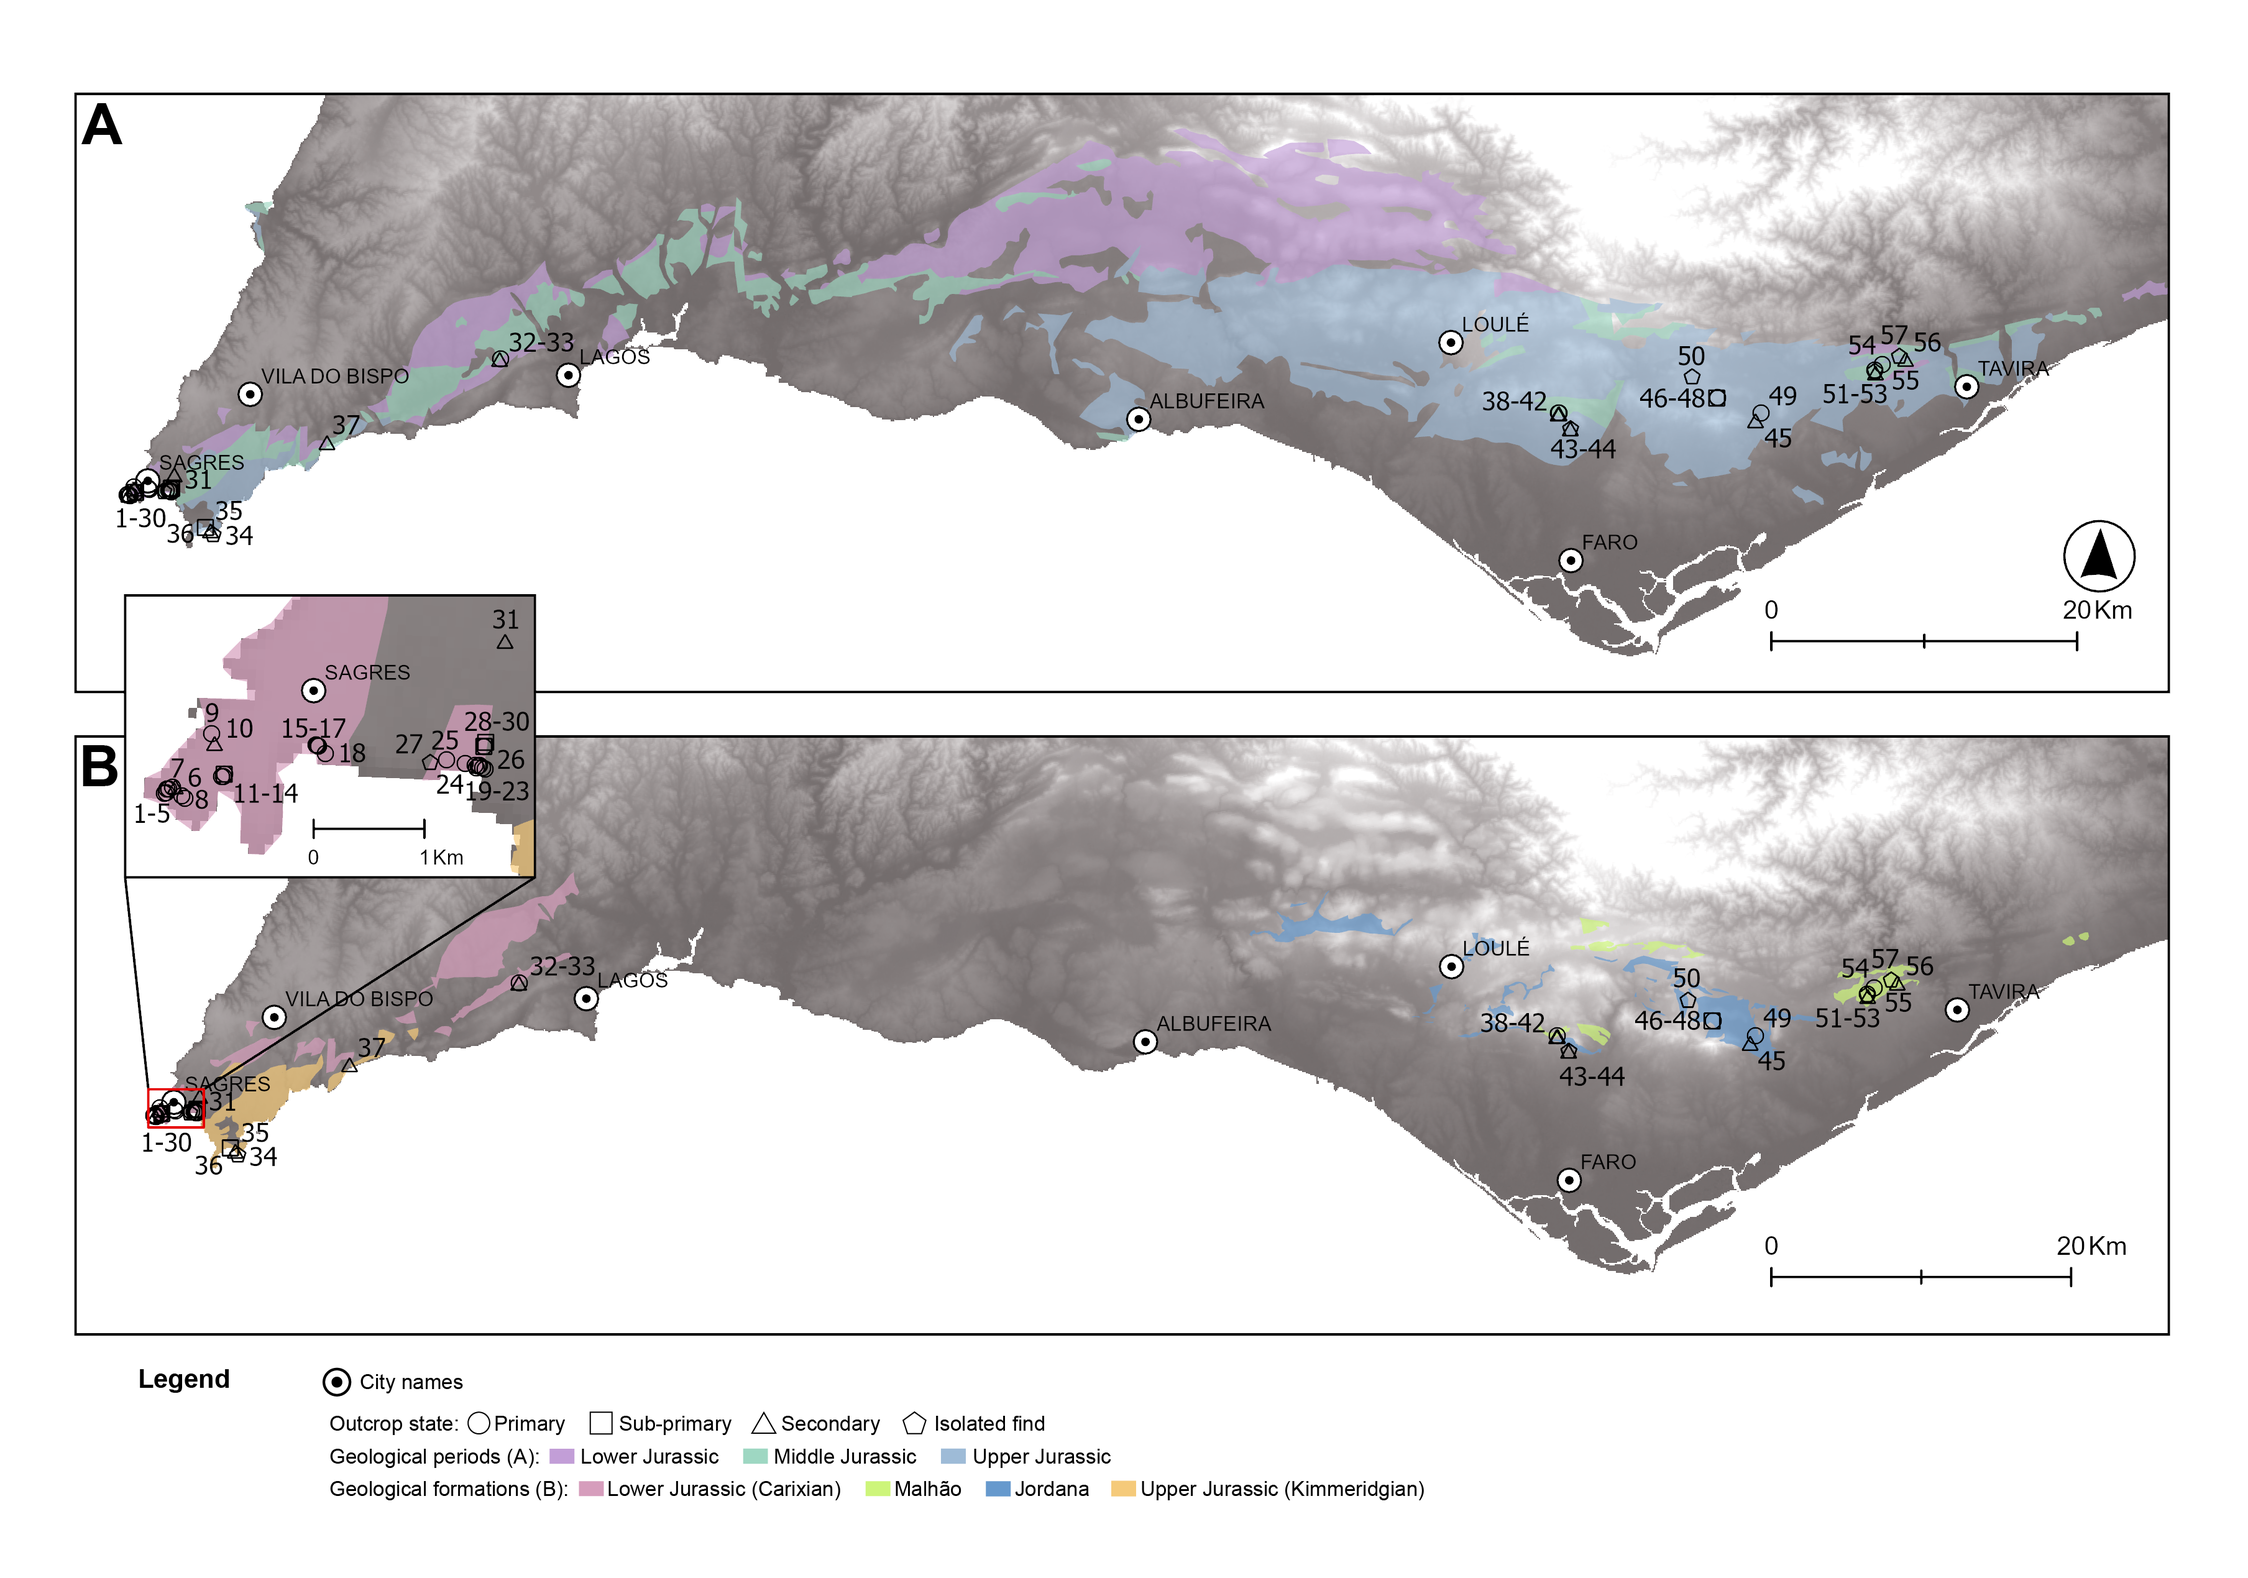
\includegraphics{figures/creating-frames/sources_map.png}

}

\caption{\label{fig-frames-sourcesmap}Map of southern Portugal
(Algarve), with geological samples recovered during this study's
fieldwork. Colors represent the chert-bearing formations in the Algarve.
Numbers represent the recovered samples during fieldwork organized by
formation, outcrop, and location. Lower Jurassic (Carixian) formation:
1-8: Cabo de S. Vicente(CSV); 9-10: Aspa (ASP); 11-14: Foz dos fornos
(FZF); 15-18: Ponta dos Altos (PdA); 19-27: Praia de Belixe (PBX);
28-30: Belixe Sul (BLS); 32-33: Ferrel (FER). Upper Jurassic
(Kimmeridgian) formation: 35: Ponta da Atalaia (PtA); 36: Praia da
Mareta (MAR); 37: Praia da Andorinha (AND). Malhão formation: 38-42:
Casal da colina (CdC); 43: Guilhim (GUI); 45: Caliços (CAL); 51-53:
Oliveiras (OLV); 54-55: Malhão (MALH). Jordana formation: 46-49: Jordana
(JOR); 50: Peral (PER). Isolated finds: 31: Belixe Norte (BLN); 34:
Ponta da Atalaia (PtA); 44: Guilhim (GUI); 56: Descampado (DESCAM); 57:
Pedreira (PEDR). The geological layers were obtained through
vectorization of the geological raster maps (Carta Geológica de
Portugal, 1:500 000 scale) made available by LNEG (Laboratório Nacional
de Energia e Geologia) in https://geoportal.lneg.pt/mapa/. The base maps
were created from a 30×30‐m pixel Digital Elevation Model (DEM) obtained
from the Shuttle Radar Topography Mission
(https://www2.jpl.nasa.gov/srtm/dataprod.htm).}

\end{figure}%

\begin{longtable}[]{@{}
  >{\raggedright\arraybackslash}p{(\columnwidth - 14\tabcolsep) * \real{0.0960}}
  >{\raggedright\arraybackslash}p{(\columnwidth - 14\tabcolsep) * \real{0.1680}}
  >{\raggedright\arraybackslash}p{(\columnwidth - 14\tabcolsep) * \real{0.1120}}
  >{\raggedright\arraybackslash}p{(\columnwidth - 14\tabcolsep) * \real{0.1280}}
  >{\raggedright\arraybackslash}p{(\columnwidth - 14\tabcolsep) * \real{0.1360}}
  >{\raggedright\arraybackslash}p{(\columnwidth - 14\tabcolsep) * \real{0.1280}}
  >{\raggedright\arraybackslash}p{(\columnwidth - 14\tabcolsep) * \real{0.1440}}
  >{\raggedright\arraybackslash}p{(\columnwidth - 14\tabcolsep) * \real{0.0880}}@{}}

\caption{\label{tbl-frames-outcropdata}Outcrop and nodule information
for all recovered samples. The age was defined based on the location of
the outcrops, taking into consideration previous research work and
geological maps. Samples which were isolated or in untrackable secondary
deposition settings do not have a defined geological age.}

\tabularnewline

\toprule\noalign{}
\begin{minipage}[b]{\linewidth}\raggedright
Sample ID
\end{minipage} & \begin{minipage}[b]{\linewidth}\raggedright
Outcrop name
\end{minipage} & \begin{minipage}[b]{\linewidth}\raggedright
State
\end{minipage} & \begin{minipage}[b]{\linewidth}\raggedright
Age
\end{minipage} & \begin{minipage}[b]{\linewidth}\raggedright
Chert morphology
\end{minipage} & \begin{minipage}[b]{\linewidth}\raggedright
Chert frequence
\end{minipage} & \begin{minipage}[b]{\linewidth}\raggedright
Chert variability
\end{minipage} & \begin{minipage}[b]{\linewidth}\raggedright
Chert size
\end{minipage} \\
\midrule\noalign{}
\endhead
\bottomrule\noalign{}
\endlastfoot
SP3\_CSV & Cabo S. Vicente & Primary & Lower Jurassic & Nodule/Bedded &
Sporadic & Homogeneous & 2-5cm \\
SP4\_CSV & Cabo S. Vicente & Primary & Lower Jurassic & Bedded &
Abundant & Homogeneous & - \\
SP6\_CSV & Cabo S. Vicente & Primary & Lower Jurassic & Bedded &
Abundant & Variable & - \\
SP7\_CSV & Cabo S. Vicente & Primary & Lower Jurassic & Nodule/Bedded &
Abundant & Homogeneous & - \\
SP8\_PdA & Ponta dos Altos Este & Primary & Lower Jurassic & Nodule &
Sporadic & Variable & 5-20cm \\
SP9\_PdA & Ponta dos Altos Este & Primary & Lower Jurassic & Nodule &
Abundant & Variable & 5-20cm \\
SP10\_PdA & Ponta dos Altos Este & Primary & Lower Jurassic & Nodule &
Abundant & Homogeneous & 5-10cm \\
SP12\_PBX & Praia do Belixe & Primary & Lower Jurassic & Nodule &
Sporadic & Homogeneous & - \\
SP13\_PBX & Praia do Belixe & Primary & Lower Jurassic & Nodule &
Abundant & Variable & Max. 15cm \\
SP14\_PBX & Praia do Belixe & Primary & Lower Jurassic & Nodule/Bedded &
Abundant & Variable & Max. 15cm \\
SP15\_PBX & Praia do Belixe & Primary & Lower Jurassic & Nodule/Bedded &
Abundant & Homogeneous & Max. 20cm \\
SP16\_PBX & Praia do Belixe & Primary & Lower Jurassic & Nodule &
Abundant & Homogeneous & 3cm \\
SP17\_PBX & Praia do Belixe & Primary & Lower Jurassic & Nodule &
Abundant & Variable & 5-15 cm \\
SP18\_PBX & Praia do Belixe & Primary & Lower Jurassic & Nodule/Bedded &
Abundant & Variable & - \\
SP19\_PBX & Praia do Belixe & Primary & Lower Jurassic & Nodule & Rare &
Variable & 5-20cm \\
SP20\_BLS & Belixe Sul & Sub-primary & Lower Jurassic & Block & Abundant
& Variable & - \\
SP21\_BLS & Belixe Sul & Sub-primary & Lower Jurassic & Nodule &
Abundant & Variable & 3-8cm \\
SP22\_BLS & Belixe Sul & Primary & Lower Jurassic & Nodule & Sporadic &
Homogeneous & 3-8cm \\
SP23\_BLN & Belixe Norte & Secondary & N/A & - & Abundant & Variable &
- \\
SP24\_CSV & Cabo S. Vicente & Primary & Lower Jurassic & Nodule &
Sporadic & Homogeneous & 5cm \\
SP25\_CSV & Cabo S. Vicente & Primary & Lower Jurassic & Nodule & Rare &
Homogeneous & - \\
SP26\_CSV & Cabo S. Vicente & Secondary & Lower Jurassic & - & Abundant
& Homogeneous & - \\
SP27\_CSV & Cabo S. Vicente & Primary & Lower Jurassic & Nodule & Rare &
Homogeneous & 5-10cm \\
SP28\_ASP & Aspa & Primary & Lower Jurassic & Nodule & Sporadic &
Variable & 5cm \\
SP29\_ASP & Aspa & Secondary & Lower Jurassic & - & Abundant & Variable
& \textless5cm \\
SP30\_FZF & Foz dos Fornos & Primary & Lower Jurassic & Nodule & Rare &
Homogeneous & Max. 15cm \\
SP31\_FZF & Foz dos Fornos & Sub-primary & Lower Jurassic & Nodule &
Abundant & Variable & \textless5cm \\
SP32\_FZF & Foz dos Fornos & Primary & Lower Jurassic & Nodule &
Abundant & Variable & 4-8cm \\
SP33\_FZF & Foz dos Fornos & Primary & Lower Jurassic & Nodule &
Abundant & Variable & 4-8cm \\
SP34\_PdA & Ponta dos Altos Este & Primary & Lower Jurassic & Nodule &
Abundant & Variable & 4-8cm \\
SP35\_BLX & Belixe & Isolated find & N/A & - & - & - & - \\
SP36\_PtA & Ponta da Atalaia & Isolated find & N/A & - & - & - & - \\
SP37\_PtA & Ponta da Atalaia & Secondary & Upper Jurassic & - & Abundant
& Variable & - \\
SP39\_AND & Andorinha & Secondary & Upper Jurassic & - & Sporadic &
Homogeneous & - \\
SP40\_FER & Ferrel & Primary & Lower Jurassic & Nodule & Abundant &
Variable & - \\
SP41\_FER & Ferrel & Secondary & Lower Jurassic & - & Sporadic &
Variable & - \\
SP47\_CdC & Casal da Colina & Primary & Middle Jurassic & Nodule & Rare
& Homogeneous & 3-8cm \\
SP48\_CdC & Casal da Colina & Secondary & Middle Jurassic & - & Rare &
Variable & - \\
SP49\_CdC & Casal da Colina & Secondary & Middle Jurassic & - & Rare &
Variable & - \\
SP50\_CdC & Casal da Colina & Primary & Middle Jurassic & Nodule &
Sporadic & Homogeneous & 3-5cm \\
SP52\_CdC & Casal da Colina & Secondary & Middle Jurassic & - & Rare &
Homogeneous & - \\
SP53\_GUI & Guilhim & Secondary & Middle Jurassic & - & Sporadic &
Variable & - \\
SP54\_GUI & Guilhim & Isolated find & N/A & - & - & - & - \\
SP55\_CAL & Caliços & Secondary & Middle Jurassic & - & Rare &
Homogeneous & - \\
SP56\_JOR & Jordana & Sub-primary & Upper Jurassic & Nodule & Abundant &
Homogeneous & 2-20cm \\
SP57\_JOR & Jordana & Primary & Upper Jurassic & Nodule & Abundant &
Homogeneous & 2-5cm \\
SP58\_JOR & Jordana & Primary & Upper Jurassic & Nodule & Sporadic &
Homogeneous & 5cm \\
SP59\_JOR & Jordana & Primary & Upper Jurassic & Nodule & Abundant &
Homogeneous & 3-5cm \\
SP61\_PER & Peral & Other & Upper Jurassic & Nodule & Sporadic &
Homogeneous & 2-5cm \\
SP62\_OLV & Oliveiras & Secondary & Middle Jurassic & - & Abundant &
Variable & - \\
SP63\_OLV & Oliveiras & Primary & Middle Jurassic & Nodule & Sporadic &
Homogeneous & 2-15cm \\
SP64\_OLV & Oliveiras & Isolated find & N/A & - & - & - & - \\
SP65\_MALH & Malhão & Primary & Middle Jurassic & Nodule & Sporadic &
Homogeneous & 5cm \\
SP66\_MALH & Malhão & Primary & Middle Jurassic & Nodule & Sporadic &
Homogeneous & 5cm \\
SP67\_DESCAM & Cabeço Descampado & Secondary & N/A & Nodule & Sporadic &
Homogeneous & - \\
SP68\_PEDR & Pedreira & Other & N/A & - & Rare & Homogeneous & - \\
SP69\_MAR & Praia da Mareta & Sub-primary & Upper Jurassic & Nodule &
Abundant & Variable & Max. 25cm \\

\end{longtable}

\subsection{Western Algarve}\label{western-algarve}

On the westernmost areas of the Algarve, there are mainly cherts from
two different formations: Carixian formations (Lower Jurassic) and
Kimmeridgian formations (Upper Jurassic,
Figure~\ref{fig-frames-sourcesmap}). The latter can be found in primary
deposition in a single known outcrop - Praia da Mareta (MAR) -- or
nearby, in secondary deposition settings. Lower Jurassic outcrops are
more common and, for that reason, have been more studied (Ribeiro 2005).
These outcrops are heterogeneous, showing different geological
characteristics and chert colors (@fig-frames-ljmacro). The Lower
Jurassic cherts can be grouped into three main macroscopic types based
on color (individual Munsell Color Chart codes can be found in the
macroscopic description analysis table) and presence of fossil content:
1) multicolored, yellow, red, light gray or purple type (MC,
Figure~\ref{fig-frames-ljmacro} b and Figure~\ref{fig-frames-ljmacro}
d); 2) single grey/brown type (SGB, Figure~\ref{fig-frames-ljmacro} e
and Figure~\ref{fig-frames-ljmacro} f); 3) multicolored, yellow, red,
light gray or purple with fossils type (MCF,
Figure~\ref{fig-frames-ljmacro} a and Figure~\ref{fig-frames-ljmacro}
c). The first two types are present in all outcrops. They are mainly
characterized by dull to medium luster and opaque translucency, although
some samples were sub-translucent. The feel ranges between smooth and
semi-smooth, although many of the cherts from the Belixe outcrop are
distinctly rough to the touch. In the MC cherts, fossil content is
present but visible only as white, red, or yellow speckling. The SGB
cherts show little fossil content, barely visible with the
stereomicroscope. The MCF show a large quantity of larger fossils
(\textasciitilde1000 µm), which are easily seen by the naked eye and can
be identified under the microscope.

\begin{figure}

\centering{

\includegraphics{figures/creating-frames/macro_lowerJ_west.png}

}

\caption{\label{fig-frames-ljmacro}View of the macroscopic variability
of the Lower Jurassic Carixian cherts (several outcrops) from western
Algarve. (a) Sample SP34\_PdA. (b) Sample SP14\_PBX. (c) Sample
SP16\_PBX. (d) Sample SP30\_FZF. (e) SP9\_PdA. (f) Sample SP34\_PdA.}

\end{figure}%

Petrographically, the Lower Jurassic cherts of western Algarve are
composed mainly of microcrystalline quartz, with textures that range
mostly from wackestone to packstone (@fig-frames-ljwest). Dolomite is
also present although in frequencies inferior to 10\%. Macrocrystalline
quartz and chalcedony occur in small frequencies (\textasciitilde5\%),
frequently replacing bioclasts. The presence of mica is uncommon and
always below 1\%. Allochems present are mostly iron oxides (ranging from
uncommon to very frequent) and the presence of peloids is rare. In more
than 50\% of the samples, no fossils can be identified, as all fossils,
albeit common to very frequent, are poorly preserved, and without any
identifiable morphology. Whenever identifiable, fossils present in the
sample are Echinoderms (@fig-frames-ljwest b and @fig-frames-ljwest c),
Radiolarians, Sponge spicules, and bivalve shells (@fig-frames-ljwest e
and Figure~\ref{fig-frames-ljwest} f). In all samples porosity ranges
from 1-5\% (vuggy type).

\begin{figure}

\centering{

\includegraphics{figures/creating-frames/lowerJ_west.png}

}

\caption{\label{fig-frames-ljwest}Macroscopic and microscopic view of
chert samples from the Lower Jurassic cherts from western Algarve. (a)
Sample SP7\_CSV. Macroscopic view with a stereomicroscope. (b-c) Sample
SP7\_CSV. Microscopic view of thin section, XPL (b) and PPL (c). An
Echinoid spine, replaced by quartz but preserving the fossil's original
structure is present in the center of the images. (d) Sample SP34\_PdA.
Macroscopic view with a stereomicroscope. (e-f) Sample SP34\_PdA.
Microscopic view of thin section, XPL I and PPL (f). Detail of a bivalve
shell replaced by at least two generations of quartz: microcrystalline
quartz at the edges and macrocrystalline quartz inside of the shell.}

\end{figure}%

Despite the similar characteristics between these cherts, the outcrops
are heterogeneous and show varying characteristics between them, which
may be of importance to distinguish between chert sources within the
Lower Jurassic formation. These outcrops have been divided into four
groups, following the available literature: 1) Cabo de S. Vicente (CSV)
and Aspa (ASP); 2) Foz dos Fornos (FZF) and Ponta dos Altos (PdA); 3)
Praia do Belixe (PBX, which includes Belixe Sul, BLS), and 4) Ferrel
(FER). The Cabo de S. Vicente (CSV) and Aspa (ASP) chert outcrops are
characterized by abundant nodules in the natural rock banks of the
cliffs, appearing as horizontal layers within the parent rock. The banks
seem to be mainly dolomite or dolomitic limestones. The process of
dolomitization seems to have affected the chert nodules, as they often
present different levels of silicification from the peripheral areas of
the nodule to the interior, which also affects the size and feel of the
grain. In this case, the peripheral areas of the chert nodules are more
dolomitized, with visible grain and distinctively rough to the touch,
while the interior areas are more silicified and conversely finer and
smoother. The nodules vary in size, ranging from small 4 cm in diameter
circular nodules to bed-like groups of nodules with \textasciitilde20 cm
in width. At the Aspa outcrops, the nodules are less frequent and
smaller. Due to the proximity to the cliffs, the visibility of the chert
nodules is good, and in present times, small chunks of chert (without
cortex or with small amounts of parent rock attached) accumulate in
secondary deposits nearby. Foz dos Fornos (FZF) and Ponta dos Altos
(PdA) show similarities to the CSV outcrops. The nodules are visible in
several banks of dolomite, dolomitic limestone, and limestone, partially
covered by soil and sand. The nodules can be circular, around 5 cm in
diameter, or wide nearly 20 cm in width. Despite their size, these
cherts are frequently filled with fractures that fragment the larger
nodules into smaller volumes of raw material. Alike CSV, FZF and PdA
also show cherts with differing degrees of dolomitization, although in
apparent smaller quantities than CSV. Besides the abundant presence of
primary outcrops, there are also abundant chert nodule fragments in
secondary deposition, down the slope of the cliff (in the case of FZF)
or at the top of the cliff, on a sand path (in the case of PdA). These
are small, between 1-4 cm in width, but of easy access. Between the FZF
chert and the PdA, the main differences seem to be the cortex and parent
rock, which show differing reactions to hydrochloric acid, the first
being dolomite or dolomitic limestone, and the second being mostly
limestone, with some degree of dolomitization in certain areas. Praia do
Belixe (PBX) is characterized by the abundance of chert nodules
throughout the dolomite layers of the cliff area. They are visible in
certain areas of the cliff and within the rock shelters. The nodules can
be small, around 5 cm in diameter, sometimes reaching more than
\textasciitilde30 cm in width, or bedded, as chert layers between the
dolomite layers. The cherts show varying degrees of dolomitization and
are mostly characterized by a coarse to semi-smooth feel and dull
luster, often showing fractures and alterations. Unlike the other
outcrops, no chert nodule fragments were found close to the cliffs, and
the samples could only be recovered directly from the embedded nodules
in the cliff walls. Nodules scattered on the floor were only located at
Belixe Sul (BLS), a primary outcrop nearly destroyed located on a field,
north of the beach area. The chert in this outcrop showed no differences
from PBX, aside from the size of the nodules, which were smaller and
often showed signs of post-depositional alterations. A third location
for chert has been previously identified north of BLS. Belixe Norte
(BLN) is located on a dirt road and an unused agriculture field. Several
chert fragments were collected in this location. However, BLN is in
proximity to an archaeological site and several collected samples were
lithic artifacts. No larger nodules or outcrop were identified in this
location. The samples recovered from the location also seem to
corroborate that BLN should not be considered an outcrop, as they do not
match the local cherts and rather, resemble most of the samples
recovered from eastern Algarve. Ferrel (FER), unlike the other outcrops,
is located inland and away from the coast. Due to its location in a
homonymous village, the state of the outcrop is poor, and all samples
were either recovered as scattered nodules or from larger blocks of
rock, from a partially destroyed outcrop. The proximity of an
archaeological site nearby also raises questions regarding the nodules
found in secondary deposition, as these may be surface finds. Despite
these caveats, the recovered samples are similar to those from the other
Lower Jurassic outcrops, albeit with better quality, being characterized
by a shiny to medium luster and smooth to semi-smooth feel. All surface
fragments and nodules were small, with around 2 to 3 cm of width which
may be explained by the state of the outcrop.

Contrasting with the diversity and quantity of the Lower Jurassic
outcrops, there is only one identified outcrop for Upper Jurassic cherts
in western Algarve, located at Praia da Mareta (MAR) and abundant, or in
a secondary deposition at Ponta da Atalaia (PtA). The Upper Jurassic
cherts are very similar to the Lower Jurassic, with dull to medium
luster and grey/purple colors (@fig-frames-ujwest a). The translucency
ranges from opaque to areas where the chert is translucent. This
translucency may be a significant difference to distinguish between
outcrops. Petrographically, the cherts are also similar to the Lower
Jurassic ones. The only identifiable difference is the presence of
calcispheres. All samples from the MAR and PtA outcrops seen under the
petrographic microscope showed the presence of abundant calcispheres
(@fig-frames-ujwest b and Figure~\ref{fig-frames-ujwest} c), which is
not always apparent with the stereomicroscope. Based on the presence of
calcispheres, we may also consider the samples recovered at Andorinha
(AND) to be Upper Jurassic (@fig-frames-ujwest e and
Figure~\ref{fig-frames-ujwest} f), which were uncommon and scattered at
the top of the cliffs by the beach.

\begin{figure}

\centering{

\includegraphics{figures/creating-frames/upperJ_west.png}

}

\caption{\label{fig-frames-ujwest}Macroscopic and microscopic view of
chert samples from the Upper Jurassic cherts from western Algarve. (a)
Sample SP36\_PtA. Macroscopic view with a stereomicroscope. (b-c) Sample
SP36\_PtA. Microscopic view of thin section, XPL (b) and PPL (c).
Several unidentifiable fossils can be seen in the photo, along with
calcispheres. (d) Sample SP39\_AND. Macroscopic view with a
stereomicroscope. (e-f) Sample SP39\_AND. Microscopic view of thin
section, XPL I and PPL (f). A small amount of calcispheres is present in
the image, along with few unidentifiable fossils replaced by
quartz/chalcedony.}

\end{figure}%

At Praia da Mareta the nodules are only easily accessible on the beach,
where large boulders falling off the cliff (\textasciitilde1 m in
diameter) are transported by the waves. Several chert nodules of
different sizes can be found in the parent rock washed ashore, ranging
between 2 cm to 20 cm in diameter. The quality of the chert also varies,
possibly related to different dolomitization stages of the nodules,
although this may also be influenced by chemical and physical
alterations to the chert. At Ponta da Atalaia the chert can be found
atop the cliffs, with rare nodules scattered on the floor.

\subsection{Eastern Algarve}\label{eastern-algarve}

On the eastern part of the Algarve, chert-bearing known formations are
from the Middle and Upper Jurassic, known as the Malhão formation and
the Jordana formation, respectively. The Malhão formation chert (Middle
Jurassic) was identified in three outcrops: 1) Casal da Colina (CdC); 2)
Oliveiras (OLV); and 3) Malhão (MALH). Whenever in a primary outcrop,
this chert was homogeneous. Secondary deposits were also
identified---Casal da Colina (CdC), Guilhim (GUI), Caliços (CAL) and
Oliveiras (OLV) and were located in recent waterlines and slope
deposits, and the cherts were often characterized by intense
post-depositional alterations (in these cases, it was not possible to
confirm the outcrop location). In the Malhão formation outcrops, the
nodule frequency varied from common to abundant. The nodules are
roundish, ranging between 3 to 5 cm in maximum width. In all cases,
access to the outcrops was easy. Although the parent rock was hard,
several chert nodules could be collected from the surface, accumulating
further down in gentle slope deposits. The Malhão cherts show two
differing macroscopic characteristics: pink/reddish/light gray cherts
(@fig-frames-mjplate b) and grey cherts (@fig-frames-mjplate a). In
general, they are both characterized by a dull to medium luster, opaque
to sub-translucent translucency, and smooth to semi-smooth feel. They
are easily identifiable through the high amounts of macroscopically
visible inclusions, which look like white speckling in plain sight.
Under the stereomicroscope, several round fossils and long spicule-like
shapes can be identified. The petrographic analysis shows that the
Malhão formation cherts are characterized by a wackestone texture, and
composed of microcrystalline quartz (85-95\%). Dolomite is also present
(10-5\%), as well as chalcedony and macrocrystalline quartz
(\textless5\%) frequently replacing fossils. Identified allochems are
oxide patina, ranging from very frequent to uncommon. A high variety of
identifiable fossils (although all are poorly preserved
(@fig-frames-mjplate) were also identified. These fossils are Sponge
spicules (@fig-frames-mjplate e and Figure~\ref{fig-frames-mjplate} f),
Radiolarians, Ostracods (@fig-frames-mjplate c and
Figure~\ref{fig-frames-mjplate} d), Echinoderms, Calcispheres, and
possibly Tentaculites. Porosity in the samples occurs in small
frequencies (\textless5\%), of vuggy type.

\begin{figure}

\centering{

\includegraphics{figures/creating-frames/middleJ_east.png}

}

\caption{\label{fig-frames-mjplate}Macroscopic and microscopic views of
Middle Jurassic chert samples from the Malhão formation. (a) Sample
SP50\_CdC, macroscopic view with a stereomicroscope. (b) Sample
SP62\_OLV, macroscopic view with a stereomicroscope. (c-d) Microscopic
view of SP50\_CdC, XPL (c) and PPL (d). Detail of a fossil (possibly an
Ostracod), replaced by two generations of chalcedony (1st generation in
the outer edges and 2nd generation replacing the inside). (e-f)
Microscopic view of SP54\_GUI, XPL (e) and PPL (f). General view of the
thin section. Several fossil ghosts can be seen. Despite the poor
preservation, it may be possible to identify a few fossils based on the
size and morphology: 1) calcispheres or recrystallized radiolarians; 2)
monaxon spicules pointed at one end.}

\end{figure}%

The Jordana formation chert (Upper Jurassic) was identified in one area
in the Algarve (@fig-frames-sourcesmap), in an outcrop of the same name
(JOR). Whenever in a primary outcrop, the chert was homogeneous,
although alternated with nodules of other lithologies within the parent
rock. No chert was identified in any secondary deposits, which might be
related to the anthropic alteration of the landscape. Smaller nodules
broken from the parent rock were identified near the primary source in a
field. Whenever embedded in the parent rock, the nodules varied in size
(\textasciitilde1-10 cm) and were abundant, with a high level of
difficulty in their removal, due to the hardness of the parent rock. The
cherts show little macroscopic variability between nodule and outcrop.
They are grey/brown (with visible yellow inclusions)
(@fig-frames-ujplate a and Figure~\ref{fig-frames-ujplate} b). Within
nodules, however, the cherts are heterogeneous, with dull and shiny or
smooth and semi-smooth feel areas. Some of the nodules also show
variability of translucency, with translucent areas, with a very fine
grain, and little presence of visible inclusions. The petrographic
analysis shows that the cherts range from a wackestone to packstone
texture (@fig-frames-ujplate), which was already seen macroscopically.
They are composed mostly of microcrystalline quartz (90-99\%), with the
presence of fibrous chalcedony (1\%) replacing the fossils and dolomite
(1\%), as well as negligible percentages of other minerals. Present
allochems are iron oxides, ranging between very frequent to common.
Albeit frequent, fossils are poorly preserved in general, with a few
being identifiable: Calcispheres (@fig-frames-ujplate c and
Figure~\ref{fig-frames-ujplate} d), Bivalve shell (@fig-frames-ujplate e
and Figure~\ref{fig-frames-ujplate} f), Sponge spicules, Ostracod,
Echinoderms, and Gastropod. Porosity is small (\textasciitilde1\%) of
vuggy type.

\begin{figure}

\centering{

\includegraphics{figures/creating-frames/upperJ_east.png}

}

\caption{\label{fig-frames-ujplate}Macroscopic and microscopic views of
the Upper Jurassic chert samples from the Jordana formation. (a) Sample
SP58\_JOR, macroscopic view with a stereomicroscope. (b) Sample
SP59\_JOR, macroscopic view with a stereomicroscope. (c-d) Microscopic
view of SP56\_JOR, XPL (c) and PPL (d). General view of calcispheres in
an area of the chert characterized by a large concentration of oxide
patina and opaques. (e-f) Microscopic view of SP58\_JOR, XPL (e) and PPL
(f). General view of the thin section. A large bivalve shell fragment is
visible at the top.}

\end{figure}%

\subsection{Other outcrops}\label{other-outcrops}

It is important to note that the aforementioned chert geological samples
represent the chert variability of the identified chert-bearing
formations and outcrops. However, a small number of outcrops described
in regional geological maps were not identified or were not accessible.
This includes four outcrops: 1) a Lower Jurassic outcrop with chert
micronodules which was identified through a geological profile (Oliveira
1992); 2) a Middle Jurassic outcrop located at the easternmost section
of the Algarve with partially dolomitized clasts and chert nodules
(Oliveira 1992); 3) several unprospected locations from previous
geoarchaeological works, all related to the Peral Anticline and reaching
from central to eastern Algarve; 4) a possible chert exploitation
archaeological site located on top of a chert source (Monte do Cerro),
in eastern Algarve which was not identified and is possibly inaccessible
(Nuno Bicho et al. 2003). All of these unidentifiable outcrops are
located in the central or eastern portion of the Algarve. This may be
related to the frequent landscape changes occurring due to agriculture
or the population of previously uninhabited areas, which seldom occurs
in western Algarve by the cliff areas, where most outcrops are located.

\section{Discussion}\label{discussion}

The survey work and analyses of the collected geological samples show
that the south of Portugal has a high potential for chert raw material
studies. The presence of chert-bearing geological formations throughout
the Algarve would provide several possibilities for sourcing and
procurement whenever groups moved throughout the territory. This is
further important when we consider the geology of this region. The
geology of the Algarve itself may have played an important part in how
groups procured their raw materials, specifically, their chert, a task
that has been identified as essential for hunter-gatherer groups. To the
south, communities would only have access to chert-bearing outcrops down
to the coast. To the north, the mountain range would not only have
provided no chert nodules but may have also hampered the movement of
populations, forcing groups to move east and west instead of north or
south. This movement may have facilitated the gathering of cherts from
different formations within the Algarve, posteriorly then brought into
the sites. Especially for Middle and Upper Paleolithic occupations,
understanding the sources of chert in the Algarve may provide data about
where in the territory these groups were sourcing their chert raw
materials, and how they were using the territory having in consideration
the region's natural barriers and consequent distribution of resources.
Although this topic remains unexplored, this study stands as a further
step to tackle these questions in the Algarve, as it may provide the
necessary basis for comparative studies with archaeological assemblages.
However, tracking these movements and procurement patterns is only
possible if the cherts from the different formations and outcrops can be
traced back to their sources. This presented itself as the first caveat
for this type of study, since for the Algarve, for example, all cherts
formed in Jurassic formations in pelagic environments. Despite the
similar formation environments, in general, there seem to be relevant
differences between the cherts of different formations and periods. This
is further relevant given the fact that they are geographically distant.
Within formations, however, there are no discernable differences, both
at a macroscopic and petrographic level, as these do not seem to be
useful to distinguish between outcrops. This is most obvious on the
Lower Jurassic formation of western Algarve. The identified chert
groups, which varied mostly in color and fossil content, are present in
several outcrops from this formation. In this region, the variables
which may be better used to understand which outcrops were visited may
be the quality (differing levels of dolomitization, presence/absence of
fractures or even size of grain) and size of the nodules. The latter,
for example, is an important variable in the Praia do Belixe outcrops,
which show the largest volumes of rock, even if the chert's quality is
worse than some other available, smaller nodules. Size may be used in
conjunction with other technological data, to understand whether
different nodules were being explored differently based on their size,
or their procurement was being preferred in relation to other smaller
nodules in possibly closer outcrops in the region. The Upper Jurassic
nodules of western Algarve also show larger volumes than those from the
Lower Jurassic. Translucency also seems to be a good macroscopic
indicator to distinguish between western Algarve Lower and Upper
Jurassic cherts, since the latter are characterized as sub-translucent.
However, for a reliable distinction between the Lower Jurassic and the
Upper Jurassic cherts, petrographic analyses and the identification of
calcispheres may be necessary. The differences identified among the
cherts of the various formations can be seen both at a macroscopic and
petrographic level. Given the formation settings, petrographically, all
the cherts from the Algarve are fairly homogeneous - marine origin, in
limestone or dolomitic limestone rocks, all formed during the Jurassic.
The use of specific fossils for the identification of the cherts is also
difficult since these are often not well preserved enough to allow the
identification of species that may connect a group of cherts. The size,
frequency, and preservation state of the fossils seem to be, then, one
of the defining criteria for discerning cherts from different
formations, and thus, different geographic areas. These characteristics
seem to be observable macroscopically, as well, allowing the cherts from
the three different areas and formations -- West (including the Lower
Jurassic and Upper Jurassic formation cherts of western Algarve),
Jordana, and Malhão - to be differentiated without the need for thin
sections (@fig-frames-macrocomparison). An exception might be the
distinction between the cherts from the West and Malhão - the reddish
cherts from Malhão are visually indistinguishable from those from the
West with a higher fossil content. The grey cherts of the Malhão Middle
Jurassic formation do show a higher concentration of visible round
fossils, however the distinction is only possible seen under the
stereomicroscope and on a fresh surface, which might hamper the
classification of archaeological materials. These distinctions are
especially important for archaeological collections, especially those
which may be small, with small artifacts, or for the study of older
collections to which other (destructive) means of analysis may not be
applied.

\begin{figure}

\centering{

\includegraphics{figures/creating-frames/macro_comparison.png}

}

\caption{\label{fig-frames-macrocomparison}Comparison between the cherts
of different formations in the Algarve, organized by geological age and
formation. (a-b) Lower Jurassic (Carixian formation) chert samples under
the stereomicroscope. (c-d) Middle Jurassic (Malhão formation) chert
samples under the stereomicroscope. (e-f) Upper Jurassic (Jordana
formation) chert samples under the stereomicroscope.}

\end{figure}%

These data seem to confirm the potential of a macroscopic analysis to
study the cherts of the Algarve. Albeit applying different
methodologies, such as petrographic analyses, to these cherts is a way
of completing the petrographic study of a collection, reliably applying
mostly a macroscopic analysis to the assemblages coming from southern
Portugal helps tackle issues such as the destructiveness, costliness,
and time consumption of some methods. Our study was able to provide a
more detailed reference collection for chert outcrops in the Algarve,
which will allow to test models about raw material procurement and use
in a multilayered archaeological site like Vale Boi.

There are, however, some noteworthy caveats in this type of study.
Landscapes have changed through time, both naturally and with the
influence of modern society. House constructions, agricultural fields,
and roads, for example, have modified the landscape, possibly altering
the availability and visibility of raw materials. Other natural
processes, such as the development of biomantle or soil cover may also
hamper raw material visibility in the landscape. Similarly,
environmental changes may have had an impact on raw material
availability, through its impact on surface processes which expose,
erode and transport the raw materials (Pereira and Benedetti 2013). As
such, it is important to keep in mind that current raw material sources,
and specifically chert ones which may be subtly visible in the
landscape, may not correspond to the sources which were available in the
past. Another caveat regarding chert sources, especially in a geographic
area like the Algarve, is the possibility of some outcrops being
submerged. Previous studies have identified the existence of Jurassic
lithologies on the west coast, submerged by water (Terrinha et al.
2006). These were mainly surveys done by oil companies which were able
to obtain the submerged stratigraphies on the southwestern coast of
Portugal and that revealed Jurassic limestones and dolomites, although
the presence of chert is not described and remains unknown. Whether
these submerged lithologies are different from the currently emerged
ones is also uncertain. These studies also revealed that Jurassic
lithologies were covered by more recent geological layers, including
Pliocene and Pleistocene layers, thus forming before and/or during
Paleolithic occupations of the territory (Terrinha et al. 2006). In
times when the sea level was similar to the current one, the submerged
lithologies would not have been accessible, even during low tide.
However, during periods when the sea level was lower due to water
freezing in the polar caps, as during the LGM for example, large
portions of the coast that had been submersed would have been
accessible. During this period, in Portugal, the coast would probably be
close to the continental platform, \textasciitilde120 m below the sea
level (J. Dias, Rodrigues, and Magalhães 1997; J. M. A. Dias et al.
2000). Especifically in western Algarve, the coastline may have been
displaced \textasciitilde10-15 km offshore from the present coastline
(N. Bicho and Haws 2008). Although currently unknown, it may be possible
that during periods like the LGM, limestone and dolomite Jurassic
lithologies, with chert nodules, might have been exposed and available.
When studying chronologies characterized by cold and harsh climatic
conditions with impacts on sea level changes and mixed with coastal
uplift events, it is relevant to keep in mind that the chert variability
present in the current coastline may not necessarily reflect the
variability in the past. Despite these caveats, our data raises the
possibility to understand whether this new portion of landmass altered
the raw material procurement patterns of these groups, or added new
resources which had been previously unavailable. Studies that compare
Gravettian and Magdalenian assemblages (with higher mean sea-levels, and
possibly even similar to current coastlines) to Proto-Solutrean and
Solutrean assemblages (with LGM low mean sea-levels), within one single
site, may give new insights into this question.

\section{Conclusion}\label{conclusion}

In this study we identified several sources of chert nodules in southern
Portugal and characterized the regional cherts, which were of critical
importance for hunter-gatherer communities during the Late Pleistocene.
For this we applied a two-step raw material analysis approach, composed
of macroscopic and petrographic analyses. The results show the presence
of four different chert formations, dispersed in western and eastern
Algarve. Within most formations, there is variability in the nodules and
the outcrops. There are however identifiable macroscopic and
petrographic differences between formations which allow their
distinction. Although the petrographic analysis is essential to identify
the fossils present in the chert, a macroscopic approach seems to be
pertinent for a quick and inexpensive analysis to distinguish between
cherts of the different formations. The presence of chert sources in the
Algarve region, with distinguishable characteristics between formations,
which may be analysed preliminarily through macroscopic approaches,
shows the potential for chert raw material studies of archaeological
sites in this key area. Further steps in our study will include the use
of the data gathered in the present study and the completed LusoLit
lithotheque to study chert use from multi-component sites with Upper
Paleolithic chronologies such as Vale Boi, and participate in the
discussion of human adaptations throughout the Late Pleistocene.
Furthermore, future approaches include the use of geochemical methods to
further characterize these cherts and the integration of the resulting
data in the online database.

\section*{Supporting information}\label{supporting-information}
\addcontentsline{toc}{section}{Supporting information}

\markright{Supporting information}

S1 Table. Field sample/outcrop dataset. Table with recorded data on the
outcrops and cherts, during fieldwork and prospections during 2021 and
2022. S2 Table. Macroscopic analysis dataset. Table with the data
collected from the macroscopic analyses of all chert samples collected
from the fieldwork and prospections during 2021 and 2022. S3 Table. Data
dictionaries for macroscopic and petrographic analyses. Description of
the used variables (including allowed variables and references) for the
macroscopic and petrographic analyses used in the present study.

\section*{Acknowledgments}\label{acknowledgments-1}
\addcontentsline{toc}{section}{Acknowledgments}

\markright{Acknowledgments}

We would like the thank the entities that funded the current research:
Fundação para a Ciência e a Technologia (FCT) and ICArEHB
(Interdisciplinary Center for Archaeology and the Evolution of Human
Behavior). Furthermore, we want to thank Dr.~Telmo Pereira and
Dr.~Carlos Ribeiro for allowing us to consult their previous research
and for their support. We'd like to thank Jack Acres for the IT support
essential for the creation of the online LusoLit database. Finally, we
thank Dr.~Célia Gonçalves for helping with the creation of the maps.

\section*{Author contributions}\label{author-contributions}
\addcontentsline{toc}{section}{Author contributions}

\markright{Author contributions}

\textbf{Conceptualization}: Joana Belmiro, Xavier Terradas, João
Cascalheira. \textbf{Funding acquisition}: Joana Belmiro, João
Cascalheira. \textbf{Investigation}: Joana Belmiro.
\textbf{Methodology}: Joana Belmiro, Xavier Terradas, João Cascalheira.
\textbf{Writing -- original draft}: Joana Belmiro. \textbf{Writing --
review \& editing}: Xavier Terradas, João Cascalheira.

\bookmarksetup{startatroot}

\chapter{Within and beyond: chert procurement patterns during the Upper
Palaeolithic in Southwesternmost
Iberia}\label{within-and-beyond-chert-procurement-patterns-during-the-upper-palaeolithic-in-southwesternmost-iberia}

\textbf{Authors}: Joana Belmiro, Xavier Terradas, Salvador
Dominguez-Bella, João Cascalheira

\newpage

\section*{Abstract}\label{abstract-2}
\addcontentsline{toc}{section}{Abstract}

\markright{Abstract}

Analyses of raw materials and the distinction between local/regional and
long-distance sources have proven invaluable for understanding the
extensive movements, interactions, and social networks during the Upper
Palaeolithic in the Iberian Peninsula. However, unlike other parts of
Iberia, research on the management and acquisition of raw materials in
the south and west of Iberia remains relatively underdeveloped. Despite
significant knowledge about the technological practices of Palaeolithic
hunter-gatherers from southern Portugal, particularly from studies
conducted at the site of Vale Boi, there is a noticeable lack of focus
on raw materials management. This paper presents the first comprehensive
characterization of chert raw materials from the Gravettian,
Proto-Solutrean, and Solutrean occupations at Vale Boi, using both
macroscopic and petrographic techniques. Our study reveals that the
majority of chert found at Vale Boi originates locally, within a 20 km
radius. However, a non-negligible portion of the chert comes from
non-local sources, indicating \textgreater200 km raw material
circulation from central Portugal and southern Spain.

\textbf{keywords:} Upper Paleolithic; Iberian Peninsula; Lithic raw
materials; Petrography

\newpage

\section{Introduction}\label{introduction-2}

Knappable raw materials play a crucial role in understanding the
mobility and lifeways of past hunter-gatherers, given the ubiquitous
presence of lithic artefacts throughout Prehistory. More than mere rocks
with which stone tools were produced, the management of these resources
is intimately connected to a group's technological, social, and cultural
organisation, potentially influencing the group's overall survivability
(Oestmo 2017; Binford 1979; Bleed 1986; Bousman 1993; R. Torrence 1983;
Gould and Saggers 1985).

Several key topics in the study of hunter-gatherer behaviour and
organisation have been explored in different geographic regions and
chronological periods through raw material analysis, such as modalities
of procurement and mobility strategies (Ambrose and Lorenz 1990; Binford
1979; Binford and Stone 1985; Gould 1985; Gould and Saggers 1985; Kuhn
1991; McCall 2007), occupation types and their duration (Kuhn 2004;
Surovell 2009), the establishment and dimension of social networks
(Whallon 2006), as well as exchanges between groups or individuals
(Gamble 1999). These analyses are often achieved by systematically
characterizing geological and archaeological raw materials and
establishing correlations between samples from both origins. The
ultimate aim is to identify the corresponding sources, enabling, for
example, a precise differentiation between local and non-local raw
materials, and examine their distribution within a site over different
occupations and periods.

These approaches and concepts have also been extensively and
successfully applied to the study of lithic assemblages from prehistoric
archaeological sites in the Iberian Peninsula (e.g., Aubry et al. 2016;
Aubry and Igreja 2009; García-Rojas et al. 2021; Gómez de Soler et al.
2020; Herrero-Alonso, Fuertes-Prieto, and Neira-Campos 2020; Matias
2016; Ortega 2003; Pereira, Andrade, et al. 2016; Pereira et al. 2021,
2022; Ramacciotti et al. 2022; Sánchez de la Torre et al. 2023; Soto
2016; Rodríguez, Rodríguez, and Pelegrin 2011; Costa et al. 2022; Nocete
et al. 2005), and contributed to understanding how different groups
explored and managed the available lithic resources.

In this context, raw material analyses and the distinction between
local, regional and long-distance sources have been instrumental in
tracing extensive movements, contacts, and social networks throughout
the Upper Palaeolithic (UP) throughout Iberia. Noteworthy examples
include studies in northwestern Iberia (Galicia) during the Solutrean
period (Hermida, Rellán, and Rodríguez 2016), northern Iberia (Asturias)
during the Magdalenian occupations at Las Caldas (Corchón Rodríguez,
Martínez, and Tarriño 2016), northeastern Iberia (Catalunya) during the
Aurignacian and Gravettian periods at Arbreda cave (Marreiros et al.
2016; Ortega 2003), northern Portugal during the Gravettian/Solutrean
periods in the Côa Valley (Aubry et al. 2016, 2004), and inland central
Iberia (Guadalajara) during the Proto-Solutrean and Solutrean periods at
Peña Capón (Sánchez de la Torre et al. 2023). Ultimately, the
recognition of these connections has broadened our comprehension of
mobility and social organization during the UP in Iberia, illustrating a
vast interconnected territory.

However, in contrast to other areas of Iberia, and despite the potential
of raw material studies to shed light on the lifeways and organisational
structures of Palaeolithic hunter-gatherers, research on the procurement
and management of raw materials during the UP in southern and western
Iberia remains in its initial stages. Specifically, in southern
Portugal, even though there is considerable knowledge about the
technological organisation of Palaeolithic hunter-gatherers---largely
due to research conducted at the Vale Boi archaeological site (see e.g.,
Belmiro et al. 2021; Nuno Bicho et al. 2013; Cascalheira and Bicho 2013;
Marreiros et al. 2015; Cascalheira 2010; Horta, Cascalheira, and Bicho
2019)---raw material studies are notably infrequent and use mainly
macroscopic methodologies.

This situation is attributed to the absence of a detailed and
comprehensive characterization of regional lithic resources in the
Algarve region (southern Portugal) and the subsequent lack of a complete
reference collection produced by complementing characterization
methodologies, which is a critical component for conducting raw material
studies. Such efforts are particularly crucial for distinguishing
between local and non-local raw materials and for understanding
variations within the archaeological record (Pop 2015; Surovell 2009).

Recently, we have made significant strides by introducing such a
reference collection and establishing a framework for raw material
studies in the region, through a detailed macroscopic and petrographic
database of chert resources in the Algarve region (Belmiro, Terradas,
and Cascalheira 2023). This initiative paves the way for systematic
investigations into raw material procurement strategies during the Upper
Palaeolithic, especially concerning the Vale Boi site, where previous
raw material studies have already shown complex patterns of chert
procurement and management. These preliminary studies at Vale Boi,
employing only macroscopic methods, pointed to a predominant use of
local cherts (Nuno Bicho et al. 2013; Pereira, Bicho, et al. 2016;
Verissimo 2004), likely originating within a 16 km radius and reflecting
embedded procurement strategies (Pereira, Bicho, et al. 2016). To a
lesser extent, non-local cherts were also identified throughout the
various UP occupations (Nuno Bicho et al. 2013; Pereira, Bicho, et al.
2016; Verissimo 2004), pointing to extended sourcing networks, possibly
involving sourcing from other regions of southern Portugal and southern
Spain. The presence of chert from the Cretaceous formations of central
Portugal has also been suggested (Nuno Bicho et al. 2013).

These results highlight the potential for systematic raw material
studies at the site to shed light on the lithic resource procurement
strategies, mobility patterns, and social networks of the
hunter-gatherer groups of southwestern Iberia throughout the UP.

Vale Boi stands as a key archaeological site for this study since it is
currently the only site in southern Portugal with a long-term occupation
spanning most of the UP and allowing the exploration of raw material
procurement and mobility trends through time (Cascalheira et al. 2017).
It also holds a pivotal role in the study of UP adaptations on the
Iberian Peninsula, providing invaluable insights into the subsistence
and technological strategies of hunter-gatherer populations (Belmiro et
al. 2021; Nuno Bicho et al. 2013; Cascalheira et al. 2017; Cascalheira
2019; Horta, Cascalheira, and Bicho 2019; Manne et al. 2012; Marreiros
et al. 2016; Pereira, Bicho, et al. 2016).

Furthermore, previous studies have highlighted the role of Vale Boi in
understanding different patterns of territory exploitation and contact
with other regions of Iberia throughout the UP. During the Solutrean,
Vale Boi has been interpreted as an important connection point between
the core Solutrean areas of central Portugal and southern Spain, making
it a key site for identifying extended social networks that promoted the
exchange of information and culture (Cascalheira et al. 2017;
Cascalheira and Bicho 2013; Cascalheira 2013). On the contrary,
techno-typological studies from the Gravettian occupations of Vale Boi
instead show marked differences between regions and suggest a more
limited circulation of people and information in southern Iberia
(Marreiros and Bicho 2013).

Based on the notions that a) during the Solutrean Vale Boi served as a
connection point between different regions which may have promoted the
exchange of information and culture, including raw materials from
long-distances; and b) the limited circulation of people during the
Gravettian may have isolated groups occupying Vale Boi, making them
mostly reliant on the available local or regional resources, we propose
a set of hypotheses and expectations regarding chert procurement and
human mobility throughout the UP at Vale Boi. On one hand, it would be
expected that Solutrean occupations are characterized by the predominant
use of local raw materials but with a considerable percentage of cherts
obtained from long-distance sources, possibly through exchange with
different groups in Iberia. Conversely, it would be expected that
Gravettian occupations would be mostly composed of local cherts, with a
more limited presence of long-distance cherts.

To investigate the applicability of these patterns to the procurement
and circulation of lithic raw materials, and to examine the prevailing
hypotheses concerning UP mobility and social network exchanges, this
paper focuses on the following questions: 1) what types of chert were
the hunter-gatherers of Vale Boi using and where did they come from?; 2)
are there different patterns of chert use throughout time?; 3) and if
so, how can these be related to patterns of land use and the circulation
of people/ideas, as suggested through technological studies of the same
lithic assemblages? As a result, our study presents the first
comprehensive characterisation of chert raw materials, through
macroscopic and microscopic analysis, of UP occupations in southwestern
Iberia, derived from the Gravettian, Proto-Solutrean, and Solutrean
(c.~32-19 ka cal BP) occupations at Vale Boi.

\subsection{Site description}\label{site-description}

Vale Boi is located on the western coast of the Algarve region in
southern Portugal, within a small valley that extends southward to the
Atlantic coast, approximately 2 km away (Figure~\ref{fig-map} b). It is
bordered by limestone outcrops that form rock shelters facing west and
southwest (Nuno Bicho et al. 2007; Nuno Bicho, Cascalheira, and
Marreiros 2012; Nuno Bicho et al. 2013; Cascalheira and Bicho 2013;
Cascalheira et al. 2017; Manne et al. 2012; Manne and Bicho 2011). The
site extends for more than 10,000 sq meters along the slope of the
valley, through which three main areas were excavated between 2000 and
2019: Slope, Terrace, and Shelter. For this study, the chosen areas were
the Terrace and Shelter areas (see Section 2 Materials and Methods).

The Terrace encompasses occupations from the UP to the Early Neolithic,
resulting in the identification of eight main lithostratigraphic units.
The UP sequence includes several occupations attributed to the
Gravettian (levels 8 to 6) between c.~32 and 27 ka cal BP,
Proto-Solutrean (levels 5 to 4E) between c.~26 and 24 ka cal BP, and
Solutrean (level 4D, 4C, 4C, 4 and Lower 3) between c.~24 and 20 ka cal
BP (Belmiro et al. 2021; Cascalheira and Bicho 2013; Cascalheira et al.
2017).

The Shelter area shows four main lithostratigraphic units, with
Magdalenian, Solutrean and Gravettian occupations. From these, the
Solutrean levels show the most intensive occupation, with three,
well-preserved, archaeological horizons (layers C to A) and dated to
c.~24-22 ka cal BP (Cascalheira et al. 2013, 2017; Cascalheira 2010).
These occupation levels were identified under blocks of limestone, which
collapsed from the rockshelter ceiling (Cascalheira 2010).

Both these areas have been previously interpreted as seasonal
residential camps, repeatedly used for extended stays, due to the
abundance of lithic debitage, stone tools, heat-cracked rocks related to
grease rendering activities, large quantities of faunal remains (both
marine and terrestrial) and the presence of ornaments and portable art
(Manne et al. 2012). The analysis of lithic assemblages and retouched
frequency of lithic assemblages from the Terrace and Shelter areas also
corroborate this interpretation (Cascalheira 2010; Marreiros 2009;
Cascalheira et al. 2017). Cascalheira et al. (2017) show that, with the
exception of the Early Gravettian occupations of the Terrace area and
Magdalenian occupation of the Shelter, all other UP occupations are
composed of high-density assemblages with low degree of retouch,
correspondent to a residential base-camp occupation, for extended
periods of time.

\begin{figure}

\centering{

\includegraphics{figures/within-and-beyond/map_layout.png}

}

\caption{\label{fig-map}Iberian Peninsula map with locations and
geological formations mentioned throughout the paper. a) Detail of the
central Portugal region where the Cenomanian formations with chert
nodules are located. b) Detail of southwestern Portugal, with chert and
chalcedony bearing formations, outcrops, and location of Vale Boi. c)
Detail of eastern Algarve with chert-bearing formations. The figure was
produced using ArcGIS Pro 3.2.}

\end{figure}%

\subsection{Regional geological
background}\label{regional-geological-background}

The Algarve region is a complex territory, marked by several geomorphic
sub-regions and geological units that provide different lithological
resources. Two of the main geological units which characterize the
Algarve are: 1) the Baixo Alentejo Flyschoid Group, part of the south
Portuguese Zone (Paulo Fernandes et al. 2012; Oliveira 1984; Onézime et
al. 2003), located in the north sector of the region, and characterized
by schists, greywackes and quartzites; and 2) the Algarve basin in the
south, which is characterized by limestones, dolomites and marls
(Terrinha et al. 2006). It is within these limestones and dolomitized
limestones from the Triassic to the Upper Jurassic where chalcedony and
chert nodules/beds can be found (Manuppella et al. 1987; Manuppella et
al. 2007; Ribeiro 2005; R. Rocha et al. 1979; R. Rocha et al. 1983;
Terrinha et al. 2006).

The availability of regional resources containing cherts and the
characterization of their lithologies has already been published by our
team (Belmiro, Terradas, and Cascalheira 2023), and we herein present
the summarized main findings. The results showed the existence of
abundant chert nodules and beds found in the Lower Jurassic (Carixian)
formation and Upper Jurassic (Kimmeridgian) formation, mostly
outcropping in the cliff and beach areas of westernmost Algarve, at
\textasciitilde20 km southwest from the site of Vale Boi, and with one
single inland outcrop located \textasciitilde8 km east from the site
(Figure~\ref{fig-map} b). The Lower Jurassic nodules and beds can be
found in abundant outcrops, but also frequently in sub-primary or
secondary deposition settings in proximity to the outcrops, possibly due
to natural erosion. However, in the case of the inland outcrop of
Ferrel, the outcrop is partially destroyed due to recent human action,
and chert can be found scattered as chunks or larger nodules. The Upper
Jurassic nodules can be found in sub-primary deposition and are easily
accessible, or in secondary deposition. The cherts from the previously
mentioned formations are are frequently opaque with yellow, grey, purple
or red colours, occasionally with bands or laminations, and frequently
with visible sponge spicules. Although abundant, these chert nodules are
frequently small (\textasciitilde4-10 cm in length), with the largest
nodules being \textasciitilde20 cm, and frequently characterized by high
levels of dolomitization and fractures. Petrographically, they are
composed mainly of microcrystalline quartz, with wackestone or packstone
textures, small percentages of macrocrystalline quartz, fibrous
chalcedony and allochems composed of oxides and poorly preserved
bioclasts. When identifiable, the bioclasts are Echinoderms,
Radiolarians, Sponge spicules and Bivalve shells. The Upper Jurassic
cherts of Mareta show similar petrographic characteristics, but with
abundant Calcispheres which are not always apparent under the
stereomicroscope.

Chert sources were also identified in two formations from the eastern
area of the Algarve (Figure~\ref{fig-map} c). The Middle Jurassic Malhão
formation chert outcrops were identified at around 80-100 km east of the
site and characterized by chert nodules with similar macroscopic
features to those found in western Algarve. Petrographically they are
composed mainly of microcrystalline quartz and characterized by
wackestone textures, while dolomite, chalcedony and macrocrystalline
quartz are also present in small percentages (\textless10\%). Allochems
are iron oxides, and albeit poorly preserved, several bioclasts can be
identified: Sponge spicules, Radiolarians, Ostracods, Echinoderms,
Calcispheres and possibly Tentaculites. The Upper Jurassic Jordana
formation chert outcrops were identified at around 90 km east of Vale
Boi and characterized by chert nodules with significantly different
macroscopic features to those of other formations, with frequently small
sizes (\textasciitilde5 cm), difficult removal from the parent rock and
unidentified secondary deposits. Petrographically they are composed
mostly of microcrystalline quartz, with wackestone to packstone
textures, and small percentages of fibrous chalcedony and dolomite
(\textless10\%). They show frequent iron oxides and very frequent
bioclasts, albeit often poorly preserved and unidentifiable; identified
fossils are Calcispheres, Bivalve shells, Sponge spicules, Ostracods,
Echinoderms and Gastropods.

Chalcedony can be found \textasciitilde10 km west of Vale Boi
(Figure~\ref{fig-map} b), within the marl-carbonated Triassic formations
as lenses or nodules and was formed through hydrothermal processes (Nuno
Bicho et al. 2013). Previous studies also note the presence of
chalcedony (with frequent presence of cortex) in the immediate vicinity
of the site (Pereira, Bicho, et al. 2016; Gibaja Bao and Ferreira Bicho
2013). The chalcedony frequently has fractures and fissures and is
characterized by a fibrous quartz structure, without inclusions or
fossils.

\section{Materials and methods}\label{materials-and-methods-1}

To characterize the siliceous raw materials used during the UP
occupations at Vale Boi and to identify their geological sources, we
focused on chalcedony and chert archaeological materials from the
Terrace and Shelter areas. These two areas were chosen since both have
detailed spatial information, well-defined chronological sequences, and
previous studies providing lithic technology, faunal, and
geoarchaeological data. For this, we focused on layers that spanned the
UP occupations, characterized by good preservation, a significant number
of lithic finds and with radiocarbon dating (as mentioned in section
Site description).

In this study, the terms chert and chalcedony follow the definitions
provided by Luedtke (1992). We use the term chert to refer to
sedimentary rocks composed primarily of microcrystalline quartz, which
includes other possible varieties such as jasper, agate, or chalcedony.
The term chalcedony is used in its petrographic sense and refers to
cherts with a fibrous quartz structure. Since this definition of
chalcedony implies a destructive method which cannot be applied to all
archaeological chalcedony samples, we use the term based on the
confirmed correlation between the macroscopic appearance of chalcedony
and its petrographic characteristics, obtained through geological and
archaeological thin sections.

Chert was chosen for this study as it is one of the three main raw
materials used at the archaeological site of Vale Boi alongside quartz
and greywacke. Other raw materials such as chalcedony, dolerite, and
schists have also been identified (Belmiro et al. 2021; Cascalheira
2010; Pereira, Bicho, et al. 2016).

Using the field database with all individually coordinated lithic
artefacts (all pieces larger than \textasciitilde2 cm; (Belmiro 2020)),
we compared the incidence of chert and chalcedony in opposition to the
remaining lithics of other raw materials. Figure~\ref{fig-rm-comparison}
shows that for the selected levels of the Terrace area
(Figure~\ref{fig-rm-comparison} a), chert represents only
\textasciitilde15-20\% of the lithic assemblage, while in the Shelter
area (Figure~\ref{fig-rm-comparison} b), chert represents
\textasciitilde35-50\% of the lithic assemblage from the Solutrean
layers A, B, and C. Based on previous lithic studies in the Terrace and
Shelter areas, the remaining 80\% of other raw materials are mostly
composed of quartz and greywacke (Belmiro et al. 2021; Cascalheira 2010;
Marreiros 2009).

Although systematic raw material research has not been conducted on
these materials, according to the regional geological context, they have
been interpreted as local and readily accessible in the vicinity of the
site (Pereira, Bicho, et al. 2016). Frequently, the quartz and greywacke
assemblages include large amounts of shattered and unknapped chunks or
slabs, and have been interpreted in great part as functionally
specialised in activities related to the fragmentation of bones in the
case of quartz and greywack (Cascalheira et al. 2017), or in grease
rendering in the case of quartz (Manne et al. 2012). Previous studies
from the Terrace area have also shown that when removing shatter and
chunks, the percentages of chert become much more representative when
compared to greywacke and quartz (Belmiro et al. 2021; Belmiro 2020).
Based on this, despite the smaller amounts of individually plotted chert
artefacts in the field database, chert continues to be one of the main
raw materials to produce lithic stone tools, with complete knapping
sequences and formal toolkits. The importance of chalcedony can also be
seen in its use to produce formal tool kits during specific
technocomplexes at the site, such as a Vale Comprido point, the
fossil-director for the Proto-Solutrean in western Portugal (Belmiro et
al. 2021) or a laurel leaf preform in the Solutrean layers (Gibaja Bao
and Ferreira Bicho 2013).

\begin{figure}

\centering{

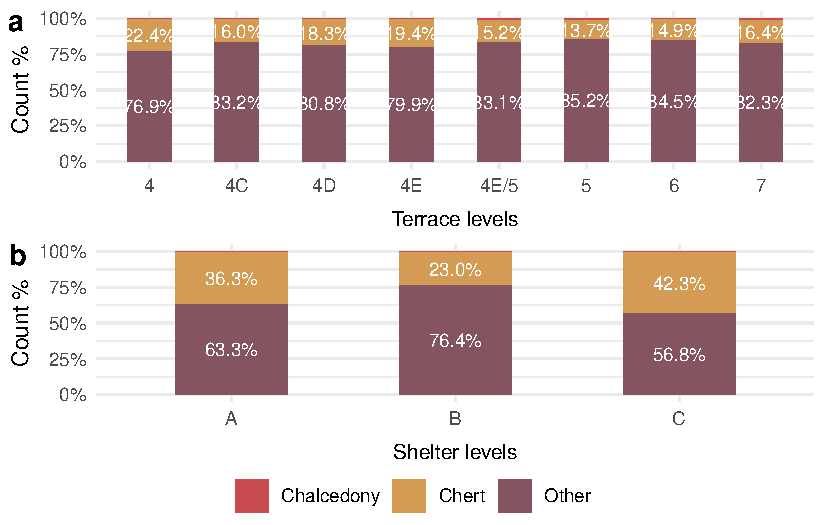
\includegraphics{article2_files/figure-pdf/fig-rm-comparison-1.pdf}

}

\caption{\label{fig-rm-comparison}Comparison of chert, chalcedony, and
other raw materials piece plotted in the Terrace (a) and Shelter (b)
areas of Vale Boi.}

\end{figure}%

We employed both macroscopic and petrographic methods to achieve a more
comprehensive characterization of the materials, aiming to offset the
inherent limitations of each method (Luedtke 1992).

Macroscopic analysis, while revealing several limitations related to the
absence of quantitative variables (Bustillo et al. 2009), proved to be
advantageous given the extensive sample size of chalcedony and chert
lithics under examination (n=4458). The distinct features of various
local cherts facilitate their differentiation from cherts of
neighbouring origins. Consequently, a macroscopic approach offered a
non-destructive, efficient, and cost-effective method for characterizing
all materials (Bustillo et al. 2009; Tarriño and Terradas 2013).
Therefore, we implemented an initial phase of macroscopic analysis,
subsequently augmented by petrographic study to diminish the
subjectivity of the analysis and enhance the material characterization
with petrographic data. The synergistic application of these two methods
has been previously validated in the characterization of Algarve region
cherts, following recent geological survey efforts (Belmiro, Terradas,
and Cascalheira 2023). Hence, an extensive macroscopic and petrographic
collection was already available for comparative analysis with
archaeological materials, employing consistent methodologies. This
reference collection is the Lusolit lithotheque, hosted physically at
ICArEHB (University of Algarve, Faro) and digitally at
www.lusolit.icarehb.com, and aided in the characterization and source
attribution of cherts.

Hand samples were used throughout the macroscopic characterization for
comparison with the archaeological materials, and the archaeological
thin sections were compared with the previously studied geological chert
thin sections. To identify the source of other lithologies which are not
congruent with the regional cherts and identify possible long-distance
chert procurement, we used hand samples and thin sections of cherts from
central Portugal also available in the Lusolit lithotheque. The
lithotheque from the Unit of Geoarchaeology and Archaeometry Applied to
Historic Artistic and Monumental Heritage from the University of Cadiz
(UCA) was also visited to understand the macroscopic variability of the
local and regional cherts of the lower Guadalquivir basin, within the
Atlantic strip of southwestern Spain (present-day provinces of Huelva
and Cádiz).

Following previous studies, we classify the distance of chert sources
from the site as local (1-30 km from the site), regional (30-120 km),
and long-distance (\textgreater120 km) (Herrero-Alonso, Fuertes-Prieto,
and Neira-Campos 2020; Tarriño, Elorrieta, and García-Rojas 2015).

The macroscopic analysis of the archaeological materials was divided
into two steps. The first step included a preliminary characterization
using a hand lens of 10x magnification. This step allowed us to create
types and subtypes based on similar macroscopic characteristics
frequently acknowledged to be useful to describe and discern between
different types of chert; these included characteristics such as colour,
translucency, and feel (Luedtke 1992)-the complete data dictionary for
the recorded variables can be found in the Supplementary Information
(Online Resource 1). In the second step, we used a Nikon SMZ25
stereomicroscope to observe each sample in further detail, which allowed
us to better characterize the artefacts (especially regarding inclusions
and alterations), and the previously established types - the data
dictionary used for the individual samples can also be found in the
Supplementary Information (Online Resource 1). Given the inherent
macroscopic variability of the geological samples and archaeological
specimens, as well as the number of samples, the database used for the
individual analysis was simplified and focused on collecting data
related to weight, cortex, and alterations. This first step was applied
to a total of 4458 artefacts: a sample of 3627 chert artefacts from the
UP sequence of the Terrace area (levels 7 to 4) and 831 chert artefacts
from the Solutrean sequence of the Shelter area (layers A, B, C; all
samples without an attributed layer on the database were excluded from
the analysis).

While the advantages of employing a macroscopic methodology for
analysing the cherts of Vale Boi are notable, a limitation of this
approach is its inability to unequivocally characterize and categorize
artefacts that exhibit surface alterations typical of an open-air site,
including those related to fire, since weathered and altered surface may
destroy visible structures and even alter the chemical composition
(Delluniversità et al. 2019). Other studies frequently exclude samples
that display intense fire damage or several surface alterations
(Delluniversità et al. 2019; Gómez de Soler et al. 2020; Soto 2016). For
the present study, whenever artefacts displayed extensive alterations
and could not be unequivocally characterized
(Figure~\ref{fig-terrace-alterations}), and given the inexistence of a
reference collection for local altered cherts, they were analysed using
the individual sample dataset (Online Resource 1) but grouped in a
category of indeterminate cherts (INDET). This category included key
alterations such as heat/fire-related alterations which clearly impacted
the macroscopic characteristics of the samples, fully changing its
color, luster and texture, and covering them in crazings (e.g.,
Figure~\ref{fig-terrace-alterations} a). Similarly, it also included
alteration rinds that extended through most of the sample, impeding the
identification of its original colour, texture, translucency, inclusions
and fossils (e.g., Figure~\ref{fig-terrace-alterations} b) and the
presence of extended pitting. However, whenever surface alterations were
present in only a limited area of the sample leaving recognizable
macroscopic features and fossils, or when key elements were
distinguishable to make a characterization (e.g., reddening in the Type
2 cherts, Online Resource 2, figure s5), the samples were not collapsed
into the INDET category.

As seen in Table~\ref{tbl-indet-freq}, level 4 shows the highest
percentages of indeterminate artefacts, corresponding to
\textasciitilde40\% of the total sample (n=1037). This is due to the
frequent alterations of the artifacts, especially related to patinas and
alteration rinds, pits, and fire/heat alterations. For all other levels
in the Terrace, indeterminate represents on average \textasciitilde28\%
of the chert artefacts, while in the Shelter the frequency of INDET is
slightly lower (\textasciitilde20-25\%).

\begin{figure}

\centering{

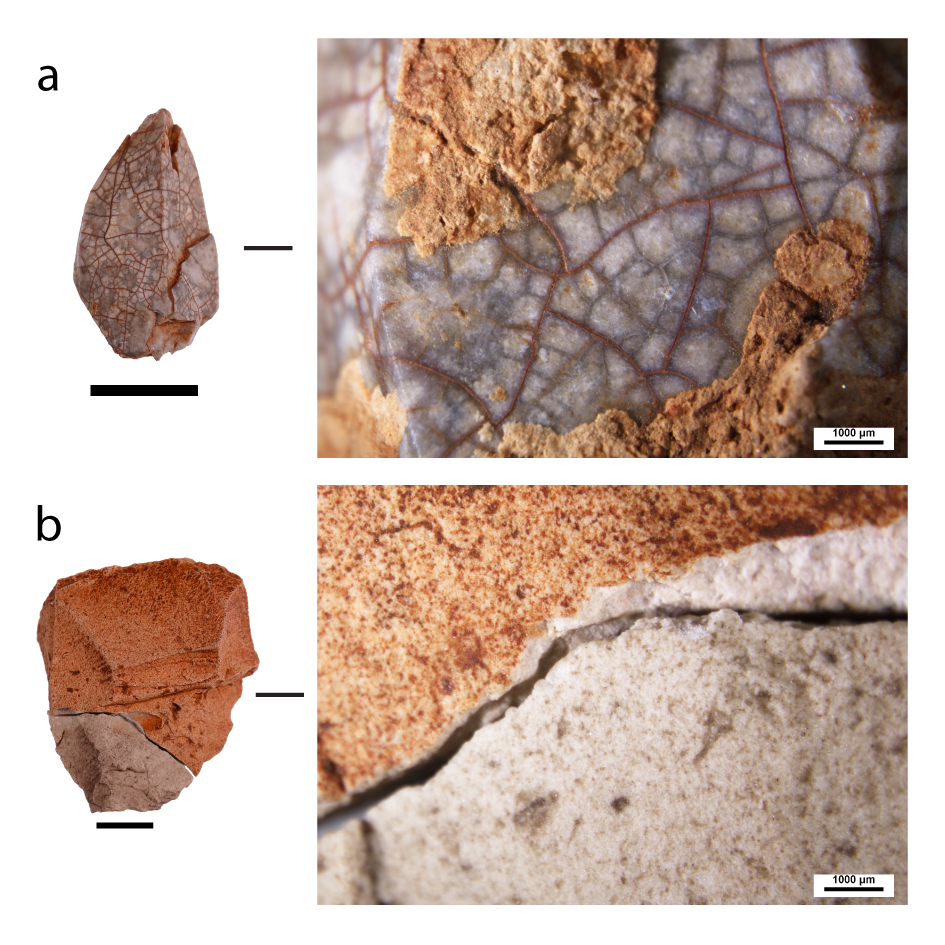
\includegraphics{figures/within-and-beyond/terrace_alterations.png}

}

\caption{\label{fig-terrace-alterations}Samples with extensive
alterations which prevented the identification of chert type. a)
artefact with cracks, white patina and reddening covering 100\% of the
surface; b) artefact with surface alterations, displaying a portion with
patina (brown) and a portion without patina (grey), cleaned with
Hydrochloric acid.}

\end{figure}%

\begin{longtable}[]{@{}
  >{\raggedright\arraybackslash}p{(\columnwidth - 22\tabcolsep) * \real{0.0828}}
  >{\raggedright\arraybackslash}p{(\columnwidth - 22\tabcolsep) * \real{0.0947}}
  >{\raggedright\arraybackslash}p{(\columnwidth - 22\tabcolsep) * \real{0.0828}}
  >{\raggedright\arraybackslash}p{(\columnwidth - 22\tabcolsep) * \real{0.0828}}
  >{\raggedright\arraybackslash}p{(\columnwidth - 22\tabcolsep) * \real{0.0828}}
  >{\raggedright\arraybackslash}p{(\columnwidth - 22\tabcolsep) * \real{0.0828}}
  >{\raggedright\arraybackslash}p{(\columnwidth - 22\tabcolsep) * \real{0.0828}}
  >{\raggedright\arraybackslash}p{(\columnwidth - 22\tabcolsep) * \real{0.0828}}
  >{\raggedright\arraybackslash}p{(\columnwidth - 22\tabcolsep) * \real{0.0828}}
  >{\raggedright\arraybackslash}p{(\columnwidth - 22\tabcolsep) * \real{0.0769}}
  >{\raggedright\arraybackslash}p{(\columnwidth - 22\tabcolsep) * \real{0.0828}}
  >{\raggedright\arraybackslash}p{(\columnwidth - 22\tabcolsep) * \real{0.0828}}@{}}

\caption{\label{tbl-indet-freq}Number and percentage of grouped and
indeterminate (INDET) artefacts by level in the Terrace (levels 4 to 7)
and Shelter (A to C) areas.}

\tabularnewline

\toprule\noalign{}
\begin{minipage}[b]{\linewidth}\raggedright
Group
\end{minipage} & \begin{minipage}[b]{\linewidth}\raggedright
4
\end{minipage} & \begin{minipage}[b]{\linewidth}\raggedright
4C
\end{minipage} & \begin{minipage}[b]{\linewidth}\raggedright
4D
\end{minipage} & \begin{minipage}[b]{\linewidth}\raggedright
4E
\end{minipage} & \begin{minipage}[b]{\linewidth}\raggedright
4E/5
\end{minipage} & \begin{minipage}[b]{\linewidth}\raggedright
5
\end{minipage} & \begin{minipage}[b]{\linewidth}\raggedright
6
\end{minipage} & \begin{minipage}[b]{\linewidth}\raggedright
7
\end{minipage} & \begin{minipage}[b]{\linewidth}\raggedright
A
\end{minipage} & \begin{minipage}[b]{\linewidth}\raggedright
B
\end{minipage} & \begin{minipage}[b]{\linewidth}\raggedright
C
\end{minipage} \\
\midrule\noalign{}
\endhead
\bottomrule\noalign{}
\endlastfoot
Grouped & 619 (59.69\%) & 287 (71.75\%) & 287 (66.74\%) & 332 (73.45\%)
& 155 (73.11\%) & 211 (71.04\%) & 434 (73.06\%) & 149 (72.68\%) & 72
(72.73\%) & 212 (69.28\%) & 349 (81.92\%) \\
Indeterminate & 418 (40.31\%) & 113 (28.25\%) & 143 (33.26\%) & 120
(26.55\%) & 57 (26.89\%) & 86 (28.96\%) & 160 (26.94\%) & 56 (27.32\%) &
27 (27.27\%) & 94 (30.72\%) & 77 (18.08\%) \\
Total & 1,037 (100.00\%) & 400 (100.00\%) & 430 (100.00\%) & 452
(100.00\%) & 212 (100.00\%) & 297 (100.00\%) & 594 (100.00\%) & 205
(100.00\%) & 99 (100.00\%) & 306 (100.00\%) & 426 (100.00\%) \\

\end{longtable}

As previously mentioned, the macroscopic study was followed by a
petrographic approach. To better characterize the different chert types
identified in the macroscopic analysis and aid in minimizing the
inherent caveats of macroscopic methods, 22 thin sections were prepared
at the Thin Section Lab (Toul, France). The samples chosen for this
analysis include at least one sample from each type present throughout
the stratigraphy of the Terrace area, from different archaeological
levels (Table~\ref{tbl-TS-list}). For types that showed high macroscopic
variability (e.g.~translucency and colour variation or differentiated
bioclast facies), thin sections from sub-types were analysed to collect
petrographic data that could reflect this variability. Petrographic thin
sections were analysed by polarized light microscopy (Nikon LV100ND) to
determine the mineral composition, textural characteristics, allochems,
and bioclasts, as well as any other alterations.

\begin{longtable}[]{@{}
  >{\raggedright\arraybackslash}p{(\columnwidth - 6\tabcolsep) * \real{0.0808}}
  >{\raggedright\arraybackslash}p{(\columnwidth - 6\tabcolsep) * \real{0.1010}}
  >{\raggedright\arraybackslash}p{(\columnwidth - 6\tabcolsep) * \real{0.0606}}
  >{\raggedright\arraybackslash}p{(\columnwidth - 6\tabcolsep) * \real{0.7576}}@{}}

\caption{\label{tbl-TS-list}List of archaeological thin sections, with
the summarised description of observed macroscopic variability and
sub-types.}

\tabularnewline

\toprule\noalign{}
\begin{minipage}[b]{\linewidth}\raggedright
Type
\end{minipage} & \begin{minipage}[b]{\linewidth}\raggedright
Sample ID
\end{minipage} & \begin{minipage}[b]{\linewidth}\raggedright
Level
\end{minipage} & \begin{minipage}[b]{\linewidth}\raggedright
Macroscopic variability/sub-type description.
\end{minipage} \\
\midrule\noalign{}
\endhead
\bottomrule\noalign{}
\endlastfoot
Type 1 & I19-1615 & 4D & - \\
Type 2 & I19-2835 & 5 & - \\
Type 2 & H18-1938 & 4D & Type 2 sample with surface alterations. \\
Type 2 & H21-3095 & 4C & Type 2 multi-coloured banding sub-type with
concentration of bioclasts. \\
Type 2 & H21-4234 & 5 & Type 2 multi-coloured banding sub-type without
concentration of bioclasts. \\
Type 2 & H19-2426 & 4D & Type 2 sample with reddening and possible
heat-related alterations. \\
Type 2 & I19-2226 & 4E & Type 2 sample with large iron oxides and rare
sponge spicules. \\
Type 3 & I20-3160 & 5 & - \\
Type 4 & H20-2441 & 4E & - \\
Type 5 & I21-3252 & 4E & - \\
Type 5 & H18-2708 & 5 & Type 5 banding sub-type. \\
Type 6 & I19-3350 & 6 & Type 6 sample with light white patination. \\
Type 6 & I20-3689 & 6 & - \\
Type 6 & J18-778 & 5 & Type 6 with thick white patination. \\
Type 6 & I20-3951 & 6 & Type 6 light brown with opaque white exterior
sub-type. \\
Type 6 & H19-4074 & 6 & Type 6 with lamination and white broad mottling
sub-type. \\
Type 7 & L19-64 & 5 & Type 7 with sponge spicule (01a) and peloidal
(01b) facies. \\
Type 7 & J18-1264 & 8 & Type 7 with peloidal/oolitic (04) facies. \\
Type 8 & H19-2924 & 4E & - \\
Type 9 & I21-2966 & 4C & - \\
Type 10 & H19-4216 & 6 & - \\
INDET & H20-4166 & 6 & Sample with thick white patination. \\

\end{longtable}

The complete petrographic analysis for all thin sections studied in this
paper (including macroscopic and microscopic figures) can be found at
our online research compendium (https://doi.org/10.17605/OSF.IO/DBFT2).
A detailed macroscopic and petrographic description and figures for each
type and sub-type of chert and chalcedony (Online Resource 2) and the
data dictionary used for the petrographic analysis (Online Resource 1)
can be found in Supplementary Information. The complete set of images of
the geological thin sections can also be consulted in the LusoLit online
database.

The entirety of the R code used for the analysis, datasets, and visual
representations contained in this paper can be accessed through our
online research compendium. We used the rrtools package by Marwick et
al. (2018) to create a research compendium and write a reproducible
journal article. The provided files include the complete set of raw data
used in the analysis, along with a custom R project (Wickham 2015)
containing the code required to generate all tables and figures. To
enable maximum reuse, the code is made available under the MIT license,
data under CC‐0, and figures under CC‐BY (additional details can be
found in Marwick 2017).

\section{Results}\label{results-1}

\subsection{Characterization and source
attribution}\label{characterization-and-source-attribution}

Through the macroscopic and petrographic analysis, we identified 10 main
chert/chalcedony types, present throughout the stratigraphy in the
Terrace and Shelter areas (a summarised characterization table can be
found in the Supplementary Information, Online Resource 3). A distinct
type (Type 11) was identified exclusively in the Shelter area, with only
a limited presence in the Terrace (n=2), and 16 varieties, each
consisting of one to three samples, were identified across various
levels of both the Terrace and Shelter. The latter were clustered into a
category named Trace Lithotypes (TL). Through the comparison with the
reference collections, we identified cherts congruent with the local
sources and cherts that are likely not local due to significant
differences in appearance, fossil content, and petrography when compared
to the cherts available in the geological setting located within a 30 km
radius of Vale Boi. Table~\ref{tbl-type-source} shows the different
types of identified cherts and possible sources whenever attribution was
possible.

\begin{longtable}[]{@{}
  >{\raggedright\arraybackslash}p{(\columnwidth - 4\tabcolsep) * \real{0.1358}}
  >{\raggedright\arraybackslash}p{(\columnwidth - 4\tabcolsep) * \real{0.6049}}
  >{\raggedright\arraybackslash}p{(\columnwidth - 4\tabcolsep) * \real{0.2593}}@{}}

\caption{\label{tbl-type-source}Chert types identified during the
analysis, and potential sources. The distance column refers to the
distance of the potential source from Vale Boi, as the crow flies. Only
the TL samples with possible identified sources were included in the
table.}

\tabularnewline

\toprule\noalign{}
\begin{minipage}[b]{\linewidth}\raggedright
Chert type
\end{minipage} & \begin{minipage}[b]{\linewidth}\raggedright
Potential source
\end{minipage} & \begin{minipage}[b]{\linewidth}\raggedright
Distance from source
\end{minipage} \\
\midrule\noalign{}
\endhead
\bottomrule\noalign{}
\endlastfoot
Type 1 & Triassic volcanic formations & \textless10 km \\
Type 2-5 & Lower Carixian formations, southwestern Portugal &
\textless20 km \\
Type 6 & Upper Cretaceous formations, central Portugal &
\textasciitilde215-250 km \\
Type 7 & Betic Systems, southern Spain & \textasciitilde250 km \\
Type 8 & - & - \\
Type 9 & Betic Systems, southern Spain & \textasciitilde250 km \\
Type 10 & - & - \\
Type 11 & - & - \\
TL01 & South Portuguese Zone, southern/central Portugal &
\textgreater100 km \\
TL10-11 & Upper Cretaceous formations, central Portugal &
\textasciitilde215-250 km \\
TL15-16 & Betic Systems, southern Spain & \textasciitilde250 km \\

\end{longtable}

\subsubsection{Cherts congruent with local sources (Types
1-5)}\label{cherts-congruent-with-local-sources-types-1-5}

The raw materials which are congruent with local sources are the
chalcedony and massive, micro-cryptocrystalline cherts
(Figure~\ref{fig-local-types}). The chalcedony (Type 1;
Figure~\ref{fig-local-types} a) is identified as a massive, fibrous
variety without allochems (Figure~\ref{fig-local-types} a2). It
represents 6.6\% of the overall Terrace cherts (excluding INDET) and
2.6\% in the Shelter. It presents a colourless and translucent
appearance, frequently exhibiting partial or complete white patination
(Figure~\ref{fig-local-types} a1). This type is marked by extensive
crystallizations, irregularities, and fractures, coupled with
post-depositional alterations that challenge the identification and
preservation of the cortex. Both macroscopic and petrographic analyses
confirm its congruence with hydrothermal chalcedony located within
lenses in Triassic volcanic formations, in the known outcrops of Monte
do Tolo, Taboal and Cerro Velho (\textless10 km west of Vale Boi, as the
crow flies; Figure~\ref{fig-map} b), which are similarly marked by
irregularities and fractures.

The cherts are massive micro-cryptocrystalline quartz from a marine
environment (Figure~\ref{fig-local-types} b-h). They represent
\textasciitilde60\% of the overall Terrace cherts and
\textasciitilde80\% of the chert in the Shelter. Macroscopically, these
types show variability which resulted in their separation in four
different macroscopic types (Type 2 to 5). In general, these are opaque
to sub-translucent cherts, with colours varying from brown, yellow, pale
red, and grey, with the frequent presence of spicules and iron oxides.
The differences are in their colours, nodule morphology, frequency, and
variety of bioclasts (Type 2 including triaxon sponge spicules and
echinoderm spines), something already identified in the geological
samples (Belmiro, Terradas, and Cascalheira 2023). As seen in table
Table~\ref{tbl-cortex_tab}, whenever present, the cortex seems to show a
mixture of irregular cortex and rounded cortex, both from an outcrop
source. Petrographically, however, these cherts are homogeneous, except
for a small number of artefacts with a banded variety within Type 5.
These cherts are characterized by wackestone textures, with accessory
amounts of macrocrystalline quartz and fibrous chalcedony, frequently
found replacing fossils and occasionally dolomite. Type 5 shows higher
percentages of micrite/sparite. In all samples, fossils range from
common to very frequent, albeit frequently unidentifiable. When
identifiable in thin section, they are sponge spicules
(Figure~\ref{fig-local-types} b2, c2, h2), with the rare occurrence of
possible foraminifera (Type 2 and Type 5) and ostracod
(Figure~\ref{fig-local-types} h3) in a sample from Type 5. Porosity
varies between 10\% and 1\%, of vug type. Despite the petrographic
homogeneity between local types, this macroscopic separation was
maintained for its possible usefulness in identifying preferred types of
nodules or macroscopic varieties through time and for future correlation
with technological data.

\begin{table}

\caption{\label{tbl-cortex_tab}Frequency of cortex type and thickness by
raw material from the Terrace area, characterized during the individual
analysis of the lithic assemblage.}

\centering{

\fontsize{12.0pt}{14.4pt}\selectfont
\begin{tabular*}{\linewidth}{@{\extracolsep{\fill}}lccccccccccc}
\toprule
\textbf{Variable} & \textbf{TYPE 1}  N = 8\textsuperscript{\textit{1}} & \textbf{TYPE 2}  N = 267\textsuperscript{\textit{1}} & \textbf{TYPE 3}  N = 138\textsuperscript{\textit{1}} & \textbf{TYPE 4}  N = 112\textsuperscript{\textit{1}} & \textbf{TYPE 5}  N = 134\textsuperscript{\textit{1}} & \textbf{TYPE 6}  N = 163\textsuperscript{\textit{1}} & \textbf{TYPE 7}  N = 108\textsuperscript{\textit{1}} & \textbf{TYPE 8}  N = 19\textsuperscript{\textit{1}} & \textbf{TYPE 9}  N = 18\textsuperscript{\textit{1}} & \textbf{TYPE 10}  N = 3\textsuperscript{\textit{1}} & \textbf{TL}  N = 3\textsuperscript{\textit{1}} \\ 
\midrule\addlinespace[2.5pt]
{\bfseries Cortex type} &  &  &  &  &  &  &  &  &  &  &  \\ 
    Irregular & 1 (13\%) & 74 (28\%) & 52 (38\%) & 50 (45\%) & 31 (23\%) & 20 (12\%) & 30 (28\%) & 2 (11\%) & 0 (0\%) & 0 (0\%) & 0 (0\%) \\ 
    Rounded & 1 (13\%) & 118 (44\%) & 53 (38\%) & 35 (31\%) & 69 (51\%) & 116 (71\%) & 46 (43\%) & 14 (74\%) & 14 (78\%) & 1 (33\%) & 3 (100\%) \\ 
    Pebble & 0 (0\%) & 4 (1.5\%) & 2 (1.4\%) & 0 (0\%) & 2 (1.5\%) & 6 (3.7\%) & 1 (0.9\%) & 0 (0\%) & 0 (0\%) & 0 (0\%) & 0 (0\%) \\ 
    Indeterminate & 6 (75\%) & 71 (27\%) & 31 (22\%) & 27 (24\%) & 32 (24\%) & 21 (13\%) & 31 (29\%) & 3 (16\%) & 4 (22\%) & 2 (67\%) & 0 (0\%) \\ 
{\bfseries Thickness} &  &  &  &  &  &  &  &  &  &  &  \\ 
    Thin & 7 (88\%) & 121 (45\%) & 49 (36\%) & 24 (21\%) & 105 (78\%) & 151 (93\%) & 37 (34\%) & 13 (68\%) & 13 (72\%) & 0 (0\%) & 3 (100\%) \\ 
    Medium & 1 (13\%) & 122 (46\%) & 77 (56\%) & 53 (47\%) & 23 (17\%) & 10 (6.1\%) & 51 (47\%) & 5 (26\%) & 3 (17\%) & 3 (100\%) & 0 (0\%) \\ 
    Thick & 0 (0\%) & 24 (9.0\%) & 12 (8.7\%) & 35 (31\%) & 6 (4.5\%) & 2 (1.2\%) & 20 (19\%) & 1 (5.3\%) & 2 (11\%) & 0 (0\%) & 0 (0\%) \\ 
\bottomrule
\end{tabular*}
\begin{minipage}{\linewidth}
\textsuperscript{\textit{1}}n (\%)\\
\end{minipage}

}

\end{table}%

Based on the previously described macroscopic and petrographic
characteristics of the Lower Jurassic cherts of the Algarve (Belmiro,
Terradas, and Cascalheira 2023), we interpret Types 2, 3, 4, and 5 to be
local, as they are congruent with the described characteristics
representative of cherts from the Lower Jurassic found in the known
outcrops Cabo S. Vicente, Foz dos Fornos, Ponta dos Altos, Praia do
Belixe and Ferrel (Carixian; \textless20 km from Vale Boi, as the crow
flies), possibly Upper Jurassic Kimmeridgian outcrops of Mareta
(\textasciitilde15 km from Vale Boi, as the crow flies) and Middle
Jurassic Malhão formations (80-100 km east of Vale Boi, as the crow
flies) of the Algarve basin. Types 2 and 3 are congruent with the
frequently available brown/yellow and red nodules and beds
(Figure~\ref{fig-local-types} b-d), ranging from uncommon to very
frequent fossils. These can be found in all previously mentioned
outcrops. The macroscopic similarities of Types 4 and 5 are more limited
(Figure~\ref{fig-local-types} e-h), as they show similarities to
specific nodules, rarely found in the known outcrops, and mostly located
in the inland Lower Jurassic outcrop of Ferrel (Figure~\ref{fig-map} b).
As such, we interpret these cherts as local, but possibly from nodules
and inland outcrops that are no longer frequently available or visible
in the landscape. This is especially relevant since the inland outcrops
of Ferrel are currently mostly destroyed and can be found in poor
preservation conditions, due to recent human intervention and
construction work, and with small, broken nodules in the surface,
frequently altered (Belmiro, Terradas, and Cascalheira 2023).

\begin{figure}

\centering{

\includegraphics{figures/within-and-beyond/local_grid.png}

}

\caption{\label{fig-local-types}Variability of local chert types and
main petrographic characteristics. a) Type 1 macroscopic and microscopic
views: a1) macroscopic view with a stereomicroscope of white patina and
fractures; a2) microscopic view of thin section (XPL), with visible
fibrous chalcedony composition and without allochems. b) Type 3
macroscopic and microscopic views: b1) macroscopic view with a
stereomicroscope of iron oxides and unidentifiable fossils; b2)
microscopic view of thin section (XPL), with visible unidentifiable
fossils and iron oxides. c-d) Type 2 macroscopic and microscopic views
of multicoloured (c) and single-colour (d) varieties. c1) macroscopic
view with a stereomicroscope of the multicoloured bands with iron oxides
and unidentifiable fossils; d1) macroscopic view with a stereomicroscope
of iron oxides and unidentifiable fossils; c2) microscopic view of thin
section (PPL), with visible unidentifiable fossils, sponge spicules and
iron oxides; d2) microscopic view of thin section (XPL), with visible
unidentifiable fossils and iron oxides. e-f) Type 4 macroscopic and
microscopic views: e) macroscopic view with a stereomicroscope of
unidentifiable fossils and white splotches; f1) macroscopic view with a
stereomicroscope of iron oxides and unidentifiable fossils within white
and yellow splotches; f2) microscopic view of thin section (XPL), with
visible unidentifiable fossils and iron oxides; f3) microscopic view of
thin section (PPL) with a concentration of fossils (possibly sponge
spicules) and a fracture. g-h) Type 5 macroscopic and microscopic views:
g) macroscopic view with a stereomicroscope; h1) macroscopic view with a
stereomicroscope with visible unidentifiable fossils; h2) microscopic
view of thin section (PPL), with visible unidentifiable fossils, sponge
spicules and iron oxides; h3) microscopic view of thin section (XPL)
with small unidentifiable fossils, iron oxides and a possible ostracod
replaced by fibrous chalcedony and macrocrystalline quartz.}

\end{figure}%

\subsubsection{Cherts not congruent with local sources (Types 6-11 and
TL)}\label{cherts-not-congruent-with-local-sources-types-6-11-and-tl}

We identified six chert types with macroscopic and petrographic
characteristics that are not congruent with the chert available in known
outcrops in western Algarve (Figure~\ref{fig-distance-types}).

\begin{figure}

\centering{

\includegraphics{figures/within-and-beyond/nonlocal_grid.png}

}

\caption{\label{fig-distance-types}Variability of non-local types and
main petrographic characteristics. a-b) Type 6 macroscopic and
microscopic views: a1) macroscopic view with a stereomicroscope with a
small degree of white patina and no visible fossils; b1) macroscopic
view with a stereomicroscope of a thick alteration rind but translucent
interior where some unidentifiable fossils are visible; a2) microscopic
view of thin section (PPL) with a mudstone texture; b2) microscopic of
thin section (XPL) with small unidentifiable fossils and a laminar
microstructure. c-d) Type 7 macroscopic and microscopic views of the
peloidal facies (c) and oolitic facies (d): c1) macroscopic view with a
stereomicroscope of peloids and sponge spicules; d1) macroscopic view
with a stereomicroscope of poorly preserved ooids; c2) microscopic view
of thin section (PPL) with packstone texture composed mainly of peloids;
d2) microscopic view of thin section (PPL) with packstone texture
composed mainly of ooids. e-f) Type 8 macroscopic and microscopic views,
with foraminifera represented by the white and black arrows: e)
macroscopic view with a stereomicroscope with abundant unidentifiable
fossils and foraminifera; f1) macroscopic view with a stereomicroscope
with abundant unidentifiable fossils but no visible foraminifera; f2)
microscopic view of thin section (PPL) with packstone texture composed
of unidentifiable fossils and foraminifera which are not visible
macroscopically; f3) microscopic view of thin section (PPL) with
packstone texture composed of unidentifiable fossils and foraminifera
which not are visible macroscopically. g) Type 9 macroscopic and
microscopic views: g1) macroscopic view with a stereomicroscope of
unidentifiable fossils and two different fabrics; g2) microscopic view
of thin section (XPL) with packstone texture composed of concentrations
of unidentifiable fossils and opaques which create a banded
microstructure. h) Type 10 macroscopic and microscopic views: h1)
macroscopic view with a stereomicroscope of ooids and fractures filled
with chalcedony; h2) microscopic view of thin section (PPL) with
packstone texture composed of ooids with different levels of
preservation.}

\end{figure}%

Type 6 (Figure~\ref{fig-distance-types} a-b) corresponds to a massive
cryptocrystalline quartz with a mudstone texture, from a marine
environment. It represents \textasciitilde18\% of the overall Terrace
cherts and \textasciitilde12\% of the chert in the Shelter. This chert
is translucent and shows a variety of colours, ranging from brown, red,
and grey, which seem to vary in function of the artefact's thickness. In
unaltered samples, visible bioclasts are rare. The cortex is mostly
rounded, and rarely pebble-like, ranging from thin to medium thickness
(Table~\ref{tbl-cortex_tab}). Two sub-types were individualized based on
macroscopic characteristics such as colour, translucency variation, and
patterns, although they may simply reflect the use of specific nodules
from within Type 6's variability. Five thin sections were produced to
better characterize the macroscopic variability of this type and
sub-types. The petrographic analysis shows the samples are characterized
by a massive microstructure, mainly composed of cryptocrystalline quartz
(between 95-97\% in the samples), with accessory fibrous chalcedony
found replacing fossils or filling fractures
(Figure~\ref{fig-distance-types} a2-b2), and in some samples
macrocrystalline quartz, microcrystalline quartz, and micrite/sparite.
Allochems are opaques, iron oxides, and bioclasts. Bioclasts are
unidentifiable and poorly preserved, with rare identifiable fossils such
as sponge spicules, replaced by fibrous chalcedony and rarely by
microcrystalline quartz. Porosity is present between \textless1-1\%, of
vug-type when identifiable.

The similarities between chert artefacts at the UP occupations of Vale
Boi and the chert from the Rio Maior region (central Portugal;
Figure~\ref{fig-map} a) have been previously suggested although without
systematic studies to ascertain the attribution (Nuno Bicho et al. 2013;
Pereira, Bicho, et al. 2016). These Cretaceous cherts, mostly found in
secondary deposition settings, are described as frequently translucent,
with geodes, colours ranging from yellow to red or grey, and
mineralogically homogeneous between them. Petrographic studies from
central Portugal highlight the presence of iron oxide accumulations and
rare fossil ghosts or frequently difficult to see in thin section
(Matias 2016). When identified, sponge spicules and possible rare
foraminifera have been identified (Matias 2012).

Studies of Upper Cretaceous cherts located in the Lisbon area describe
cherts with similar macroscopic characteristics (Figure~\ref{fig-map}
a), with micro-cryptocrystalline quartz mudstones with bioclasts such as
sponge spicules or bivalve fragments, or wackestone/packstone textures
with abundant bioclasts, including ostracods and different types of
foraminifers (Jordão and Pimentel 2022). These cherts have also been
reported as found in highly variable cobble morphologies and macroscopic
traits, which is also observable through the reference samples from
central Portugal hosted at LusoLit. Similar to the archaeological thin
sections from Type 6 and congruent with other studies (Jordão and
Pimentel 2022; Matias 2016), the thin sections produced from the
Cretaceous cherts hosted at Lusolit show a massive, cryptocrystalline
mudstone structure, with uncommon fossils (ghosts), iron oxides and low
porosity (\textless1\%). From these Cretaceous cherts from central
Portugal, only the dark grey nodules (sample RT231, with petrographic
descriptions available in our online research compendium) showed
identifiable fossils which were rare ostracods.

Based on the macroscopic and petrographic similarities to the geological
references from central Portugal and congruence with previous studies
from this area, we interpreted Type 6 (and sub-types) as belonging to
the macroscopically variable Cretaceous cherts (Upper Cenomanian
formations) from central Portugal, between \textasciitilde215-250 km (as
the crow flies) north of Vale Boi (Figure~\ref{fig-map} a).

Type 7 (Figure~\ref{fig-distance-types} c-d) is a massive
micro-cryptocrystalline, peloidal/oolitic packstone, from a marine
environment and possibly a high-energy, shallow depositional
environment, due to the type, sorting, and preservation conditions of
the ooids. In the terrace, it represents 10\% of the overall Terrace
cherts and less than 1\% of the chert in the Shelter. It is
characterized by white and grey colours. The cortex is from an outcrop,
rounded and in lesser frequencies (\textless30\%) irregular, and varying
between medium thickness to thick (Table~\ref{tbl-cortex_tab}). This
type shows several facies, with different types and concentrations of
allochems and bioclasts, such as peloids
(Figure~\ref{fig-distance-types} c1), ooids
(Figure~\ref{fig-distance-types} d1), and sponge spicules. A detailed
scheme of the facies can be found in the Supplementary Information
(Online Resource 2). The petrography results show this chert has a
massive microstructure and packstone texture
(Figure~\ref{fig-distance-types} c2-d2). It is composed mainly of
micro-cryptocrystalline quartz (80\%), fibrous chalcedony (10\%), and
micrite (10\%). Allochems are opaques, iron oxides, ooids, and peloids.
The ooids are poorly preserved and only uncommonly show concentric
lamellae in plane-polarized light. Unlike macroscopical observations,
bioclasts under the thin section are all unidentifiable, although rare
fossils may be bivalve shells. Porosity is variable (\textless1-10\%).

The consultation of the lithotheque hosted at UCA allowed us to identify
a subset of cherts with similarities to those from Type 7 from the
Middle Subbetic region (Betic Systems, south Spain,
Figure~\ref{fig-map}). These cherts are massive, sub-translucent,
peloidal/oolitic packstones. Allochems include very frequent peloids and
ooids. The peloids are densely arranged in the samples, more or less
visible depending on the alterations to the surface or the thickness.
The ooids are poorly sorted, with oval or round shapes, and replaced by
quartz. Uncommonly the ooids show a preserved nucleus. The presence of
bioclasts varies between samples, ranging between common to rare, and
when present/identifiable include sponge spicules (common), foraminifera
(rare to uncommon), and echinoderm spines (rare). Similar cherts have
also been identified and described in previous works, describing grey
cherts with peloidal and oolitic facies and occasional foraminifera
(Rodríguez, Rodríguez, and Pelegrin 2011). Despite the non-existence of
thin sections for comparison, the macroscopic similarities between the
cherts allow us to interpret Type 7 as coming from the Upper Jurassic
formations of the Betic Systems, located in the south and southeastern
Iberian Peninsula, at least 250 km (as the crow flies) east from Vale
Boi (Figure~\ref{fig-map}).

Type 8 (Figure~\ref{fig-distance-types}, e-f) corresponds to a massive
micro-cryptocrystalline quartz from a marine environment and
shelf/platform depositional environment. It represents
\textasciitilde2\% of the overall Terrace cherts and \textasciitilde5\%
of the chert in the Shelter. Identified and well-preserved fossils are
foraminifera from the Pfenderenidae family
(Figure~\ref{fig-distance-types} e, f2), which are larger benthic
foraminifera from marine environments (BouDagher-Fadel 2008). The
association of these foraminifera indicates this chert formed from
sediments deposited possibly between the Jurassic to the Cretaceous.
Macroscopically, this type is characterized by grey and white colours
(Figure~\ref{fig-distance-types} e-f1). The translucency ranges from
sub-translucent to opaque. Whenever present, the cortex is rounded and
thin (Table~\ref{tbl-cortex_tab}). Petrographically, this type is a
packstone (mudstone texture close to the edges) with a massive
microstructure. It is composed of 97\% micro-cryptocrystalline quartz,
macrocrystalline quartz, and fibrous chalcedony mostly replacing
fossils. Other minerals include uncommon iron oxides and the porosity is
of vug type (3\%). Fossil content is very frequent
(Figure~\ref{fig-distance-types} f2-f3), albeit mostly unidentifiable
and poorly preserved. Identified fossils are rare sponge spicules, rare
ostracods with some degree of preservation, common small, unidentified
foraminifera (100 μm) of differing preservation degrees, and as
mentioned above, foraminifera from the Pfenderenidae family (500 μm).
Despite the macroscopic similarities between type 8 and cherts from the
Middle Subbetic region chert formations (Figure~\ref{fig-map}), the
geological reference samples showed no macroscopically visible
foraminifera. However, our results indicate that despite no foraminifera
being visible macroscopically, they are present in thin section. The
fact that no foraminifera were identified in the small number of
analysed samples from the UCA lithotheque with similarities to Type 8
(n=3) may simply reflect their uncommon visibility, possibly due to
patination. Another possible source for Type 8 cherts may be the Upper
Cretaceous wackestone/packstone cherts with foraminifers from the Lisbon
region (Jordão and Pimentel 2022). However, these studies do not specify
the existence of Pfenderenidae foraminifers. Given the lack of this
specific fossil in the reference samples from the Betic chert
\textasciitilde250 km east and southeast, and the central Portugal
cherts 215-250 km north, the probable source of Type 8 remains unknown.

Type 9 (Figure~\ref{fig-distance-types} g) corresponds to a banded
micro-cryptocrystalline quartz/micrite peloidal packstone. It
corresponds to less than \textasciitilde2\% of the overall cherts in the
Terrace and Shelter areas. It is opaque, has a heterogeneous structure
and is characterized by a variable colour distribution: it shows a
horizontal, finely laminated pattern, with grey dark bands intercalated
with light grey bands (Figure~\ref{fig-distance-types} g1). Whenever
present, the cortex is rounded and is generally thin
(Table~\ref{tbl-cortex_tab}). In specific samples, the cortex is present
on two parallel planes of the sample (parallel to the laminations),
which indicates the chert was originally available in bedded layers.
Petrographically this chert is a banded packstone (banding of
sedimentary origin; Figure~\ref{fig-distance-types} g2), composed mostly
of micro-cryptocrystalline quartz (48\%), micrite (40\%), dolomite
(10\%), and accessory fibrous chalcedony and mica (muscovite). The
allochems are peloids, unidentifiable bioclasts, iron oxides, and opaque
minerals. Porosity is low (1\%). Although its origin is unknown, when
visiting the UCA lithotheque, we identified a small type of banded black
cherts without noticeable fossils or inclusions. Despite the lack of
comparative petrographic data, the macroscopic resemblances raise the
possibility that Type 9 belongs to Betic chert formations in southern
Spain, 250 km east (as the crow flies) from the site
(Figure~\ref{fig-map}).

Type 10 (Figure~\ref{fig-distance-types} h) is an oolitic packstone,
massive micro-cryptocrystalline micrite/quartz from a marine environment
and possibly a high-energy, shallow depositional environment, due to the
type, sorting, and preservation conditions of the ooids. It represents
\textasciitilde1\% of the overall Terrace cherts and less than 0.1\% of
the chert in the Shelter. Its heterogeneous structure has two types of
fabrics with different macroscopic characteristics: brown (opaque) and
black (sub-translucent) fabric (Figure~\ref{fig-distance-types} h1). The
sample chosen for the thin section is composed of 35\%
micro-cryptocrystalline quartz, 53\% micrite, 9\% macrocrystalline
quartz, and accessory fibrous chalcedony (filling fractures) and mica;
the percentages of quartz and micrite might be related to the fabrics
present in the artefacts. Allochems are common iron oxides and very
frequent ooids. Bioclasts are rare, poorly preserved, and replaced by
quartz. The porosity is intraparticle and vug (10\%). The ooids are
distributed homogeneously across the sample (although macroscopically
visible in the brown fabric) and are highly abundant and concentrated.
They are poorly sorted, varying between 500 and 20 μm
(Figure~\ref{fig-distance-types} h2), show round-to-elliptical shapes
and their preservation is variable: some ooids show a poorly preserved
micritic structure, while others show concentric laminae structures
around a round nucleus (Flügel 2010). This chert shows no similarities
to any consulted reference material. Despite the existence of oolitic
limestones in the Algarve region correspondent to Middle and Upper
Jurassic formations and often described as whiteish (Rocha et al.,
1979), the presence of oolitic chert in the region is not recognized in
geological and archaeological literature (Cardoso, Andrade, and Martins
2018; R. Rocha et al. 1979; Verissimo 2004) and the visit of outcrops
mentioned in the geological cartography did not allow their
identification.

Type 11 (Figure~\ref{fig-small-types}) is a banded/laminated mudstone,
characterized by the presence of a conchoidal fracture (within the
nodule) and a non-conchoidal, laminar fracture (at the edges of the
nodule). This chert type is grey, opaque, and without identifiable
allochems. This chert shows a limited presence at the archaeological
site as previously mentioned, restricted to the Solutrean occupations,
and corresponding to less than 0.1\% of the Terrace cherts and
\textasciitilde2\% of Shelter cherts.

\begin{figure}

\centering{

\includegraphics{figures/within-and-beyond/small_grid.png}

}

\caption{\label{fig-small-types}Macroscopic view with a stereomicroscope
of non-local Type 11 and TL cherts. Type 11 -- detail of banded patterns
composed of parallel different fabrics; TL01 -- detail of the jasper and
fractures filled with chalcedony; TL02 -- detail of the chalcedony with
unidentified orange inclusions; TL03 -- detail of two round inclusions,
possibly iron oxides; TL04 - detail of massive chert with fractures
filled with chalcedony; TL05 -- detail of the banded pattern within the
grey mudstone texture; TL06 - detail of the small, finely sorted ooids;
TL07 -- detail of the dendritic laminations, possibly composed of iron
oxides; TL08 -- detail of the mudstone structure, without the presence
of allochems; TL09a/b -- detail of the mossy, orange and red inclusions
within the chalcedony; TL10 -- detail of the speckling and laminated
patterns within the mudstone structure; TL11 -- detail of the banding
within the mudstone structure; TL12 -- detail of the poorly preserved
ooids, only visible under the stereomicroscope; TL13 -- detail of the
bands and laminations within the mudstone texture fabric; TL14 -- detail
of an unidentified benthic foraminifera; TL15 -- detail of the interface
between the massive brown fabric and splotches; TL16 - detail of the of
the massive structure with unidentifiable inclusions.}

\end{figure}%

Finally, the TL types (Figure~\ref{fig-small-types}) are characterized
by several samples without macroscopic correspondence to the previously
identified types or to the local cherts and chalcedony from the Algarve
region previously described by Belmiro et al. (2023). These are composed
mostly of blanks or retouched tools, rarely with cortex
(Table~\ref{tbl-cortex_tab}), and rarely the same TL type is found in
different archaeological layers. A detailed description of these types
can be found in the Supplementary Information (Online Resource 2). In
both areas, the TL cherts compose less than 1\% of the cherts.

Apart from the types common throughout the stratigraphy of the Terrace
and Shelter, Type 11 and samples from the TL type also show no
identifiable source. The exceptions are TL01, TL10-11 and TL15-16.

Jasper is known in the South Portuguese Zone area (Oliveira 1984), from
southern/central Portugal to Spain, north of the Algarve (from Aljustrel
to Beja; Figure~\ref{fig-map}), suggesting that the source of TL01 may
be from south/central Portugal at a minimum distance of 100 km north and
northeast from Vale Boi (as the crow flies).

Similarly, despite being different from the most frequent Cretaceous
nodules, the macroscopic similarities between TL10 and TL11 and specific
nodules from central Portugal in the Lusolit lithotheque may indicate
these cherts are from the Estremadura/Lisbon area (Figure~\ref{fig-map}
a). This difference in appearance may be due to the already-mentioned
variability of the nodule's macroscopic characteristics.

Finally, TL15 and TL16 show macroscopic similarities to radiolarite
reference samples located at the Cadiz lithotheque, which may indicate
the source of these cherts is from the Middle Subbetic region (Domínguez
Bella 2010; Domínguez-Bella 2006).

\subsection{Stratigraphical
distribution}\label{stratigraphical-distribution}

\subsubsection{Terrace area}\label{terrace-area}

Most chert types described above are consistently present across the
Terrace stratigraphy (except for Type 11 which appears only in level 4
and in a small number of artefacts; n=2). However, being ubiquitous, we
identified a difference in the percentages of chert types throughout the
stratigraphy (Figure~\ref{fig-type-per-level}).

In the Gravettian occupations (levels 6 and 7) and at the start of the
Proto-Solutrean (level 5) local cherts make up \textasciitilde45-60\%,
while the combined non-local cherts make up \textasciitilde65-40\%.
Level 6 shows the highest percentages of all non-local chert use, with
specific types like Type 6 representing \textasciitilde30\%, although
when considering the sum of weight, the percentages reduce, and
non-local chert represents \textasciitilde50\% of total chert. The
percentages of local chert increase in the following occupations. In the
Proto-Solutrean (levels 4E and 4E/5) and Solutrean (levels 4, 4C, and
4D) local cherts make up more than \textasciitilde70\% of the sample and
80\% when considering the sum of weight, while non-local cherts decrease
significantly and represent percentages lower than 30\%. Despite the
increase of local cherts during the Proto-Solutrean and Solutrean, there
are still significant differences between the local types present in the
two technocomplexes. During the top Proto-Solutrean occupations the
grey/white cherts (Type 4) are the most present chert with percentages
between 35-20\%, while in the Solutrean levels, the yellow/brown cherts
(Type 2) are present in the highest percentage, at \textasciitilde30\%.

\begin{figure}

\centering{

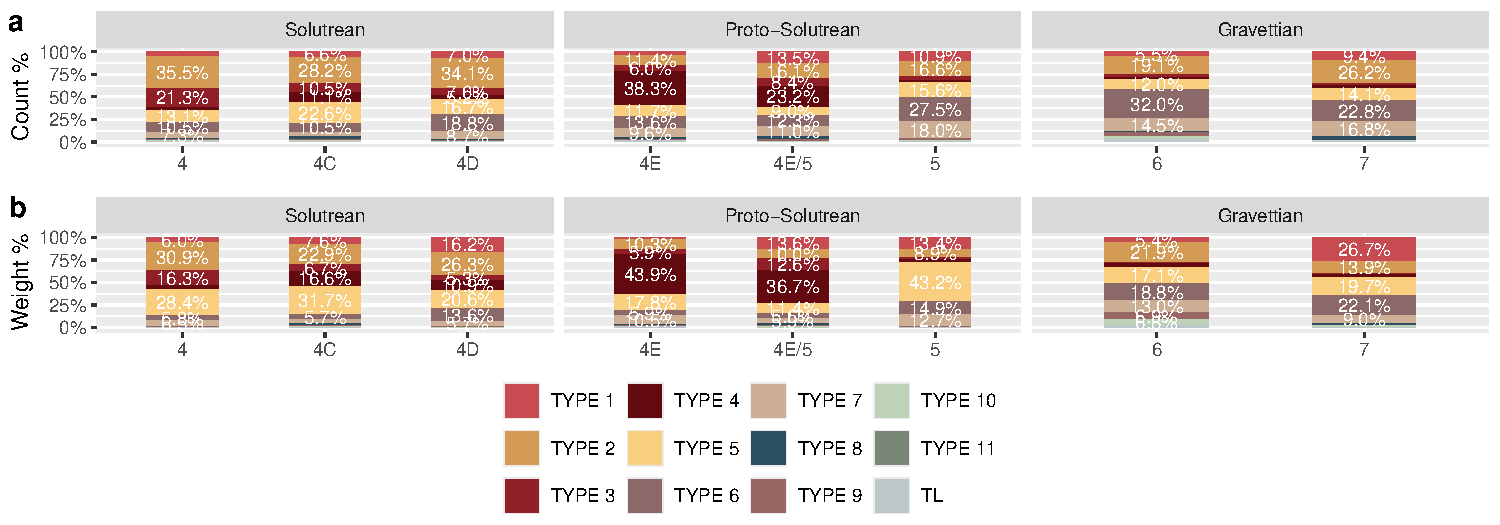
\includegraphics{article2_files/figure-pdf/fig-type-per-level-1.pdf}

}

\caption{\label{fig-type-per-level}Terrace area chalcedony and chert
type frequency (a) and weight sum (b) per level, without unidentifiable
samples. Only percentages superior to the 5\% threshold are shown in the
figure. Type 1 to 5 (yellow and red colours) represent local chalcedony
and cherts. Type 6, 7 and 9 represent non-local cherts with identified
probable provenience (brown colours). Type 8, 10 and 11 represent
non-local cherts with non-identified provenience (blue and green
colours).}

\end{figure}%

When plotting the weight, it is apparent that most of the samples are
located under the 10 gr mark, with median and bottom quartiles often
falling under the 5 gr line (Figure~\ref{fig-weight}). Local types, such
as Type 2, Type 4, and Type 5, although mostly represented by artefacts
with a medium mass (\textasciitilde5-10 gr), show the heaviest and
highest number of heavy artefacts. In comparison, other types, although
showing some variation in the weight of artefacts, show smaller
artefacts and their means and medians are frequently closer to the
bottom quartile. As seen in (Figure~\ref{fig-weight}), non-local types
show larger weights from level 5 to level 7.

\begin{figure}

\centering{

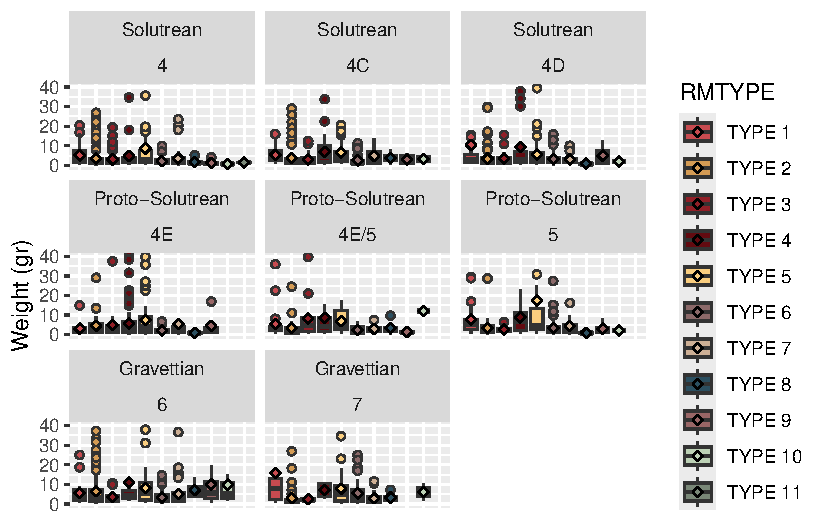
\includegraphics{article2_files/figure-pdf/fig-weight-1.pdf}

}

\caption{\label{fig-weight}Terrace boxplots of chert type weight (gr)
per level. Diamond shape within the boxplots represents weight mean.
Type 1 to 5 (yellow and red colours) represent local chalcedony and
cherts. Type 6, 7 and 9 represent non-local cherts with identified
probable provenience (brown colours). Type 8, 10 and 11 represent
non-local cherts with non-identified provenience (blue and green
colours).}

\end{figure}%

\subsubsection{Shelter area}\label{shelter-area}

The same raw materials found in the Terrace area are also found in the
Solutrean occupation of the Shelter, albeit with some differences
(Figure~\ref{fig-analysis_shelter}). The local cherts make up between
\textasciitilde65-75\% (considering both counts and weight) of the
sample and are mainly composed of the brown/yellow cherts (Type 2) that
frequently characterize the Lower Jurassic outcrops of the Algarve
(Figure~\ref{fig-analysis_shelter} a-b). The presence of cherts not
congruent with the local sources is, like level 4 in the Terrace, close
to 25\%, although dominated mostly by Type 6 (\textasciitilde15\%).
Similarly to the Solutrean occupations of the Terrace, although the
artefacts are generally small (lower weights), the local types show a
higher variability in mass, with several outliers and heavy samples when
compared to the non-local types (Figure~\ref{fig-analysis_shelter} c).

\begin{figure}

\centering{

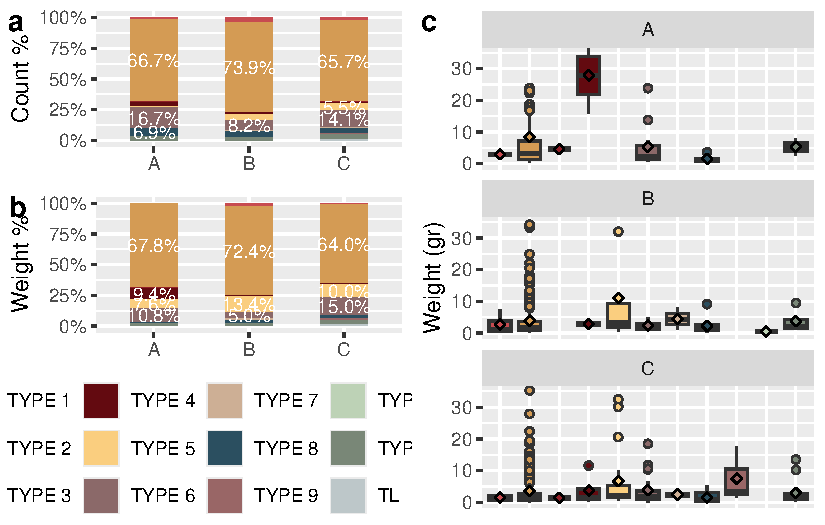
\includegraphics{article2_files/figure-pdf/fig-analysis_shelter-1.pdf}

}

\caption{\label{fig-analysis_shelter}a-b) Shelter area chalcedony and
chert type frequency (a) and weight sum (b) per level, without
unidentifiable samples. Only percentages superior to the 5\% threshold
are shown in the figure. c): Shelter boxplots of chert type weight (gr)
per level. Type 1 to 5 (yellow and red colours) represent local
chalcedony and cherts. Type 6, 7 and 9 represent non-local cherts with
identified probable provenience (brown colours). Type 8, 10 and 11
represent non-local cherts with non-identified provenience (blue and
green colours).}

\end{figure}%

\section{Discussion}\label{discussion-1}

The macroscopic and petrographic analysis of chert and chalcedony lithic
materials from the UP levels of the Terrace and Shelter areas at Vale
Boi yielded essential insights into the procurement of raw materials and
the mobility patterns of hunter-gatherers in southwestern Iberia. These
materials serve as valuable indicators for identifying changes in
mobility, as they reveal patterns of both local and non-local
procurement and have allowed us to answer questions about landscape
exploitation and territory movement through the presence (or absence) of
local, regional, and long-distance cherts.

The patterns of high percentages of local raw materials in all
assemblages indicate a heavy reliance on nearby resources. The local
chalcedony and chert indicate that the groups were sourcing a
significant portion of their raw materials within approximately a 20 km
radius of the site. The direct procurement of these materials is
plausible, given that known chalcedony primary sources are situated to
the west, about 10 km from Vale Boi (or possibly in the vicinity of the
site), and chert sources are found to the east, within the inland Lower
Jurassic outcrops, roughly 8 km away (Figure~\ref{fig-map} b). This
hypothesis is supported by the potential existence of UP occupations
near these outcrops, which might reflect quarrying and chert catchment
activities during prehistory (Zambujo 1998). Evidence of short-distance
procurement at Vale Boi includes the presence of heavy nodules
(Figure~\ref{fig-weight}) with little indication of knapping and large
chunks of chert from local varieties, often with parent rock still
attached.

It is also possible that local cherts were procured from farther
distances, perhaps as part of embedded activities (Pereira, Bicho, et
al. 2016). The chert sources from the Lower and Upper Jurassic periods
in Western Algarve, located along the beach and cliff areas, can be
found between 15-18 km southwest of Vale Boi (Figure~\ref{fig-map} b).
While our current data is not able to pinpoint which specific outcrops
were exploited based on macroscopic and petrographic analysis, the
identification of persistent coastal adaptions at Vale Boi (Nuno Bicho
and Esteves 2022) and exploitation of marine resources such as shells at
the site indicates that these groups visited the coast and used the
available coastal resources throughout all of the UP (Belmiro et al.
2021; Manne and Bicho 2011). This suggests that raw materials could have
been conveniently acquired in coastal vicinities without significant
detours (Binford 1979; Surovell 2009).

The limitations of macroscopic and petrographic methods in discerning
between outcrops due to the chert nodule similarities have also impaired
the specific distinction between Lower Jurassic and Upper Jurassic
sources in western Algarve (within approximately a 20 km radius of the
site) and Middle Jurassic cherts located in eastern Algarve
(approximately 80 km to the east; Figure~\ref{fig-map} c). As such, the
presence of these regional resources at Vale Boi is uncertain.

A similar issue was noted by Surovell (2009), who described a scenario
at the Late Pleistocene archaeological site of Krmpotich (USA), where a
specific type of chert found at the site could be sourced from both
local and long-distance outcrops. The author suggested that some of
these cherts might have been imported from distant sources or previous
campsites.

Consequently, we cannot rule out the possibility that some of the cherts
we have identified as being sourced within a 20 km radius of Vale Boi
may actually be the result of regional procurement and mobility,
potentially from areas approximately 80-100 km away, where the Middle
Jurassic cherts are located. Given the similarity of the raw materials
and the absence of geochemical studies which have shown to be key to
differentiating between cherts belonging to the same geological
formations or cherts formed under similar conditions (Gómez De Soler et
al. 2023), and considering the studies and model mentioned above, most
of these cherts likely originate from local sources, while a minor
portion may be attributable to regional movements.

In contrast to the Middle Jurassic cherts, the regional Upper Jurassic
cherts located \textasciitilde90 km east of Vale Boi
(Figure~\ref{fig-map} c) have easily discernible characteristics.
However, they have not been detected in the assemblages. This absence
could be attributed to the limited use and transport of these nodules
from their sources to Vale Boi, potentially due to the small size of the
nodules (often between 3-5 cm), the difficulty of detaching them from
the parent rock, or challenges related to their accessibility and
visibility, given that the known outcrops are situated inland,
approximately 10 km from the present coastline. This may corroborate the
previously observed interest of Pleistocene hunter-gatherers in coastal
environments in Iberia (Schmidt et al. 2012), which would have been
characterized by rich marine productivity due to upwelling especially in
the Atlantic coast (Nuno Bicho and Esteves 2022; N. Bicho and Haws
2008), as well as the aforementioned adaptations and use of coastal
resources of hunter-gatherers from Vale Boi (Nuno Bicho and Esteves
2022; Manne and Bicho 2011).

A similar case is observed for the jaspers located in the SPZ (Oliveira
1984), located at a minimum of 100 km distance from Vale Boi, as the
crow flies. Despite being a source located at closer distances when
compared to the cherts of central Portugal or from southwestern Spain,
the jasper occurs in trace amounts (n=3) and only in the Gravettian
layers (layer 6). Occurring north and northeast, the limited amount of
jasper in the assemblage may either represent a limited use of these
resources in detriment of the cherts from the Lisbon and Rio Maior area,
or suggest that they were used and knapped elsewhere, but not
transported, either by the same groups or through exchanges by different
groups.

So far, we have discussed the presence of cherts whose outcrops are in
relative proximity to Vale Boi and show the full usage of local chert
variability (albeit with uncertainty regarding the Upper Jurassic cherts
of western Algarve due to their macroscopic similarities) and the
selective usage of regional cherts within the Algarve. As previously
mentioned, however, it is the combined identification of local and
long-distance cherts that allows us to have a better idea of the total
exploited territory, as well as the possible existence of exchanges and
social networks between groups occupying different territories.

Although a wide variety of chert types incongruent with the regional
reference collection were identified throughout the stratigraphy and
classified as non-local, we were only able to ascertain the possible
sources of three types: Type 6, Type 7 and Type 9. The long-distance
cherts with identified sources come from distances of over
\textasciitilde200 km and in two main directions: 1) from the north,
where Cretaceous cherts from central Portugal are found
(Figure~\ref{fig-map} a); and 2) from the east, where peloidal/oolitic
chert from western Andalusia is present (Figure~\ref{fig-map}), and
possibly jasper, transported by the Guadiana river at the current border
between Portugal and Spain.

In fact, Vale Boi's proximity to a coastal setting, with access to
beaches, as well as rivers such as the Guadiana River, where raw
material nodules could be transported from far-away distances, could
explain the presence of long-distance cherts. In this case, the presence
of cherts with sources from over 200 km would be explained by their
procurement in secondary settings and a possible local movement range.
However, the scarcity of pebble cortex and the predominance of rounded
cortex suggest that these cherts were likely not collected from beaches
or riverbeds far from the outcrops but were possibly gathered closer to
the source areas (Kuhn 2004). As such, the presence of these
long-distance cherts is better explained by the extended movement of
human groups in the south-north and west-east axes.

However, it is relevant to ask why human groups occupying Vale Boi were
obtaining a considerable amount of their chert from such long distances
and such specific directions, either directly through procurement or
through exchanges with other groups. Although the source of the other
non-local cherts is still unknown, making the directions and distances
to obtain them also unknown, the identified axes of long-distance
movement to the north and east may be the result of the influence of the
topography on mobility patterns. Indeed, formal models that seek to
explain hunter-gatherer mobility have highlighted the significance of
factors such as topography on the distances travelled by groups or
individuals (P. J. Brantingham 2006).

Similarly, friction of terrain cartography for Iberia has shown that
terrain can produce different costs of travelling on foot, which differ
from those directly observed on current-day maps and direct distances
(Díaz del Río 2020). In this context, distance is less related to
measurements and more related to the time it costs to go from point A to
point B (Zilhão 2021). For example, Díaz del Río (2020) highlights the
existence of low-cost pathways through plateaus and the connectivity
between the river valleys of central and south Iberia (Guadalquivir,
Guadiana and Tagus).

Using the same friction of terrain cartography, Zilhão (2021) also
identifies the possible role of terrain in hunter-gatherer mobility in
the Upper Paleolithic. For example, the author highlights that the
Parpalló bifacial point is found across central/south Spain and Portugal
during the Upper Solutrean, and thus is considered the index fossil for
this period in the region. From westernmost central Portugal to
easternmost central Spain (west-east axis across Iberia), there is a
distance of \textasciitilde800-900 km as the crow flies. However, the
Parpalló point is not found in northern Spain (Catalunya), only 200 km
north of the easternmost site where the index fossil was identified. The
author suggests that this separation may be explained by the friction of
terrain, which divides Iberia into two halves, creating a quicker
mobility pathway between central/south Spain and Portugal in opposition
to the higher-cost time necessary to travel to northern Spain.

As such, the observed long-distance transfer of cherts in the north/east
directions by hunter-gatherers at Vale Boi might reflect this central
and southern Iberia territory dynamic and the exploitation of the
natural corridors for movement, explaining the substantial use of
long-distance chert. In this case, the presence of a smaller subset of
non-local cherts of unknown origin (TL) but not knapped at the site
could represent different forms of long-distance trade of finished goods
and blanks, or interactions with various social networks, potentially
even indicating individual networks and mobility strategies (sensu
Gamble 1999).

Another key idea about these mobility patterns is not only their
distance and direction but also their continuity throughout the UP. The
detection of the same types of non-local raw materials throughout the
stratigraphy at Vale Boi points to a persistent use of long-distance
chert sources. This continuity cannot only be explained by the natural
topographic connectivity between central and south Iberia but can also
be attributed to a tradition of shared knowledge and culture regarding
the locations of raw materials and other resources within the landscape,
or the preservation of social networks over time.

For example, Cascalheira et al. (2017) acknowledge the adoption of
specific behavioural strategies by Vale Boi hunter-gatherers in response
to the regional ecological conditions, which were sustained throughout
the UP at the site. Practices such as grease rendering or the functional
specialization of raw materials (e.g., the use of quartz and greywacke
for bone breakage activities or quartz for grease rendering) are seen as
deliberate actions with significant cultural implications for future
generations, influencing the adaptive choices made over time.
Accordingly, chert raw material acquisition and management appear to be
integral to these behavioural strategies, established from the site's
earliest occupations and perpetuated throughout the UP.

However, despite the consistent presence of local and long-distance
chert throughout the stratigraphy, we identified trends of changing
frequencies in the different occupations, possibly also providing
different interpretations about mobility and social behaviour through
time. For example, the significant presence of non-local cherts during
the Gravettian occupations at Vale Boi suggests extensive communication
and mobility among the groups occupying the site. As previously
established, however, while it would be expected for Solutrean groups to
have high mobility and extended social networks, the opposite would be
expected for the Gravettian occupations. As such, our results,
especially those from the Gravettian occupations, diverge from the
anticipated patterns.

Specifically, technological analyses of lithic assemblages have unveiled
notable differences between Gravettian assemblages from the Atlantic and
Mediterranean coastal regions, pointing to the existence of two distinct
regional Gravettian traditions in southern Iberia: the Vicentine
Gravettian at Vale Boi, and the Mediterranean Gravettian identified in
UP sites in southern Spain (Marreiros et al. 2015; Marreiros and Bicho
2013). These traditions are thought to reflect adaptations to the unique
local and regional ecological settings (Bradtmöller et al. 2016) and
evolving environmental conditions (Marreiros and Bicho 2013),
potentially fostering distinct ethnographic divisions among
hunter-gatherer communities (Marreiros et al. 2015). Consequently, it
would be expected for territorial or cultural demarcations to influence
material usage patterns, with a shift towards a greater reliance on
local resources and a diminished use of non-local raw materials during
the Gravettian at Vale Boi.

However, the observed prevalence of non-local chert materials could
reflect not merely long-distance movements within a single cultural
framework but rather the result of interactions and exchanges between
different cultural groups, thus explaining the existence of distinct
regional technological characteristics.

This perspective aligns with Brantingham's (2006) discussion on social
exchange, which posits that exchanges likely occurred between groups
occupying distinct territories, who would meet regularly to trade raw
materials. This model helps explain the presence of materials from
distant sources at archaeological sites, illustrating the nuanced and
interconnected nature of prehistoric social landscapes (Whallon 2006).

In this sense, interpreting the ubiquitous presence of long-distance
chert at Vale Boi as a result of exchange between groups and social
networks informs us that even during chronological periods where
ethnographic boundaries have been suggested, there is communication and
exchange between groups. This further cements the idea of
interconnectedness across the Iberian territory during the UP, expanding
the extensive line of contacts and networks identified across north and
central Iberia (Aubry et al. 2004, 2016; Corchón Rodríguez, Martínez,
and Tarriño 2016; Hermida, Rellán, and Rodríguez 2016; Marreiros et al.
2016; Ortega 2003; Sánchez de la Torre et al. 2023) to southwesternmost
Iberia.

However, although social networks may explain the presence of
long-distance cherts at Vale Boi even during periods of demarked
regional boundaries, the high/low presence of long-distance raw
materials at the site may not be the direct result of a higher reliance
on these networks, or their expansion or shrinkage.

An alternative interpretation of the varying frequencies of non-local
cherts during different periods at Vale Boi can be explained by the
``Mean per Capita Occupation Span'' model proposed by Surovell (2009),
and the ``Distance/Frequency Index (DFI)'' outlined by Grove et al.
(2023). These models hypothesize that shorter-term occupations are
likely to show a higher proportion of non-local artefacts, whereas with
longer-term settlements, the prevalence of local artefacts increases.
This pattern may be attributed to environmental influences: challenging
conditions such as fragmented habitats and cooler temperatures limit
mobility, making long-term settlement in areas rich in local resources a
preferable, lower-risk option (Surovell 2009).

This pattern is mirrored in the archaeological record of Vale Boi,
where, aside from the earlier Gravettian of levels 6 and 7, subsequent
occupations seem to adopt a logistical-settlement strategy, positioning
Vale Boi as a long-term basecamp (Cascalheira et al. 2017). In this
context, the Gravettian phase at Vale Boi could reflect a period of
enhanced mobility and brief occupations, possibly interspersed with
reoccupations, indicative of a significant import of non-local raw
materials. This scenario parallels observations from the Late Gravettian
in the French Massif central, where hunter-gatherer groups are known to
have transported entire or pre-formed blocks of raw material over
considerable distances (\textgreater{} 200 km) for short-term,
hunting-related site occupations (Delvigne et al. 2019). The authors
also note that in the following occupations, during the Badegoulian and
Magdalenian, occupation duration increases along with a significant
increase of local and semi-local raw materials.

Similarly, the lower percentages of non-local cherts characterizing the
phases following the Gravettian at Vale Boi could reflect a period of
increased site occupation. In this context, and following the model by
Surovell (2009), the shift toward colder and drier climatic conditions
marked by Heinrich Event 2 (HE2) during the Proto-Solutrean, followed by
the Last Glacial Maximum in the Solutrean period (Belmiro et al. 2021;
Cascalheira and Bicho 2013; González-Sampériz et al. 2010; Sanchez Goñi
and Harrison 2010a; Schmidt et al. 2012), could have resulted in a more
challenging environment with sparser vegetation (Cascalheira and Bicho
2013; González-Sampériz et al. 2010). These changes likely constrained
the mobility of hunter-gatherers, fostering longer-term settlements
within the resource-rich niche of southwestern Portugal (Cascalheira et
al. 2017; Schmidt et al. 2012). Consequently, as settlements extended in
duration, the reliance on non-local raw materials, whether sourced
directly or acquired through trade, diminished in favour of increasingly
dominant local raw materials.

\section{Conclusions}\label{conclusions}

Our findings build upon earlier studies indicating that the majority of
chert utilized at Vale Boi originates from local Lower Jurassic sources
within a 20 km radius of the site (Pereira, Bicho, et al. 2016), with
non-local materials constituting a relevant portion of the chert used.
The hypothesis of long-distance procurement of Cretaceous cherts from
central Portugal, situated north of Vale Boi, is corroborated by visual
and petrographic evidence (Pereira, Bicho, et al. 2016; Nuno Bicho et
al. 2013), and this pattern persists throughout the UP. Furthermore, the
identification of cherts bearing macroscopic resemblance to the
peloidal/oolitic Upper Jurassic cherts from the Betic System in southern
Spain confirms a west-east mobility axis, previously inferred from
techno-typological studies, also spanning the entirety of the UP period.

These findings reveal a landscape of hunter-gatherers engaged in complex
practices of resource management, and possibly risk management. The
presence of allochthonous raw materials, albeit in small quantities
during the Proto-Solutrean and Solutrean phases, underscores that the
inhabitants of Vale Boi---situated on the periphery of Iberia and
Europe, bordered by the sea to the south and west, and confined to the
patchy refugia created by the worsening climatic conditions of the HE2
and following Glacial Maximum (Schmidt et al. 2012)---were certainly not
isolated. Instead, they were part of an extensive social network, a
pattern of interconnectivity that resonates with findings across western
Europe (Hermida, Rellán, and Rodríguez 2016; Corchón Rodríguez,
Martínez, and Tarriño 2016; Ortega 2003; Aubry et al. 2016, 2004;
Sánchez de la Torre et al. 2023).

In southern Portugal, this interconnection among UP hunter-gatherers
from diverse and distant regions of Iberia is similarly observed. This
was already expected for the Proto-Solutrean and Solutrean occupations,
but less so for the Gravettian where social boundaries were expected
based on previously identified technological facies between regions
(Marreiros et al. 2015). Instead, our results show a high presence of
long-distance raw materials during the Gravettian occupations, which may
indicate that social networks were established from the first UP
occupations in south Portugal and maintained through time.

The outcomes of this research pave the way for continued exploration of
these assemblages through diverse methodologies. Future directions
include employing a geochemical approach to both the studied assemblages
and the geological reference collection, aiming to enrich discussions on
mobility throughout the UP at Vale Boi. This approach is anticipated to
provide diagnostic elements to distinguish between cherts from Lower and
Middle Jurassic units, thereby offering a comprehensive view of regional
resource utilization and mobility patterns.

Additionally, experimental replication and the creation of a reference
collection modified through heat treatment could enhance the
identification of raw material types and currently indistinguishable
samples, as noted in prior research (Pereira, Bicho, et al. 2016).
Lastly, we intend to integrate technological data from current and
ongoing datasets to delve deeper into the usage and management of raw
materials (both local and non-local) over time, their association with
different site uses, and to contextualize these practices within the
broader framework of human adaptations to changing environmental
conditions throughout the UP.

\section*{Supplementary Information}\label{supplementary-information}
\addcontentsline{toc}{section}{Supplementary Information}

\markright{Supplementary Information}

\textbf{Online Resource 1}: Data dictionaries for macroscopic (group and
individual) and petrographic analyses.

\textbf{Online Resource 2}: Terrace and shelter lithotypes complete
macroscopic and petrographic description.

\textbf{Online resource 3}: Summarised type macroscopic and petrographic
features and epoch/stage identification.

\bookmarksetup{startatroot}

\chapter{geochemistry}\label{geochemistry}

\section{X-ray diffraction (XRD)}\label{x-ray-diffraction-xrd}

Some text. Some other text. A bit more of text.

\section{Scanning electron microscopy and energy dispersive X-ray
spectroscopy
(SEM-EDS)}\label{scanning-electron-microscopy-and-energy-dispersive-x-ray-spectroscopy-sem-eds}

\section{Portable X-ray fluorescence
(pXRF)}\label{portable-x-ray-fluorescence-pxrf}

\begin{figure}

\centering{

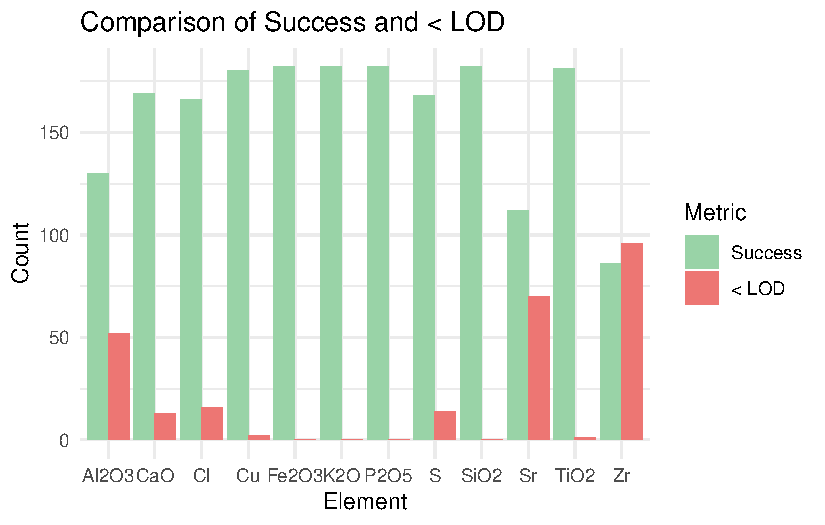
\includegraphics{geochemistry_files/figure-pdf/fig-lod-1.pdf}

}

\caption{\label{fig-lod-1}A barplot.}

\end{figure}%

\begin{figure}

\centering{

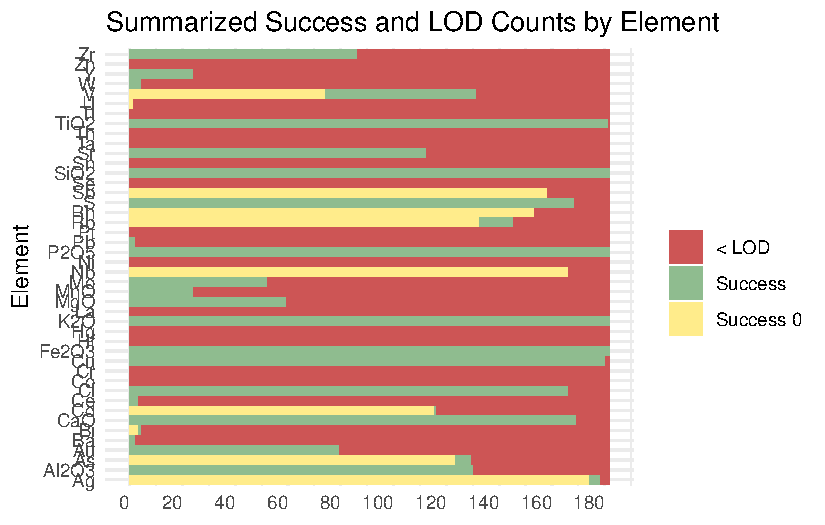
\includegraphics{geochemistry_files/figure-pdf/fig-lod-2.pdf}

}

\caption{\label{fig-lod-2}A barplot.}

\end{figure}%

\begin{verbatim}

Call:
PCA(X = df_scaled_alg, graph = FALSE) 


Eigenvalues
                       Dim.1   Dim.2   Dim.3   Dim.4   Dim.5   Dim.6   Dim.7
Variance               2.419   1.842   1.009   0.800   0.663   0.151   0.116
% of var.             34.558  26.319  14.408  11.424   9.477   2.154   1.660
Cumulative % of var.  34.558  60.877  75.284  86.708  96.186  98.340 100.000

Individuals (the 10 first)
          Dist    Dim.1    ctr   cos2    Dim.2    ctr   cos2    Dim.3    ctr
LJW   |  5.517 |  2.737  4.995  0.246 | -1.311  1.504  0.056 |  2.627 11.035
LJW.1 |  3.781 |  3.129  6.527  0.685 | -1.509  1.995  0.159 | -0.957  1.465
LJW.2 |  5.036 |  2.464  4.047  0.239 |  2.696  6.365  0.287 |  2.566 10.531
LJW.3 |  1.616 |  0.869  0.503  0.289 | -1.289  1.455  0.636 | -0.092  0.013
LJW.4 |  6.734 |  3.205  6.849  0.227 |  4.295 16.149  0.407 |  3.622 20.978
LJW.5 |  3.092 | -2.104  2.952  0.463 |  2.084  3.804  0.455 | -0.332  0.176
LJW.6 |  2.173 |  1.088  0.789  0.251 | -1.751  2.683  0.649 | -0.387  0.240
LJW.7 |  1.942 |  1.247  1.036  0.412 | -1.282  1.440  0.436 | -0.305  0.148
LJW.8 |  3.021 |  2.064  2.840  0.467 | -1.639  2.352  0.294 | -0.995  1.582
LJW.9 |  6.299 |  4.211 11.824  0.447 |  3.056  8.174  0.235 | -1.359  2.953
        cos2  
LJW    0.227 |
LJW.1  0.064 |
LJW.2  0.260 |
LJW.3  0.003 |
LJW.4  0.289 |
LJW.5  0.012 |
LJW.6  0.032 |
LJW.7  0.025 |
LJW.8  0.108 |
LJW.9  0.047 |

Variables
         Dim.1    ctr   cos2    Dim.2    ctr   cos2    Dim.3    ctr   cos2  
P2O5  |  0.805 26.793  0.648 |  0.490 13.038  0.240 | -0.148  2.184  0.022 |
S     |  0.659 17.966  0.435 |  0.491 13.067  0.241 | -0.154  2.358  0.024 |
Cl    |  0.360  5.358  0.130 |  0.474 12.190  0.225 |  0.611 37.034  0.374 |
K2O   |  0.667 18.400  0.445 | -0.675 24.757  0.456 | -0.141  1.971  0.020 |
CaO   |  0.081  0.270  0.007 |  0.596 19.287  0.355 | -0.379 14.249  0.144 |
TiO2  |  0.730 22.056  0.534 | -0.530 15.270  0.281 | -0.223  4.925  0.050 |
Fe2O3 |  0.471  9.157  0.222 | -0.210  2.391  0.044 |  0.613 37.279  0.376 |
\end{verbatim}

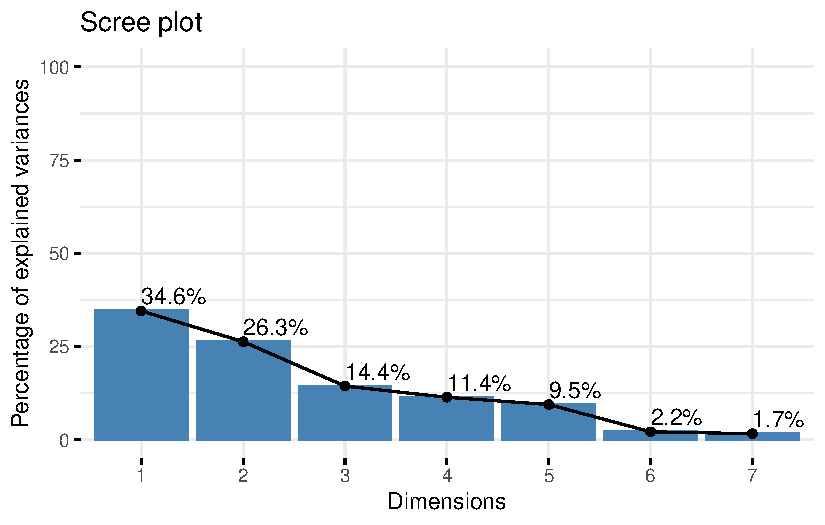
\includegraphics{geochemistry_files/figure-pdf/PCA-1.pdf}

\begin{verbatim}

Call:
PCA(X = df_scaled_nl, graph = FALSE) 


Eigenvalues
                       Dim.1   Dim.2   Dim.3   Dim.4   Dim.5   Dim.6
Variance               2.933   1.713   0.672   0.354   0.249   0.079
% of var.             48.885  28.546  11.197   5.901   4.157   1.314
Cumulative % of var.  48.885  77.431  88.628  94.529  98.686 100.000

Individuals (the 10 first)
          Dist    Dim.1    ctr   cos2    Dim.2    ctr   cos2    Dim.3    ctr
CPT   |  1.744 | -1.714  1.411  0.967 | -0.066  0.004  0.001 | -0.142  0.042
CPT.1 |  1.797 | -1.356  0.884  0.570 |  0.402  0.133  0.050 |  1.046  2.295
CPT.2 |  1.426 | -1.330  0.850  0.870 | -0.353  0.103  0.061 | -0.060  0.008
CPT.3 |  1.825 | -1.803  1.561  0.975 | -0.070  0.004  0.001 | -0.084  0.015
CPT.4 |  1.815 | -1.703  1.393  0.881 | -0.332  0.090  0.033 | -0.360  0.272
CPT.5 |  1.224 | -0.702  0.237  0.329 | -0.651  0.348  0.282 | -0.659  0.911
CPT.6 |  1.542 | -1.503  1.085  0.951 | -0.100  0.008  0.004 | -0.197  0.081
CPT.7 |  1.883 | -1.787  1.534  0.901 | -0.216  0.038  0.013 | -0.432  0.391
CPT.8 |  1.592 | -1.544  1.145  0.941 |  0.056  0.003  0.001 |  0.099  0.020
CPT.9 |  1.712 | -1.523  1.114  0.792 |  0.441  0.160  0.066 |  0.475  0.474
        cos2  
CPT    0.007 |
CPT.1  0.339 |
CPT.2  0.002 |
CPT.3  0.002 |
CPT.4  0.039 |
CPT.5  0.290 |
CPT.6  0.016 |
CPT.7  0.053 |
CPT.8  0.004 |
CPT.9  0.077 |

Variables
         Dim.1    ctr   cos2    Dim.2    ctr   cos2    Dim.3    ctr   cos2  
P2O5  |  0.668 15.194  0.446 |  0.591 20.375  0.349 | -0.119  2.094  0.014 |
K2O   |  0.836 23.802  0.698 | -0.463 12.504  0.214 | -0.073  0.791  0.005 |
TiO2  |  0.886 26.789  0.786 | -0.370  7.986  0.137 | -0.053  0.411  0.003 |
Fe2O3 |  0.844 24.304  0.713 | -0.237  3.278  0.056 |  0.110  1.797  0.012 |
Cu    |  0.411  5.761  0.169 |  0.632 23.299  0.399 |  0.637 60.406  0.406 |
S     |  0.349  4.150  0.122 |  0.747 32.557  0.558 | -0.481 34.501  0.232 |
\end{verbatim}

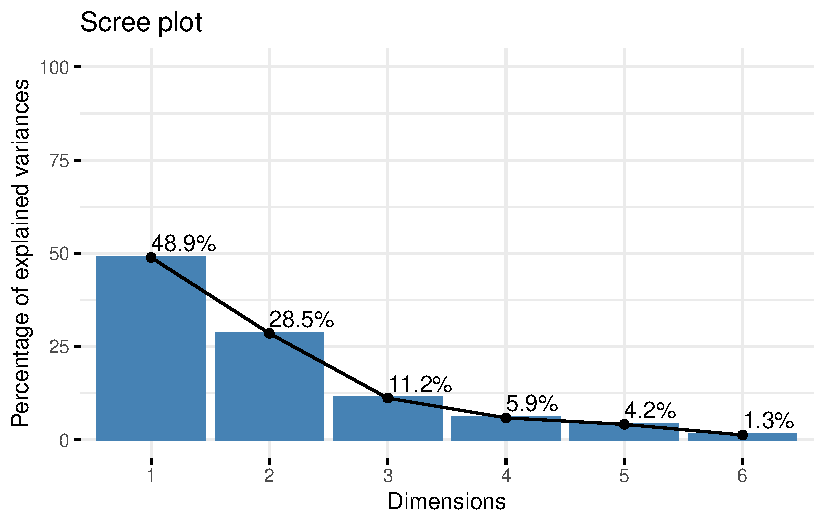
\includegraphics{geochemistry_files/figure-pdf/PCA-2.pdf}

\begin{verbatim}

Call:
PCA(X = df_scaled_comp, graph = FALSE) 


Eigenvalues
                       Dim.1   Dim.2   Dim.3   Dim.4   Dim.5   Dim.6
Variance               2.729   1.753   0.712   0.456   0.247   0.103
% of var.             45.477  29.222  11.871   7.600   4.121   1.709
Cumulative % of var.  45.477  74.699  86.570  94.170  98.291 100.000

Individuals (the 10 first)
          Dist    Dim.1    ctr   cos2    Dim.2    ctr   cos2    Dim.3    ctr
CPT   |  1.872 | -1.795  1.639  0.919 |  0.369  0.108  0.039 | -0.111  0.024
CPT.1 |  1.907 | -1.389  0.982  0.531 |  0.687  0.374  0.130 |  0.936  1.710
CPT.2 |  1.356 | -1.275  0.827  0.884 | -0.107  0.009  0.006 |  0.041  0.003
CPT.3 |  2.000 | -1.935  1.907  0.936 |  0.426  0.144  0.045 | -0.116  0.026
CPT.4 |  1.850 | -1.773  1.600  0.918 |  0.089  0.006  0.002 | -0.328  0.209
CPT.5 |  1.308 | -0.359  0.066  0.075 | -0.852  0.574  0.424 | -0.776  1.174
CPT.6 |  1.570 | -1.502  1.149  0.915 |  0.237  0.045  0.023 | -0.150  0.044
CPT.7 |  1.991 | -1.882  1.802  0.894 |  0.248  0.049  0.016 | -0.399  0.310
CPT.8 |  1.674 | -1.552  1.225  0.860 |  0.353  0.099  0.044 |  0.044  0.004
CPT.9 |  1.986 | -1.618  1.333  0.664 |  0.979  0.759  0.243 |  0.475  0.440
        cos2  
CPT    0.003 |
CPT.1  0.241 |
CPT.2  0.001 |
CPT.3  0.003 |
CPT.4  0.031 |
CPT.5  0.352 |
CPT.6  0.009 |
CPT.7  0.040 |
CPT.8  0.001 |
CPT.9  0.057 |

Variables
         Dim.1    ctr   cos2    Dim.2    ctr   cos2    Dim.3    ctr   cos2  
P2O5  |  0.663 16.108  0.440 |  0.620 21.955  0.385 | -0.190  5.080  0.036 |
K2O   |  0.712 18.598  0.507 | -0.630 22.626  0.397 | -0.108  1.653  0.012 |
TiO2  |  0.800 23.482  0.641 | -0.491 13.763  0.241 | -0.048  0.321  0.002 |
Fe2O3 |  0.751 20.672  0.564 | -0.247  3.491  0.061 |  0.295 12.221  0.087 |
Cu    |  0.463  7.866  0.215 |  0.576 18.943  0.332 |  0.617 53.383  0.380 |
S     |  0.602 13.273  0.362 |  0.581 19.222  0.337 | -0.441 27.342  0.195 |
\end{verbatim}

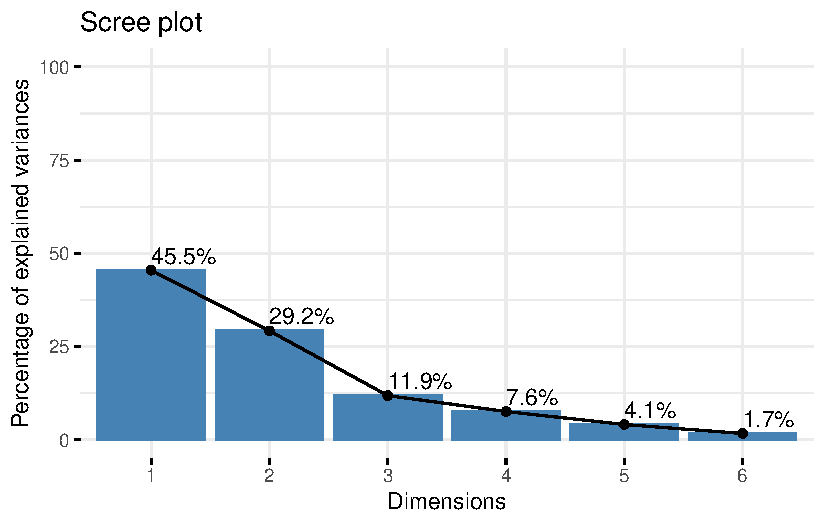
\includegraphics{geochemistry_files/figure-pdf/PCA-3.pdf}

\begin{verbatim}

Call:
PCA(X = df_scaled_comp2, graph = FALSE) 


Eigenvalues
                       Dim.1   Dim.2   Dim.3   Dim.4   Dim.5   Dim.6
Variance               3.074   1.638   0.687   0.329   0.237   0.035
% of var.             51.229  27.306  11.444   5.478   3.956   0.588
Cumulative % of var.  51.229  78.534  89.978  95.456  99.412 100.000

Individuals (the 10 first)
          Dist    Dim.1    ctr   cos2    Dim.2    ctr   cos2    Dim.3    ctr
LJW   |  3.502 |  1.688  0.997  0.232 | -0.419  0.115  0.014 |  0.306  0.147
LJW.1 |  1.452 |  1.128  0.445  0.604 |  0.594  0.232  0.168 | -0.644  0.649
LJW.2 |  2.521 |  0.866  0.262  0.118 |  1.892  2.350  0.563 | -1.389  3.020
LJW.3 |  0.560 |  0.044  0.001  0.006 | -0.390  0.100  0.485 | -0.313  0.153
LJW.4 |  3.148 |  1.069  0.400  0.115 |  2.767  5.026  0.773 | -0.431  0.290
LJW.5 |  1.545 | -1.026  0.368  0.441 |  0.339  0.076  0.048 | -1.094  1.876
LJW.6 |  0.899 |  0.196  0.013  0.048 | -0.082  0.004  0.008 | -0.832  1.084
LJW.7 |  1.453 | -0.219  0.017  0.023 | -0.853  0.478  0.345 |  0.961  1.445
LJW.8 |  0.819 |  0.167  0.010  0.041 | -0.546  0.196  0.445 |  0.524  0.430
LJW.9 |  6.112 |  1.021  0.365  0.028 |  4.521 13.412  0.547 |  3.411 18.220
        cos2  
LJW    0.008 |
LJW.1  0.197 |
LJW.2  0.303 |
LJW.3  0.313 |
LJW.4  0.019 |
LJW.5  0.502 |
LJW.6  0.857 |
LJW.7  0.437 |
LJW.8  0.410 |
LJW.9  0.311 |

Variables
         Dim.1    ctr   cos2    Dim.2    ctr   cos2    Dim.3    ctr   cos2  
P2O5  |  0.646 13.594  0.418 |  0.600 21.968  0.360 |  0.160  3.721  0.026 |
TiO2  |  0.921 27.594  0.848 | -0.316  6.092  0.100 |  0.052  0.399  0.003 |
K2O   |  0.889 25.723  0.791 | -0.371  8.410  0.138 |  0.114  1.903  0.013 |
Fe2O3 |  0.886 25.565  0.786 | -0.180  1.986  0.033 | -0.015  0.035  0.000 |
Cu    |  0.449  6.564  0.202 |  0.555 18.818  0.308 | -0.690 69.388  0.476 |
S     |  0.172  0.960  0.029 |  0.837 42.727  0.700 |  0.411 24.554  0.169 |
\end{verbatim}

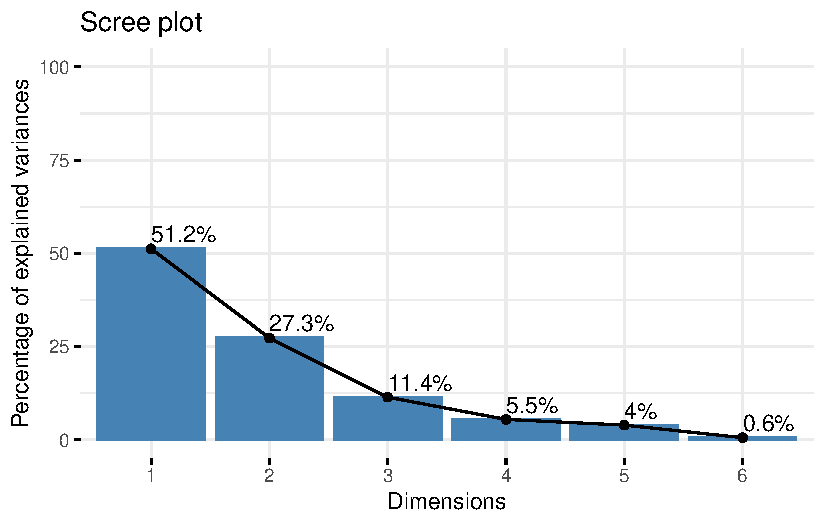
\includegraphics{geochemistry_files/figure-pdf/PCA-4.pdf}

\begin{figure}

\centering{

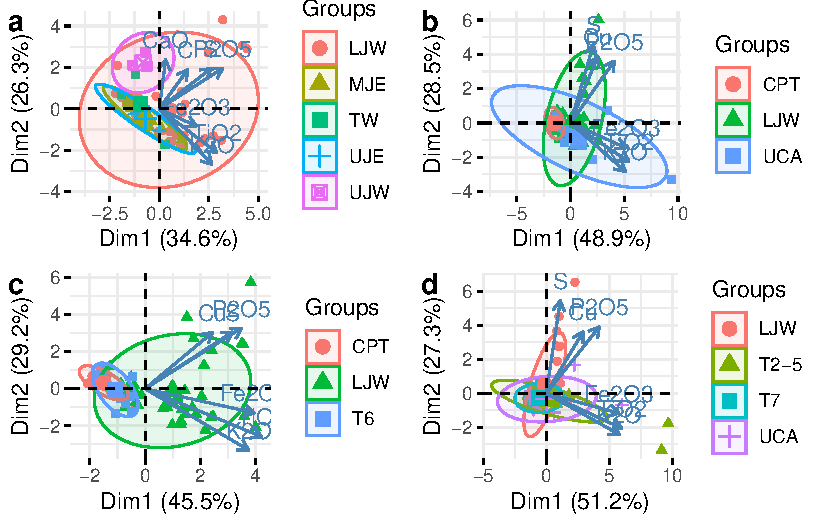
\includegraphics{geochemistry_files/figure-pdf/fig-pca-1.pdf}

}

\caption{\label{fig-pca}Several pcas}

\end{figure}%

\section{Methodology}\label{methodology}

For this experiment, a Bruker portable XRF Titan S1 was used in a
laboratory benchtop setup, using battery power (up to 25\% battery
charge then replaced by a fully charged battery). A validation run was
applied on two standard samples provided by Bruker and using the
standard calibration. Samples were scanned for 180 seconds each (90
seconds for the first phase for major elements and 90 seconds for the
second phase for minor elements), at least once, with several scans
applied to samples that showed macroscopic variability (e.g., areas with
different colours or translucency). The standard database from Bruker
was used, with the Geochem application and Dual Mining method. ** chert
samples were scanned, from several sources and chert types, both
geological and archaeological. After scanning, the scanned face was
measured (thickness and diameter), to guarantee a minimum thickness and
size was followed for each sample, since other studies have shown
thickness and size may impact the homogeneity of data collection and
results (Newlander et al. 2015). All samples, including their thickness
and diameter, can be found in table X. For geological samples, fresh,
flat surfaces were scanned, avoiding altered faces or cortex; whenever
necessary, the samples were prepared by breaking the nodules. The
samples were chosen to represent all varieties of chert identified in
the Algarve region, in the archaeological record of Vale Boi, but also
from other regions such as Central Portugal and South Spain, to allow
their comparison and test hypotheses made from macroscopic and
petrographic data. For archaeological samples, artefacts were chosen
from previously identified types (REF?), focusing on larger and flatter
morphologies, with the least degree of surface alterations possible.

The analysis and result reporting protocol was established following
previous studies, focusing on the accuracy of obtained data but also the
transparency and reproducibility of the results (Newlander et al. 2015;
Johnson et al. 2024). For further reproducibility and replicability, and
working towards the goal of open science (Johnson et al. 2024; Marwick
2017), the obtained raw pXRF results can be found online on our online
compendium (LINK).

\section{Results}\label{results-2}

The pXRF measured several major and minor elements, of which a small
amount returned values of 0 or were below the limit of detection
(\textless LOD). These were uranium (U), thorium (Th), bismuth (Bi),
thallium (Tl), mercury (Hg), platinum (Pt), tantalum (Ta), hafnium (Hf),
lanthanum (La), antimony (Sb), Tin (Sn), cadmium (Cd), rhodium (Rh),
niobium (Nb), selenium (Se), zinc (Zn), nickel (Ni), cobalt (Co) and
chromium (Cr). They were removed from the analysis based on their
nonexistence, although they can still be found in the raw pXRF results.

\bookmarksetup{startatroot}

\chapter{From Stone to Tool}\label{from-stone-to-tool}

\bookmarksetup{startatroot}

\chapter{Discussion and final
remarks}\label{discussion-and-final-remarks}

\bookmarksetup{startatroot}

\chapter*{References}\label{references}
\addcontentsline{toc}{chapter}{References}

\markboth{References}{References}

\phantomsection\label{refs}
\begin{CSLReferences}{1}{0}
\bibitem[\citeproctext]{ref-abrunhosaUseDigitalMobile2017}
Abrunhosa, Ana, J. Cascalheira, Alfredo Pérez-González, Juan Arsuaga,
and Enrique Baquedano. 2017. {``The Use of Digital Mobile Technologies
for Geoarchaeological Survey: {The} Example of the {Pinilla} Del {Valle}
Raw Material Project.''} In \emph{Proceedings of the 12th {International
Conference} of {Archaeological Prospection}}, 3--4. Archaeopress.

\bibitem[\citeproctext]{ref-ambroseSocialEcologicalModels1990}
Ambrose, S, and K Lorenz. 1990. {``Social and Ecological Models for the
Middle Stone Age in Southern {Africa}.''} In \emph{The Emergence of
Modern Humans: An Archaeological Perspective}, 3--33. Edinburgh:
Edinburgh University Press.

\bibitem[\citeproctext]{ref-aubryFarFlintInferring2022}
Aubry, Thierry, António Fernando Barbosa, Cristina Gameiro, Luís Luís,
André Tomás Santos, and Marcelo Silvestre. 2022. {``Far from Flint:
{Inferring} Land-Use and Social Networks from {Middle} and {Upper
Palaeolithic} Lithic Assemblages ({Cardina-Salto} Do {Boi}, {C{ô}a
Valley}, {Portugal}).''} \emph{Journal of Archaeological Science:
Reports} 42. \url{https://doi.org/10.1016/j.jasrep.2022.103385}.

\bibitem[\citeproctext]{ref-aubryUpperPalaeolithicLithic2016}
Aubry, Thierry, Cristina Gameiro, Javier Mangado Llach, Luís Luís,
Henrique Matias, and Tiago Do Pereiro. 2016. {``Upper {Palaeolithic}
Lithic Raw Material Sourcing in {Central} and {Northern Portugal} as an
Aid to Reconstructing Hunter-Gatherer Societies.''} \emph{Journal of
Lithic Studies} 3 (2): 7--28.
\url{https://doi.org/10.2218/jls.v3i2.1436}.

\bibitem[\citeproctext]{ref-aubryEconomyLithicRaw2009}
Aubry, Thierry, and M de Araújo Igreja. 2009. {``Economy of Lithic Raw
Material During the {Upper Paleolithic} of the {C{ô}a Valley} and the
{Sic{ó} Massif} ({Portugal}): Technological and Functional
Perspectives.''} In \emph{Proceedings of the {Workshop Functional
Studies} of {Non Flint Stone Tools}: {Methodological Improvements} and
{Archaeological Inferences}}, 26. Lisbon.

\bibitem[\citeproctext]{ref-aubryRawMaterialProcurement2004}
Aubry, Thierry, X Mangado, J Fullola, L Rosell, and J Sampaio. 2004.
{``The Raw Material Procurement at the {Upper Palaeolithic} Settlements
of the {C{ô}a Valley} ({Portugal}): New Data Concerning Modes of
Resource Exploitation in {Iberia}.''} In \emph{The {Use} of {Living
Space} in {Prehistory}: {Papers} from a Session Held at the {European
Association} of {Archaeologists Sixth Annual Meeting} in {Lisbon} 2000},
37--50. Oxford: Archeopress (BAR International Series; 1224).

\bibitem[\citeproctext]{ref-bamforth_technology_1997}
Bamforth, Douglas B., and Peter Bleed. 1997. {``Technology, {Flaked
Stone Technology}, and {Risk}.''} \emph{Archaeological Papers of the
American Anthropological Association} 7 (1): 109--39.
\url{https://doi.org/10.1525/ap3a.1997.7.1.109}.

\bibitem[\citeproctext]{ref-banksHumanEcologicalNiches2008}
Banks, William, Francesco d'Errico, Andrew Peterson, Marian Vanhaeren,
Masa Kageyama, Pierre Sepulchre, Gilles Ramstein, Anne Jost, and Dale
Lunt. 2008. {``Human Ecological Niches and Ranges During the {LGM} in
{Europe} Derived from an Application of Eco-Cultural Niche Modeling.''}
\emph{Journal of Archaeological Science} 35 (February): 481--91.
\url{https://doi.org/10.1016/j.jas.2007.05.011}.

\bibitem[\citeproctext]{ref-bar-yosef2002}
Bar-Yosef, Ofer. 2002. {``The Upper Paleolithic Revolution.''}
\emph{Annual Review of Anthropology} 31 (Volume 31, 2002): 363--93.
\url{https://doi.org/10.1146/annurev.anthro.31.040402.085416}.

\bibitem[\citeproctext]{ref-belmiroProtoSolutreanLithicTechnology2020}
Belmiro, Joana. 2020. {``Proto-{Solutrean} Lithic Technology of Western
{Iberia}: The Sites of {Vale Boi} and {Lapa} Do {Picareiro}.''} Master's
thesis.

\bibitem[\citeproctext]{ref-belmiro_gravettian-solutrean_2021}
Belmiro, Joana, Nuno Bicho, Jonathan Haws, and João Cascalheira. 2021.
{``The {Gravettian-Solutrean} Transition in Westernmost {Iberia}: {New}
Data from the Sites of {Vale Boi} and {Lapa} Do {Picareiro}.''}
\emph{Quaternary International}, The 3rd {Conference World} of
{Gravettian Hunters}, 587--588 (June): 19--40.
\url{https://doi.org/10.1016/j.quaint.2020.08.027}.

\bibitem[\citeproctext]{ref-belmiroCreatingFramesReference2023}
Belmiro, Joana, Xavier Terradas, and João Cascalheira. 2023. {``Creating
Frames of Reference for Chert Exploitation During the {Late Pleistocene}
in {Southwesternmost Iberia}.''} \emph{PLOS ONE} 18 (10): e0293223.
\url{https://doi.org/10.1371/journal.pone.0293223}.

\bibitem[\citeproctext]{ref-belmiroChertProcurementPatterns2025}
Belmiro, Joana, Xavier Terradas, Salvador Dominguez-Bella, and João
Cascalheira. 2025. {``Within and {Beyond}: {Chert Procurement Patterns
During The Upper Palaeolithic} in {Southwesternmost Iberia}.''}
\emph{Journal of Paleolithic Archaeology} 8 (1): 8.
\url{https://doi.org/10.1007/s41982-025-00209-2}.

\bibitem[\citeproctext]{ref-bicho_at_2008}
Bicho, N, and J Haws. 2008. {``At the Land's End: {Marine} Resources and
the Importance of Fluctuations in the Coastline in the Prehistoric
Hunter--Gatherer Economy of {Portugal}.''} \emph{Quaternary Science
Reviews} 27 (23-24): 2166--75.
\url{https://doi.org/10.1016/j.quascirev.2008.08.011}.

\bibitem[\citeproctext]{ref-bichoEdgeCaseVale2012}
Bicho, Nuno, J. Cascalheira, and Joao Marreiros. 2012. {``On the
({L})edge:: {The Case} of {Vale Boi Rockshelter} ({Algarve}, {Southern
Portugal}).''} In \emph{Caves in {Context}. {The Cultural Significance}
of {Caves} and {Rockshelters} in {Europe}}, 65--81. Oxford: Oxbow Books.
\url{https://doi.org/10.2307/j.ctvh1djk4.10}.

\bibitem[\citeproctext]{ref-bichoEarlyUpperPaleolithic2017}
Bicho, Nuno, João Cascalheira, and Célia Gonçalves. 2017. {``Early
{Upper Paleolithic} Colonization Across {Europe}: {Time} and Mode of the
{Gravettian} Diffusion.''} \emph{PLOS ONE} 12 (5): e0178506.
\url{https://doi.org/10.1371/journal.pone.0178506}.

\bibitem[\citeproctext]{ref-bicho_rapid_2017-1}
Bicho, Nuno, João Cascalheira, João Marreiros, and Telmo Pereira. 2017b.
{``Rapid Climatic Events and Long Term Cultural Change: {The} Case of
the {Portuguese Upper Paleolithic}.''} \emph{Quaternary International}
428: 3--16. \url{https://doi.org/10.1016/j.quaint.2015.05.044}.

\bibitem[\citeproctext]{ref-bicho2017}
---------. 2017a. {``Rapid Climatic Events and Long Term Cultural
Change: The Case of the Portuguese Upper Paleolithic.''}
\emph{Quaternary International} 428: 3--16.
\url{https://doi.org/10.1016/j.quaint.2015.05.044}.

\bibitem[\citeproctext]{ref-bichoPleistoceneHuntergathererCoastal2022}
Bicho, Nuno, and Eduardo Esteves. 2022. {``Pleistocene Hunter-Gatherer
Coastal Adaptations in {Atlantic Iberia}.''} \emph{Frontiers in Earth
Science} 10 (August). \url{https://doi.org/10.3389/feart.2022.957214}.

\bibitem[\citeproctext]{ref-bicho2012}
Bicho, Nuno, and Jonathan Haws. 2012. {``The Magdalenian in Central and
Southern Portugal: Human Ecology at the End of the Pleistocene.''}
\emph{Quaternary International} 272-273 (September): 6--16.
\url{https://doi.org/10.1016/j.quaint.2012.02.055}.

\bibitem[\citeproctext]{ref-bicho_ecodynamics_2013}
Bicho, Nuno, Tiina Manne, João Marreiros, João Cascalheira, Telmo
Pereira, Frederico Tátá, Marina Évora, Célia Gonçalves, and Leandro
Infantini. 2013. {``The Ecodynamics of the First Modern Humans in
{Southwestern Iberia}: {The} Case of {Vale Boi}, {Portugal}.''}
\emph{Quaternary International} 318: 102--16.
\url{https://doi.org/10.1016/j.quaint.2013.06.029}.

\bibitem[\citeproctext]{ref-bicho_o_2003}
Bicho, Nuno, Mary Stiner, John Lindly, and C. Reid Ferring. 2003. {``O
{Mesol{í}tico} e o {Neol{í}tico} Antigo Da Costa Algarvia.''} In
\emph{Muita Gente Poucas Antas? {Origens}, Espa{ç}os e Contextos Do
{Megalitismo}.}, 15--22. Lisboa: Instituto Portugu{ê}s de Arqueologia.

\bibitem[\citeproctext]{ref-bichoRockshelterStudiesSouthwestern2007}
Bicho, Nuno, Mary Stiner, Delminda Moura, and Armando Lucena. 2007.
{``Rockshelter Studies in Southwestern {Iberia}: The Case of Vale Boi
({Algarve}, Southern Portugal).''} In \emph{On {Shelter}'s {Ledge}:
{Histories Theories} and {Methods} of {Rockshelter Research} /{Pr{é}s}
Du Bord d'un Abri: {Les} Histories Th{é}ories Et m{é}thodes de
Recherches}, 75--82. {BAR International Series} 1655. BAR Publishing,
Oxford.

\bibitem[\citeproctext]{ref-binfordOrganizationFormationProcesses1979}
Binford, Lewis R. 1979. {``Organization and {Formation Processes}:
{Looking} at {Curated Technologies} {\textbar} {Journal} of
{Anthropological Research}: {Vol} 35, {No} 3.''} \emph{Journal of
Anthropological Research} 35 (3).
\url{https://doi.org/10.1086/jar.35.3.3629902}.

\bibitem[\citeproctext]{ref-binford_righteous_1985}
Binford, Lewis R., and Nancy M. Stone. 1985. {``{`{Righteous Rocks}'}
and {Richard Gould}: {Some Observations} on {Misguided} {`{Debate}'}.''}
\emph{American Antiquity} 50 (1): 151--53.
\url{https://doi.org/10.2307/280641}.

\bibitem[\citeproctext]{ref-bleedOptimalDesignHunting1986}
Bleed, Peter. 1986. {``The {Optimal Design} of {Hunting Weapons}:
{Maintainability} or {Reliability}.''} \emph{American Antiquity} 51 (4):
737--47. \url{https://doi.org/10.2307/280862}.

\bibitem[\citeproctext]{ref-boessenkoolNorthAtlanticSeasurface2001}
Boessenkool, Karin, Henk Brinkhuis, Joachim Schönfeld, and Jordi
Targarona. 2001. {``North Atlantic Sea-Surface Temperature Changes and
the Climate of Western Iberia During the Last Deglaciation; a Marine
Palynological Approach.''} \emph{Global and Planetary Change} 30
(September). \url{https://doi.org/10.1016/S0921-8181(01)00075-3}.

\bibitem[\citeproctext]{ref-boudagher-fadelChapterMesozoicLarger2008}
BouDagher-Fadel, Marcelle K. 2008. {``Chapter 4 {The Mesozoic} Larger
Benthic Foraminifera: The {Jurassic}.''} In \emph{Developments in
{Palaeontology} and {Stratigraphy}}, 21:157--542. Elsevier.
\url{https://doi.org/10.1016/S0920-5446(08)00004-6}.

\bibitem[\citeproctext]{ref-bousmanHuntergathererAdaptationsEconomic1993}
Bousman, Britt. 1993. {``Hunter-Gatherer Adaptations, Economic Risk and
Tool Design.''} \emph{Lithic Technology} 18 (1/2): 59--86.

\bibitem[\citeproctext]{ref-bradtmoller_lithic_2016}
Bradtmöller, Marcel, João Marreiros, Telmo Pereira, and Nuno Bicho.
2016. {``Lithic Technological Adaptation Within the {Gravettian} of the
{Iberian Atlantic} Region: {Results} from Two Case Studies.''}
\emph{Quaternary International} 406: 3--24.
\url{https://doi.org/10.1016/j.quaint.2015.08.075}.

\bibitem[\citeproctext]{ref-bradtmoller_repeated_2012-1}
Bradtmöller, Marcel, Andreas Pastoors, Bernhard Weninger, and
Gerd-Christian Weniger. 2012. {``The Repeated Replacement Model --
{Rapid} Climate Change and Population Dynamics in {Late Pleistocene
Europe}.''} \emph{Quaternary International} 247: 38--49.
\url{https://doi.org/10.1016/j.quaint.2010.10.015}.

\bibitem[\citeproctext]{ref-brantinghamNeutralModelStone2003}
Brantingham, P. 2003. {``A {Neutral Model} of {Stone Raw Material
Procurement}.''} \emph{American Antiquity} 68 (July).
\url{https://doi.org/10.2307/3557105}.

\bibitem[\citeproctext]{ref-brantinghamMeasuringForagerMobility2006}
Brantingham, P. Jeffrey. 2006. {``Measuring {Forager Mobility}.''}
\emph{Current Anthropology} 47 (3): 435--59.
\url{https://doi.org/10.1086/503062}.

\bibitem[\citeproctext]{ref-bressyCaracterisationGestionSilex2002}
Bressy, Céline. 2002. {``Caracterisation Et Gestion Du Silex Des Sites
Mesolithiques Et Neolithiques Du {Nord-Ouest} de {L}'{Arc Alpin}. {Une}
Approche p{é}trographique Et g{é}ochimique.''} Doctoral Thesis, France:
Universit{é} de Aix-Marseille.

\bibitem[\citeproctext]{ref-brown_raw_1999}
Brown, Kimberly. 1999. \emph{Raw Material Selection and Flake Production
in the {Middle Stone Age} of {Southern Africa}: {Die Kelders Cave I} and
{Montagu Cave}.} State University of New York at Stony Brook.

\bibitem[\citeproctext]{ref-bustilloMacroscopicClassificationFlint2009}
Bustillo, M. A., N. Castañeda, M. Capote, S. Consuegra, C. Criado, P.
Díaz-Del-Río, T. Orozco, J. L. Pérez-Jiménez, and X. Terradas. 2009.
{``Is the Macroscopic Classification of Flint Useful? {A}
Petroarcharological Analysis and Characterization of Flint Raw Materials
from the {Iberian} Neolithic Mine of {Casa Montero}.''}
\emph{Archaeometry} 51 (2): 175--96.
\url{https://doi.org/10.1111/j.1475-4754.2008.00403.x}.

\bibitem[\citeproctext]{ref-cardosoSobrePresencaLaminas2018}
Cardoso, João Luís, Marco António Andrade, and Filipe Martins. 2018.
{``{Sobre a presen{ç}a de l{â}minas de s{í}lex Ool{í}tico (e outras
mat{é}rias-primas ex{ó}genas) no povoado Calcol{í}tico do
Outeiro~Redondo (Sesimbra, Portugal): interac{ç}{ã}o durante o
3.º mil{é}nio a.C. no Sudoeste Peninsular}.''} \emph{Estudos
Arqueol{ó}gicos de Oeiras} 24: 61.

\bibitem[\citeproctext]{ref-carvalho_neanderthal_2022}
Carvalho, Milena, Emily Lena Jones, M. Grace Ellis, João Cascalheira,
Nuno Bicho, David Meiggs, Michael Benedetti, Lukas Friedl, and Jonathan
Haws. 2022. {``Neanderthal Palaeoecology in the Late {Middle
Palaeolithic} of Western {Iberia}: A Stable Isotope Analysis of Ungulate
Teeth from {Lapa} Do {Picareiro} ({Portugal}).''} \emph{Journal of
Quaternary Science} 37 (2): 300--319.
\url{https://doi.org/10.1002/jqs.3363}.

\bibitem[\citeproctext]{ref-cascalheiraTecnologiaLiticaSolutrense2010}
Cascalheira, João. 2010. \emph{{Tecnologia L{í}tica Solutrense do Abrigo
de Vale Boi (Vila do Bispo)}}. {Cadernos da UNIARQ} 5. UNIARQ.

\bibitem[\citeproctext]{ref-cascalheiraSolutrenseEmPortugal2013}
---------. 2013. {``{O solutrense em portugal: novidades do s{é}culo
xxi}.''}

\bibitem[\citeproctext]{ref-cascalheiraTerritorialityOrganizationTechnology2019}
---------. 2019. {``Territoriality and the Organization of Technology
During the {Last Glacial Maximum} in Southwestern {Europe}.''}
\emph{PLOS ONE} 14 (12): e0225828.
\url{https://doi.org/10.1371/journal.pone.0225828}.

\bibitem[\citeproctext]{ref-cascalheiraHunterGathererEcodynamics2013}
Cascalheira, João, and Nuno Bicho. 2013. {``Hunter--Gatherer Ecodynamics
and the Impact of the {Heinrich} Event 2 in {Central} and {Southern
Portugal}.''} \emph{Quaternary International} 318 (December): 117--27.
\url{https://doi.org/10.1016/j.quaint.2013.05.039}.

\bibitem[\citeproctext]{ref-cascalheira_b_2017}
Cascalheira, João, Nuno Bicho, and Célia Gonçalves. 2017. {``A
{Google-Based Freeware Solution} for {Archaeological Field Survey} and
{Onsite Artifact Analysis}.''} \emph{Advances in Archaeological
Practice} 5 (4): 328--39. \url{https://doi.org/10.1017/aap.2017.21}.

\bibitem[\citeproctext]{ref-cascalheira_2017}
Cascalheira, João, Nuno Bicho, Tiina Manne, and Pedro Horta. 2017.
{``Cross-Scale Adaptive Behaviors During the {Upper Paleolithic} in
{Iberia}: {The} Example of {Vale Boi} ({Southwestern Portugal}).''}
\emph{Quaternary International}, Adaptive {Cycles} in {Archaeology}, 446
(August): 17--30. \url{https://doi.org/10.1016/j.quaint.2017.01.002}.

\bibitem[\citeproctext]{ref-cascalheiraValeBoiAlgarve2013}
Cascalheira, João, Nuno Bicho, João Marreiros, Telmo Pereira, Marina
Évora, Miguel Cortés, Juan Gibaja, et al. 2013. {``Vale {Boi}
({Algarve}, {Portugal}) and the {Solutrean} in {Southwestern Iberia}.''}
\emph{Espacio Tiempo y Forma. Serie I, Prehistoria y Arqueolog{í}a} 1
(5). \url{https://doi.org/10.5944/etfi.5.2012.5376}.

\bibitem[\citeproctext]{ref-consuegraMitochondrialDNAVariation2002}
Consuegra, S., C. García de Leániz, A. Serdio, M. González Morales, L.
G. Straus, D. Knox, and E. Verspoor. 2002. {``Mitochondrial {DNA}
Variation in {Pleistocene} and Modern {Atlantic} Salmon from the
{Iberian} Glacial Refugium.''} \emph{Molecular Ecology} 11 (10):
2037--48. \url{https://doi.org/10.1046/j.1365-294x.2002.01592.x}.

\bibitem[\citeproctext]{ref-corchonrodriguezMobiliteTerritoiresRelations2016}
Corchón Rodríguez, Soledad, Jimena Martínez, and Antonio Tarriño. 2016.
{``Mobilit{é}, Territoires Et Relations Culturelles Au d{é}but Du
{Magdal{é}nien} Moyen Cantabrique : Nouvelles Perspectives.''} In
\emph{Le Concept de Territoires Dans Le {Pal{é}olithique} Sup{é}rieur
Europ{é}en}. Vol. 3, Session C16. {BAR British Archaeological Reports
International}. Oxford: Bar Publishing.

\bibitem[\citeproctext]{ref-costaLithicArrowheadsSiliceous2022}
Costa, Mafalda, Luís Dias, Leonor Rocha, Jorge Oliveira, Pedro Barrulas,
and José Mirão. 2022. {``Lithic Arrowheads: {Siliceous} Raw Material
Sources and Technology in {Southern Portugal}.''} \emph{Geoarchaeology}
37 (3): 560--73. \url{https://doi.org/10.1002/gea.21891}.

\bibitem[\citeproctext]{ref-crandellMacroscopicAnalysisCharacterisation2005}
Crandell, Otis. 2005. {``Macroscopic {Analysis} and {Characterisation}
of {Chert} for {Provenance Purposes}.''} \emph{Sargetia, Acta Musei
Devensis} 33: 137--53.

\bibitem[\citeproctext]{ref-dalen_partial_2012}
Dalen, L., L. Orlando, B. Shapiro, M. Brandstrom-Durling, R. Quam, M. T.
P. Gilbert, J. C. Diez Fernandez-Lomana, E. Willerslev, J. L. Arsuaga,
and A. Gotherstrom. 2012. {``Partial {Genetic Turnover} in
{Neandertals}: {Continuity} in the {East} and {Population Replacement}
in the {West}.''} \emph{Molecular Biology and Evolution} 29 (8):
1893--97. \url{https://doi.org/10.1093/molbev/mss074}.

\bibitem[\citeproctext]{ref-delagnesExploitationSilexAu2006}
Delagnes, Anne, Jéhanne Féblot-Augustins, Liliane Meignen, and Seong-Jin
Park. 2006. {``{L'exploitation des silex au Pal{é}olithique moyen dans
le Bassin de la Charente: qu'est-ce qui circule, comment... et
pourquoi?}''} \emph{Bulletin de liaison et d'information de
l'Association des Arch{é}ologues de Poitou-Charentes} 35: 15--24.
\url{https://doi.org/halshs00447484}.

\bibitem[\citeproctext]{ref-delluniversitaDevelopmentMultiparametricCharacterisation2019}
Delluniversità, Emanuela, Italo Maria Muntoni, Ignazio Allegretta,
Massimo Tarantini, Alessandro Monno, Patrizia Maiorano, Angela Girone,
Michele Morsilli, Roberto Terzano, and Giacomo Eramo. 2019.
{``Development of a Multiparametric Characterisation Protocol for Chert
Investigation and Application on the {Gargano Promontory} Mines.''}
\emph{Archaeological and Anthropological Sciences} 11 (11): 6037--63.
\url{https://doi.org/10.1007/s12520-019-00875-8}.

\bibitem[\citeproctext]{ref-delvigneGeoresourcesTechnoculturalExpressions2019}
Delvigne, Vincent, Paul Fernandes, Peter Bindon, Jean-Pierre Bracco,
Laurent Klaric, Audrey Lafarge, Mathieu Langlais, Michel Piboule, and
Jean-Paul Raynal. 2019. {``Geo-Resources and Techno-Cultural Expressions
in the South of the {French Massif Central} During the {Upper
Palaeolithic}: Determinism and Choices.''} \emph{Anthropologica Et
Pr{æ}historica} 128/2017: 39--55.

\bibitem[\citeproctext]{ref-dias_coast_2000}
Dias, J M A, T Boski, A Rodrigues, and F MagalhaÄes. 2000. {``Coast Line
Evolution in {Portugal} Since the {Last Glacial Maximum} Until Present
{\DH} a Synthesis.''} \emph{Marine Geology}, 10.

\bibitem[\citeproctext]{ref-dias_evolucao_1997}
Dias, Joao, A. Rodrigues, and Fernando Magalhães. 1997. {``Evolu{ç}{ã}o
Da Linha de Costa, Em {Portugal}, Desde o {Ú}ltimo m{á}ximo Glaci{á}rio
at{é} {à} Actualidade: {S{í}ntese} Dos Conhecimentos.''} \emph{Estudos
Do Quatern{á}rio} 1: 53--66. \url{https://doi.org/10.30893/eq.v0i1.8}.

\bibitem[\citeproctext]{ref-diazdelrioWhatIberianCopper2020}
Díaz del Río, Pedro. 2020. {``What the {Iberian Copper Age} Can Tell Us
about Peasant Societies, and Vice Versa.''} In \emph{Archaeology and
History of Peasantries}, 41--54. Documentos de Arqueolog{í}a Medieval
14, 16. Bilbao: Universidad del Pa{í}s Vasco.

\bibitem[\citeproctext]{ref-dominguezbellaMineralesRocasSociedades2010}
Domínguez Bella, Salvador. 2010. \emph{{Minerales y rocas en las
sociedades de la Prehistoria}}. C{á}diz: Grupo de Investigaci{ó}n
HUM-440, Universidad de C{á}diz.

\bibitem[\citeproctext]{ref-dominguez-bellaEstudioMateriasPrimas2006}
Domínguez-Bella, Salvador. 2006. {``El Estudio de Las Materias Primas En
La {Prehistoria} Del {Á}mbito Gaditano.''} In \emph{Actas de {I Seminaro
Hispano-Marroqu{í}} de Especializaci{ó}n En Arqueolog{í}a}, 77--88.
Universidad de C{á}diz.

\bibitem[\citeproctext]{ref-driscollIntroducingLIRLithotheque2016}
Driscoll, Killian, Adrian L. Burke, and Graeme M. Warren. 2016.
{``Introducing {LIR} ({Lithotheque Ireland}), a Reference Collection of
Flaked Stone Tool Raw Materials from {Ireland}.''} \emph{Journal of
Lithic Studies} 3 (2): 231--51.
\url{https://doi.org/10.2218/jls.v3i2.1444}.

\bibitem[\citeproctext]{ref-ekshtainRawMaterialExploitation2022}
Ekshtain, Ravid, and Yossi Zaidner. 2022. {``Raw Material Exploitation
at the {Middle Paleolithic} Site of {Nesher Ramla}, {Israel}.''}
\emph{Quaternary International} 624: 34--48.
\url{https://doi.org/10.1016/j.quaint.2021.02.038}.

\bibitem[\citeproctext]{ref-feblot-augustinsMobilityStrategiesLate1993}
Féblot-Augustins, Jehanne. 1993. {``Mobility {Strategies} in the {Late
Middle Palaeolithic} of {Central Europe} and {Western Europe}:
{Elements} of {Stability} and {Variability}.''} \emph{Journal of
Anthropological Archaeology} 12 (3): 211--65.
\url{https://doi.org/10.1006/jaar.1993.1007}.

\bibitem[\citeproctext]{ref-fernandesNewEvidenceConcerning2012}
Fernandes, Paulo, Jennifer A. Musgrave, Geoff Clayton, Zélia Pereira,
José Tomás Oliveira, Robbie Goodhue, and Bruno Rodrigues. 2012. {``New
Evidence Concerning the Thermal History of {Devonian} and
{Carboniferous} Rocks in the {South Portuguese Zone}.''} \emph{Journal
of the Geological Society} 169 (6): 647--54.
\url{https://doi.org/10.1144/jgs2011-156}.

\bibitem[\citeproctext]{ref-fernandesMapDatabaseFlintbearing2013}
Fernandes, Paul, Jean-Paul Raynal, Pascal Tallet, Christophe Tuffery,
Michel Piboule, Micheline Séronie-Vivien, Marie-Roger Séronie-Vivien, et
al. 2013. {``A Map and a Database for Flint-Bearing Formations in
{Southern France}: {A} Tool for {Petroarchaeology}.''} \emph{Pal{é}o},
no. 24 (December): 219--28. \url{https://doi.org/10.4000/paleo.2864}.

\bibitem[\citeproctext]{ref-fernandesSilexBergeracoisEtat2012}
Fernandes, P, A Morala, P Schmidt, Marie-Roger Séronie-Vivien, and Alain
Turq. 2012. {``{Le silex du Bergeracois : {é}tat de la question}.''}
\emph{Quaternaire Continental d'Aquitaine, excursion AFEQ - ASF 2012},
22--44.

\bibitem[\citeproctext]{ref-finlayson_late_2006}
Finlayson, Clive, Francisco Giles Pacheco, Joaquín Rodríguez-Vidal,
Darren A. Fa, José María Gutierrez López, Antonio Santiago Pérez,
Geraldine Finlayson, et al. 2006. {``Late Survival of {Neanderthals} at
the Southernmost Extreme of {Europe}.''} \emph{Nature} 443 (7113):
850--53. \url{https://doi.org/10.1038/nature05195}.

\bibitem[\citeproctext]{ref-fletcherMillennialscaleVariabilityLast2010}
Fletcher, William J., Maria Fernanda Sánchez Goñi, Judy R. M. Allen,
Rachid Cheddadi, Nathalie Combourieu-Nebout, Brian Huntley, Ian Lawson,
et al. 2010. {``Millennial-Scale Variability During the Last Glacial in
Vegetation Records from {Europe}.''} \emph{Quaternary Science Reviews},
Vegetation {Response} to {Millennial-scale Variability} during the {Last
Glacial}, 29 (21): 2839--64.
\url{https://doi.org/10.1016/j.quascirev.2009.11.015}.

\bibitem[\citeproctext]{ref-fletcherOrbitalSuborbitalscaleClimate2008}
Fletcher, William, and Maria Sanchez Goñi. 2008. {``Orbital- and
Sub-Orbital-Scale Climate Impacts on Vegetation of the Western
{Mediterranean} Basin over the Last 48,000 Yr.''} \emph{Quaternary
Research} 70 (November): 451--64.
\url{https://doi.org/10.1016/j.yqres.2008.07.002}.

\bibitem[\citeproctext]{ref-flugelMicrofaciesCarbonateRocks2010}
Flügel, Erik. 2010. \emph{Microfacies of {Carbonate Rocks}}. Berlin,
Heidelberg: Springer. \url{https://doi.org/10.1007/978-3-642-03796-2}.

\bibitem[\citeproctext]{ref-forteaperezCuevaMallaetesProblemas1975}
Fortea Pérez, F. Javier, and Francisco Jordá Cerda. 1975. {``La Cueva de
Les Mallaetes y Los Problemas Del Paleolítico Superior Del Mediterráneo
Español.''} \emph{Zephyrvs} 26.
\url{https://revistas.usal.es/uno/index.php/0514-7336/article/view/416}.

\bibitem[\citeproctext]{ref-fullolapericotIndustriasLiticasPaleolitico1979}
Fullola Pericot, Josep Ma. 1979. \emph{Las Industrias Líticas Del
Paleolítico Superior Ibérico}. Serie de Trabajos Varios - Servicio de
Investigación Prehistórica, Diputación Provincial de Valencia. Servicio
de Investigación Prehistórica.

\bibitem[\citeproctext]{ref-gago_aquifero_2007}
Gago, Sílvia Alexandra Lourenço. 2007. {``Aquífero Querença Silves: Um
Percurso Hidrogeológico Como Recurso Pedagógico Para a Educação
Ambiental.''} \url{https://sapientia.ualg.pt/handle/10400.1/507}.

\bibitem[\citeproctext]{ref-gamblePalaeolithicSocietiesEurope1999}
Gamble, Clive. 1999. \emph{The {Palaeolithic Societies} of {Europe}}.
Cambridge University Press.

\bibitem[\citeproctext]{ref-gamble2004}
Gamble, Clive, William Davies, Paul Pettitt, and Martin Richards. 2004.
{``Climate Change and Evolving Human Diversity in Europe During the Last
Glacial.''} \emph{Philosophical Transactions of the Royal Society of
London. Series B, Biological Sciences} 359 (March): 243--53; discussion
253. \url{https://doi.org/10.1098/rstb.2003.1396}.

\bibitem[\citeproctext]{ref-garcia-rojasGreatStepForward2021}
García-Rojas, Maite, Eder Dominguez-Ballesteros, Alejandro Prieto, Aitor
Calvo, Aitor Sánchez, Antonio Tarriño, and Alvaro Arrizabalaga. 2021.
{``A {Great Step Forward}. {Lithic Raw Material Procurement} and
{Management} Among {Palaeolithic Hunter-Gatherers} in the {Basque
Crossroads}.''} \emph{Journal of Lithic Studies} 7 (2).
\url{https://doi.org/10.2218/jls.5434}.

\bibitem[\citeproctext]{ref-garcia-simonMonegrostypeChertPetrographic2016}
García-Simón, Luis Miguel, and Rafael Domingo. 2016. {``The
{Monegros-type} Chert: {Petrographic} Characterization and Prehistoric
Use.''} \emph{Journal of Lithic Studies} 3 (2): 357--74.
\url{https://doi.org/10.2218/jls.v3i2.1417}.

\bibitem[\citeproctext]{ref-gibajabaoProvenienceTechnologyMorphology2013}
Gibaja Bao, Juan Francisco, and Nuno Ferreira Bicho. 2013.
{``Provenience, Technology, Morphology and the Use of Proto-Solutrean
and Solutrean Points from {Vale Boi} ({Algarve}, Southern Portugal) :
Preliminary Results / {Provenance}, Technologie, Morphologie Et
Utilisation Des Pointes Du Proto-Solutr{é}en Et Du Solutr{é}en Du Site
de {Vale Boi} ({Algarve}, {Portugal} m{é}ridional) : R{é}sultats
Pr{é}liminaires.''}

\bibitem[\citeproctext]{ref-gomezRefugiaRefugiaPatterns2007a}
Gómez, Africa, and Dave Lunt. 2007a. {``Refugia Within Refugia: Patterns
of Phylogeographic Concordance in the Iberian Peninsula.''} In
\emph{Phylogeography of Southern European Refugia}, 155--88.

\bibitem[\citeproctext]{ref-gomezRefugiaRefugiaPatterns2007}
---------. 2007b. {``Refugia Within Refugia: Patterns of Phylogeographic
Concordance in the Iberian Peninsula.''} \emph{Phylogeography of
Southern European Refugia}, January.
\url{https://doi.org/10.1007/1-4020-4904-8_5}.

\bibitem[\citeproctext]{ref-gomezdesolerPanadellaChertMontmaneu2020}
Gómez de Soler, Bruno Gómez, María Soto, Josep Vallverdú, Amèlia
Bargalló, M. Gema Chacón, Francesca Romagnoli, and Manuel Vaquero. 2020.
{``The {Panadella} Chert ({Montmaneu Formation}): A High-Quality Raw
Material in the {Abric Roman{í}} Sequence ({NE Iberian Peninsula}).''}
\emph{Archaeological and Anthropological Sciences} 12 (11): 252.
\url{https://doi.org/10.1007/s12520-020-01198-9}.

\bibitem[\citeproctext]{ref-gomezdesolerMultitechniqueApproachCharacterization2023}
Gómez De Soler, Bruno, María Soto, Ángel Carrancho, Francesc
Gispert-Guirado, Hans Mommsen, Juan Ignacio Morales, Alicia Muñoz Del
Pozo, et al. 2023. {``A Multi-Technique Approach to Characterization:
The {Sant Mart{í}} de {Tous} Chert as a Prehistoric Resource for the
{NE} of the {Iberian Peninsula}.''} \emph{Archaeological and
Anthropological Sciences} 15 (6): 85.
\url{https://doi.org/10.1007/s12520-023-01780-x}.

\bibitem[\citeproctext]{ref-gonzalez-samperiz_steppes_2010-1}
González-Sampériz, Penélope, Suzanne A. G. Leroy, José S. Carrión,
Santiago Fernández, Mercedes García-Antón, María José Gil-García, Paloma
Uzquiano, Blas Valero-Garcés, and Isabel Figueiral. 2010. {``Steppes,
Savannahs, Forests and Phytodiversity Reservoirs During the
{Pleistocene} in the {Iberian Peninsula}.''} \emph{Review of
Palaeobotany and Palynology} 162 (3): 427--57.
\url{https://doi.org/10.1016/j.revpalbo.2010.03.009}.

\bibitem[\citeproctext]{ref-gouldEmpiricistStrikesBack1985}
Gould, Richard A. 1985. {``The {Empiricist Strikes Back}: {Reply} to
{Binford}.''} \emph{American Antiquity} 50 (3): 638--44.
\url{https://doi.org/10.2307/280326}.

\bibitem[\citeproctext]{ref-gouldLithicProcurementCentral1985}
Gould, Richard A., and Sherry Saggers. 1985. {``Lithic {Procurement} in
{Central Australia}: {A Closer Look} at {Binford}'s {Idea} of
{Embeddedness} in {Archaeology}.''} \emph{American Antiquity} 50 (1):
117--36. \url{https://doi.org/10.2307/280637}.

\bibitem[\citeproctext]{ref-groveMovingFarMoving2023a}
Grove, Matt, Harry Hall, Lucy Timbrell, Adam Benton, and Jennifer C.
French. 2023. {``Moving Far or Moving Often? {A} Neglected Axis of
Variation in Hunter-Gatherer Mobility.''} \emph{Journal of
Archaeological Science: Reports} 52 (December): 104266.
\url{https://doi.org/10.1016/j.jasrep.2023.104266}.

\bibitem[\citeproctext]{ref-hawsPaleolithicSocionaturalRelationships2012}
Haws, Jonathan A. 2012. {``Paleolithic Socionatural Relationships During
{MIS} 3 and 2 in Central {Portugal}.''} \emph{Quaternary International}
264 (June): 61--77. \url{https://doi.org/10.1016/j.quaint.2011.10.003}.

\bibitem[\citeproctext]{ref-hermidaSilexNWPeninsula2016}
Hermida, Arturo De Lombera, Carlos Rodríguez Rellán, and Manuel Vaquero
Rodríguez. 2016. {``{El s{í}lex en el NW de la Pen{í}nsula Ib{é}rica. Un
estado de la cuesti{ó}n}.''} \emph{Cuadernos De Prehistoria Y
Arqueolog{í}a De La Universidad De Granada} 26: 137--55.
\url{https://doi.org/10.30827/cpag.v26i0.7398}.

\bibitem[\citeproctext]{ref-herrero-alonsoManagementLithicRaw2020}
Herrero-Alonso, Diego, Natividad Fuertes-Prieto, and Ana Neira-Campos.
2020. {``Management of Lithic Raw Materials in the {`{Mesolithic} with
Geometrics'} ({Northern} of {Iberian Peninsula}): Cha{î}nes
Op{é}ratoires and Territory.''} \emph{Journal of Archaeological Science:
Reports} 29 (February): 102093.
\url{https://doi.org/10.1016/j.jasrep.2019.102093}.

\bibitem[\citeproctext]{ref-hewitt_genetic_2000}
Hewitt, Godfrey. 2000. {``The Genetic Legacy of the {Quaternary} Ice
Ages.''} \emph{Nature} 405 (6789): 907--13.
\url{https://doi.org/10.1038/35016000}.

\bibitem[\citeproctext]{ref-horta_role_2019}
Horta, Pedro, João Cascalheira, and Nuno Bicho. 2019. {``The {Role} of
{Lithic Bipolar Technology} in {Western Iberia}'s {Upper Paleolithic}:
The {Case} of {Vale Boi} ({Southern Portugal}).''} \emph{Journal of
Paleolithic Archaeology} 2 (2): 134--59.
\url{https://doi.org/10.1007/s41982-019-0022-5}.

\bibitem[\citeproctext]{ref-jennings_southern_2011}
Jennings, Richard, Clive Finlayson, Darren Fa, and Geraldine Finlayson.
2011. {``Southern {Iberia} as a Refuge for the Last {Neanderthal}
Populations: {Southern Iberia} as a {Neanderthal} Refugium.''}
\emph{Journal of Biogeography} 38 (10): 1873--85.
\url{https://doi.org/10.1111/j.1365-2699.2011.02536.x}.

\bibitem[\citeproctext]{ref-jochimLatePleistoceneRefugia1987}
Jochim, Michael. 1987. {``Late {Pleistocene Refugia} in {Europe}.''} In,
317--31. \url{https://doi.org/10.1007/978-1-4613-1817-0_20}.

\bibitem[\citeproctext]{ref-johnsonBestPracticesPublishing2024}
Johnson, Kimberly, Colin P. Quinn, Nathan Goodale, and Richard Conrey.
2024. {``Best {Practices} for {Publishing pXRF Analyses}.''}
\emph{Advances in Archaeological Practice} 12 (2): 156--62.
\url{https://doi.org/10.1017/aap.2024.6}.

\bibitem[\citeproctext]{ref-jonesMobilitySettlementResource2013}
Jones, Emily Lena. 2013. {``Mobility, Settlement, and Resource
Patchiness in {Upper Paleolithic Iberia}.''} \emph{Quaternary
International}, Paleolithic {Ecodynamics} in southern {Iberia}, 318
(December): 46--52. \url{https://doi.org/10.1016/j.quaint.2013.05.027}.

\bibitem[\citeproctext]{ref-jordaoFlintSourcesMobility2022}
Jordão, Patrícia, and Nuno Pimentel. 2022. {``Flint Sources and Mobility
at the {Chalcolithic} (3500--2200 {BCE}) Settlement of {Zambujal}
({Portugal}).''} \emph{Geoarchaeology} 37 (3): 522--43.
\url{https://doi.org/10.1002/gea.21885}.

\bibitem[\citeproctext]{ref-kuhnUnpackingReductionLithic1991}
Kuhn, Steven. 1991. {``{`{Unpacking}'} Reduction: {Lithic} Raw Material
Economy in the Mousterian of West-Central {Italy}.''} \emph{Journal of
Anthropological Archaeology} 10 (1): 76--106.
\url{https://doi.org/10.1016/0278-4165(91)90022-P}.

\bibitem[\citeproctext]{ref-kuhn_mousterian_1995}
---------. 1995. \emph{Mousterian {Lithic Technology}. {An} Ecological
Perspective.} Princeton {Legacy Library}. Princeton University Press.

\bibitem[\citeproctext]{ref-kuhnUpperPaleolithicRaw2004}
---------. 2004. {``Upper {Paleolithic} Raw Material Economies at
{{Ü}{ç}a{ğ}{ı}zl{ı}} Cave, {Turkey}.''} \emph{Journal of Anthropological
Archaeology} 23 (4): 431--48.
\url{https://doi.org/10.1016/j.jaa.2004.09.001}.

\bibitem[\citeproctext]{ref-luedtkeArchaeologistGuideChert1992}
Luedtke, Barbara E. 1992. \emph{An {Archaeologist}'s {Guide} to {Chert}
and {Flint}}. Archaeological {Research Tools} 7. Los Angeles: University
of California.

\bibitem[\citeproctext]{ref-mackay_method_2008}
Mackay, Alex. 2008. {``A Method for Estimating Edge Length from Flake
Dimensions: Use and Implications for Technological Change in the
Southern {African MSA}.''} \emph{Journal of Archaeological Science} 35
(3): 614--22. \url{https://doi.org/10.1016/j.jas.2007.05.013}.

\bibitem[\citeproctext]{ref-mackay_costs_2011}
Mackay, Alex, and Ben Marwick. 2011. {``Costs and Benefits in
Technological Decision-Making Under Variable Conditions: Examples from
the Late {Pleistocene} in Southern {Africa}.''} In \emph{Keeping {Your
Edge}: {Recent Approaches} to the {Organisation} of {Stone Artefact
Technology}}, 119--34.

\bibitem[\citeproctext]{ref-mannePryingNewMeaning2011}
Manne, Tiina, and Nuno Bicho. 2011. {``Prying {New Meaning} from {Limpet
Harvesting} at {Vale Boi During} the {Upper Paleolithic}.''} In
\emph{Trekking the {Shore}: {Changing Coastlines} and the {Antiquity} of
{Coastal Settlement}}. Interdisciplinary {Contributions} to
{Archaeology}. New York, NY: Springer New York.
\url{https://doi.org/10.1007/978-1-4419-8219-3}.

\bibitem[\citeproctext]{ref-manneIntensiveSubsistencePractices2012}
Manne, Tiina, João Cascalheira, Marina Évora, João Marreiros, and Nuno
Bicho. 2012. {``Intensive Subsistence Practices at {Vale Boi}, an {Upper
Paleolithic} Site in Southwestern {Portugal}.''} \emph{Quaternary
International}, Common {Problems}, {Uncommon Solutions}:
{Zooarchaeological Contributions} to {Understanding Dietary Change} in
{Mediterranean-Type Environments}, 264 (June): 83--99.
\url{https://doi.org/10.1016/j.quaint.2012.02.026}.

\bibitem[\citeproctext]{ref-manuppellaNoticiaExplicativaFolha1987}
Manuppella, G., M. Ramalho, A. Antunes, and J. Pais. 1987.
\emph{Not{í}cia Explicativa Da Folha 53-{B Tavira}}. Lisboa: Servi{ç}os
Geol{ó}gicos de Portugal.

\bibitem[\citeproctext]{ref-manuppellaNoticiaExplicativaFolha2007}
Manuppella, G., M. Ramalho, M. Antunes, and J. Pais. 2007.
\emph{{Not{í}cia explicativa da Folha 53-A Faro}}. Lisboa: Instituto
Nacional de Engenharia, Tecnologia e Inova{ç}{ã}o.

\bibitem[\citeproctext]{ref-marques_o_1983}
Marques, Beatriz. 1983. {``O {Oxfordiano-Kimeridgiano} Do {Algarve}
Oriental: Estratigragia, Paleobiologia ({Ammonoidea}), e
Paleobiogeografia.''} PhD thesis, Lisboa: Universidade Nova de Lisboa.

\bibitem[\citeproctext]{ref-marreirosPrimeirasComunidadesHomem2009}
Marreiros, João. 2009. {``{As primeiras comunidades do homem moderno no
Algarve Ocidental: caracteriza{ç}{ã}o paleotecnol{ó}gica e
paleoetnogr{á}fica das comunidades gravetenses e proto-solutrenses de
Vale Boi (Algarve, Portugal)}.''} Master's thesis.

\bibitem[\citeproctext]{ref-marreirosLithicTechnologyVariability2013}
Marreiros, João, and Nuno Bicho. 2013. {``Lithic Technology Variability
and Human Ecodynamics During the {Early Gravettian} of {Southern Iberian
Peninsula}.''} \emph{Quaternary International}, Paleolithic
{Ecodynamics} in southern {Iberia}, 318 (December): 90--101.
\url{https://doi.org/10.1016/j.quaint.2013.05.008}.

\bibitem[\citeproctext]{ref-marreirosLithicTechnologyGravettian2015}
Marreiros, João, Nuno Bicho, Juan Gibaja, Telmo Pereira, and João
Cascalheira. 2015. {``Lithic Technology from the {Gravettian} of {Vale
Boi}: New Insights into {Early Upper Paleolithic} Human Behavior in
{Southern Iberian Peninsula}.''} \emph{Quaternary International}, World
of {Gravettian Hunters}, 359--360 (March): 479--98.
\url{https://doi.org/10.1016/j.quaint.2014.06.074}.

\bibitem[\citeproctext]{ref-marreirosExploringLithicVariability2016}
Marreiros, João, J. Soler, Juan Gibaja, David Ortega, and N. Soler.
2016. {``Exploring Lithic Variability During the {Gravettian} in
{Iberia}: {Lithic} Technology, Use-Wear Analysis and Raw Material
Sourcing from the {Gravettian} Occupation of {Arbreda Cave}
({Catalunya}, {Spain}).''} Poster. Alcal{á} de Henares, Madrid.

\bibitem[\citeproctext]{ref-marwickComputationalReproducibilityArchaeological2017}
Marwick, Ben. 2017. {``Computational {Reproducibility} in
{Archaeological Research}: {Basic Principles} and a {Case Study} of
{Their Implementation}.''} \emph{Journal of Archaeological Method and
Theory} 24 (2): 424--50.
\url{https://doi.org/10.1007/s10816-015-9272-9}.

\bibitem[\citeproctext]{ref-marwickPackagingDataAnalytical2018}
Marwick, Ben, Carl Boettiger, and Lincoln Mullen. 2018. {``Packaging
{Data Analytical Work Reproducibly Using R} (and {Friends}).''}
\emph{The American Statistician} 72 (1): 80--88.
\url{https://doi.org/10.1080/00031305.2017.1375986}.

\bibitem[\citeproctext]{ref-matiasAprovisionamentoMateriasprimasLiticas2012}
Matias, Henrique. 2012. {``{O aprovisionamento de mat{é}rias-primas
l{í}ticas na gruta de Oliveira (Torres Novas)}.''} Master's thesis.

\bibitem[\citeproctext]{ref-matiasRawMaterialSourcing2016}
---------. 2016. {``Raw Material Sourcing in the {Middle Paleolithic}
Site of {Gruta} Da {Oliveira} ({Central Limestone Massif},
{Estremadura}, {Portugal}).''} \emph{Journal of Lithic Studies} 3 (2):
541--60. \url{https://doi.org/10.2218/jls.v3i2.1452}.

\bibitem[\citeproctext]{ref-mccallBehavioralEcologicalModels2007}
McCall, Grant S. 2007. {``Behavioral Ecological Models of Lithic
Technological Change During the Later {Middle Stone Age} of {South
Africa}.''} \emph{Journal of Archaeological Science} 34 (10): 1738--51.
\url{https://doi.org/10.1016/j.jas.2006.12.015}.

\bibitem[\citeproctext]{ref-melchionna_fragmentation_2018}
Melchionna, Marina, Mirko Di Febbraro, Francesco Carotenuto, Lorenzo
Rook, Alessandro Mondanaro, Silvia Castiglione, Carmela Serio, et al.
2018. {``Fragmentation of {Neanderthals}' Pre-Extinction Distribution by
Climate Change.''} \emph{Palaeogeography, Palaeoclimatology,
Palaeoecology} 496 (May): 146--54.
\url{https://doi.org/10.1016/j.palaeo.2018.01.031}.

\bibitem[\citeproctext]{ref-mellars_neanderthal_1996}
Mellars, Paul. 1996. \emph{The {Neanderthal Legacy}: {An Archaeological
Perspective} from {Western Europe}}. Princeton University Press.

\bibitem[\citeproctext]{ref-mellars_neanderthals_2004}
---------. 2004. {``Neanderthals and the Modern Human Colonization of
{Europe}.''} \emph{Nature} 432 (7016): 461--65.
\url{https://doi.org/10.1038/nature03103}.

\bibitem[\citeproctext]{ref-minichillo_raw_2006}
Minichillo, Tom. 2006. {``Raw Material Use and Behavioral Modernity:
{Howiesons Poort} Lithic Foraging Strategies.''} \emph{Journal of Human
Evolution} 50 (3): 359--64.
\url{https://doi.org/10.1016/j.jhevol.2005.08.013}.

\bibitem[\citeproctext]{ref-morin2008}
Morin, Eugène. 2008. {``Evidence for Declines in Human Population
Densities During the Early Upper Paleolithic in Western Europe.''}
\emph{Proceedings of the National Academy of Sciences} 105 (1): 48--53.
\url{https://doi.org/10.1073/pnas.0709372104}.

\bibitem[\citeproctext]{ref-naughtonPresentdayLast252007}
Naughton, F., M. F. Sanchez Goñi, S. Desprat, J. -L. Turon, J. Duprat,
B. Malaizé, C. Joli, E. Cortijo, T. Drago, and M. C. Freitas. 2007.
{``Present-Day and Past (Last 25 ~ 000~Years) Marine Pollen Signal Off
Western Iberia.''} \emph{Marine Micropaleontology} 62 (2): 91--114.
\url{https://doi.org/10.1016/j.marmicro.2006.07.006}.

\bibitem[\citeproctext]{ref-naughtonWetDryClimatic2009}
Naughton, F., M. F. Sánchez Goñi, M. Kageyama, E. Bard, J. Duprat, E.
Cortijo, S. Desprat, et al. 2009. {``Wet to Dry Climatic Trend in
North-Western {Iberia} Within {Heinrich} Events.''} \emph{Earth and
Planetary Science Letters} 284 (3): 329--42.
\url{https://doi.org/10.1016/j.epsl.2009.05.001}.

\bibitem[\citeproctext]{ref-newlanderEmpiricalStudyEffect2015}
Newlander, Khori, Nathan Goodale, George T. Jones, and David G. Bailey.
2015. {``Empirical Study of the Effect of Count Time on the Precision
and Accuracy of {pXRF} Data.''} \emph{Journal of Archaeological Science:
Reports} 3 (September): 534--48.
\url{https://doi.org/10.1016/j.jasrep.2015.07.007}.

\bibitem[\citeproctext]{ref-noceteRelacionesCentroPeriferia2005}
Nocete, Francisco, Reinaldo Sáez, José M Nieto, Rosario Cruz-Auñón,
Rosario Cabrero, Esther Álex, and Moisés R Bayona. 2005. {``{Las
relaciones centro/periferia en el Valle del Guadalquivir del III milenio
ANE. La circulaci{ó}n de hojas de caliza ool{í}tica silicificada}.''}
\emph{Tabona. Revista de Prehistoria y de Arqueolog{í}a} 14: 33--62.

\bibitem[\citeproctext]{ref-oestmoFormalModelingApproach2017}
Oestmo, Simen. 2017. {``A {Formal Modeling Approach} to {Understanding
Stone Tool Raw Material Selection} in the {African Middle Stone Age}: {A
Case Study} from {Pinnacle Point}, {South Africa}.''} PhD thesis,
ARIZONA STATE UNIVERSITY.

\bibitem[\citeproctext]{ref-oliveiraCartaGeologicaPortugal1984}
Oliveira, José Tomás. 1984. \emph{Carta {Geol{ó}gica} de {Portugal} {à}
Escala de 1/200 000. {Not{í}cia Explicativa} Da {Folha} 7.} Lisboa:
Servi{ç}os Geol{ó}gicos de Portugal.

\bibitem[\citeproctext]{ref-oliveira_carta_1992}
---------. 1992. \emph{Carta {Geol{ó}gica} de {Portugal} {à} Escala de
1/200 000. {Not{í}cia Explicativa} Da {Folha} 8.} Lisboa: Servi{ç}{õ}es
Geol{ó}gicos de Portugal.

\bibitem[\citeproctext]{ref-onezimeNewGeodynamicInterpretation2003}
Onézime, Jérôme, Jacques Charvet, Michel Faure, Jean-Louis Bourdier, and
Alain Chauvet. 2003. {``A New Geodynamic Interpretation for the {South
Portuguese Zone} ({SW Iberia}) and the {Iberian Pyrite Belt} Genesis.''}
\emph{Tectonics} 22 (August).
\url{https://doi.org/10.1029/2002TC001387}.

\bibitem[\citeproctext]{ref-ortegaMobilitatDesplacamentsDels2003}
Ortega, David. 2003. {``Mobilitat i Despla{ç}aments Dels Grups
Ca{ç}adors-Recol.lectors a Inicis Del {Paleol{í}tic Superior} a La
Regi{ó} Pirinenca Oriental.''} \emph{Cypsela: Revista de Prehist{ò}ria i
Protohist{ò}ria}, no. 14: 11--26.

\bibitem[\citeproctext]{ref-ortegaLithothecaSiliceousRocks2014}
Ortega, David, and Xavier Terradas. 2014. {``The Lithotheca of Siliceous
Rocks from {Catalonia}.''} In \emph{Lithic {Raw Material Resources} and
{Procurement} in {Pre-} and {Protohistoric Times}: {Proceedings} of the
5th {International Conference} of the {UISPP Commission} on {Flint
Mining} in {Pre-} and {Protohistoric Times} ({Paris} 10-11 {September}
2012): {Proceedings} of the 5th {International Conference} of the {UISPP
Commission} on {Flint Mining} in {Pre-} and {Protohistoric Times}
({Paris} 10-11 {September} 2012)}, edited by Françoise Bostyn and
François Giligny. Ann Arbor, MI: University of Michigan Press.
\url{https://doi.org/10.30861/9781407312989}.

\bibitem[\citeproctext]{ref-parry_expedient_1987}
Parry, W., and R. Kelly. 1987. {``Expedient {Core Technology} and
{Sedentism}.''} In \emph{The {Organization} of {Core Technology}},
285--304. Boulder, Co: Westview Press.

\bibitem[\citeproctext]{ref-pereira_flint_2022}
Pereira, Telmo, Ana Abrunhosa, Milena Carvalho, Jonathan Haws, and
Michael Benedetti. 2022. \emph{Flint Procurement in the Western Coast of
{Iberia}: Inferring Neanderthal Mobility at {Gruta Nova} Da
{Columbeira}}.

\bibitem[\citeproctext]{ref-pereiraLithicEconomyTerritory2016}
Pereira, Telmo, Catarina Andrade, Mafalda Costa, Anne Farias, José
Mirão, and António Faustino Carvalho. 2016. {``Lithic Economy and
Territory of {Epipaleolithic} Hunter--Gatherers in the {Middle Tagus}:
{The} Case of {Pena} d'{{Á}gua} ({Portugal}).''} \emph{Quaternary
International} 412 (August): 135--44.
\url{https://doi.org/10.1016/j.quaint.2015.08.081}.

\bibitem[\citeproctext]{ref-pereira_model_2013}
Pereira, Telmo, and Michael M. Benedetti. 2013. {``A Model for Raw
Material Management as a Response to Local and Global Environmental
Constraints.''} \emph{Quaternary International}, Paleolithic
{Ecodynamics} in southern {Iberia}, 318 (December): 19--32.
\url{https://doi.org/10.1016/j.quaint.2013.04.011}.

\bibitem[\citeproctext]{ref-pereira_territory_2016-1}
Pereira, Telmo, Nuno Bicho, João Cascalheira, Leandro Infantini, João
Marreiros, Eduardo Paixão, and Xavier Terradas. 2016. {``Territory and
Abiotic Resources Between 33 and 15.6 Ka at {Vale Boi} ({SW
Portugal}).''} \emph{Quaternary International} 412 (August): 124--34.
\url{https://doi.org/10.1016/j.quaint.2015.08.071}.

\bibitem[\citeproctext]{ref-pereirab_presenting_2016}
Pereira, Telmo, Anne Farias, and Eduardo Paixão. 2016. {``Presenting
{LusoLit}: {A} Lithotheque of Knappable Raw Materials from Central and
Southern {Portugal}.''} \emph{Journal of Lithic Studies} 3 (2): 743--57.
\url{https://doi.org/10.2218/jls.v3i2.1455}.

\bibitem[\citeproctext]{ref-pereiraRawMaterialProcurement2021}
Pereira, Telmo, Eduardo Paixão, Marina Evora, Joao Marreiros, David
Nora, Patricia Monteiro, Sandra Assis, Vânia Carvalho, and Trenton
Holliday. 2021. {``Raw Material Procurement at {Abrigo} Do {Po{ç}o Rock}
Shelter ({Central Portugal}).''} In \emph{Studies on the {Palaeolithic}
of {Western Eurasia}}. Archaeopress.

\bibitem[\citeproctext]{ref-pop_simulating_2015}
Pop, Cornel M. 2015. {``Simulating {Lithic Raw Material Variability} in
{Archaeological Contexts}: {A Re-evaluation} and {Revision} of
{Brantingham}'s {Neutral Model}.''} \emph{Journal of Archaeological
Method and Theory} 23 (4).

\bibitem[\citeproctext]{ref-ramacciottiMovingLandFirst2022}
Ramacciotti, Mirco, Oreto García-Puchol, Alfredo Cortell-Nicolau, Gianni
Gallello, Angel Morales-Rubio, and Agustín Pastor. 2022. {``Moving to
the Land: {First} Archaeometric Study of Chert Procurement at
{\emph{Cueva}}{ \emph{de La} }{\emph{Cocina}} ({Eastern Iberia}).''}
\emph{Geoarchaeology} 37 (3): 544--59.
\url{https://doi.org/10.1002/gea.21903}.

\bibitem[\citeproctext]{ref-ramalho_considerations_1985}
Ramalho, Miguel. 1985. {``{Consid{é}rations sur la Biostratigraphie du
Jurassique Sup{é}rieur de l'Algarve Oriental (Portugal)}.''}
\emph{Comunica{ç}{õ}es dos Servi{ç}os Geol{ó}gicos de Portugal} 71 (1):
41--50.

\bibitem[\citeproctext]{ref-ribeiro_evolucao_2005}
Ribeiro, Carlos. 2005. {``Evolu{ç}{ã}o {Diagen{é}tica} e
{Tectono-Sedimentar} Do {Carixiano} Da {Regi{ã}o} de {Sagres}, {Bacia
Algarvia}.''} Doctoral Thesis, {É}vora: Universidade de {É}vora.

\bibitem[\citeproctext]{ref-rocha_noticia_1989}
Rocha, R, B. Marques, M. Antunes, and J. Pais. 1989. \emph{Not{í}cia
Explicativa Da Folha 52-{B Albufeira}}. Lisboa: Servi{ç}{õ}es
Geol{ó}gicos de Portugal.

\bibitem[\citeproctext]{ref-rocha_estudo_1976}
Rocha, Rogério. 1976. \emph{Estudo {Estratigr{á}fico} e
{Paleontol{ó}gico} Do {Jur{á}ssico} Do {Algarve Ocidental}}. 1ª ed.
Lisboa: Universidade Nova de Lisboa.

\bibitem[\citeproctext]{ref-rochaNoticiaExplicativaFolha1983}
Rocha, R., M. Ramalho, M. Antunes, and A. Coelho. 1983. \emph{Not{í}cia
Explicativa Da {Folha} 52-{A Portim{ã}o}}. Servi{ç}os Geol{ó}gicos de
Portugal.

\bibitem[\citeproctext]{ref-rochaNoticiaExplicativaFolha1979}
Rocha, R., M. Ramalho, G. Manuppela, G. Zbyszewski, and A. Coelho. 1979.
\emph{{Not{í}cia explicativa da Folha 51-B Vila do Bispo}}. Lisbon:
Servi{ç}os Geol{ó}gicos de Portugal.

\bibitem[\citeproctext]{ref-rodriguezPrehistoricFlintExploitations2011}
Rodríguez, Antonio Morgado, José A. Losano Rodríguez, and Jacques
Pelegrin. 2011. {``{The Prehistoric Flint Exploitations of the Milanos
Formation (Granada, Spain)}.''} \emph{Journal of Andalusian Prehistory},
{MENGA 02}, 261--69.

\bibitem[\citeproctext]{ref-rodriguez-sanchez_past_2010}
Rodríguez-Sánchez, Francisco, Arndt Hampe, Pedro Jordano, and Juan
Arroyo. 2010. {``Past Tree Range Dynamics in the {Iberian Peninsula}
Inferred Through Phylogeography and Palaeodistribution Modelling: {A}
Review.''} \emph{Review of Palaeobotany and Palynology} 162 (3):
507--21. \url{https://doi.org/10.1016/j.revpalbo.2010.03.008}.

\bibitem[\citeproctext]{ref-rogers_early_2017}
Rogers, Alan R., Ryan J. Bohlender, and Chad D. Huff. 2017. {``Early
History of {Neanderthals} and {Denisovans}.''} \emph{Proceedings of the
National Academy of Sciences} 114 (37): 9859--63.
\url{https://doi.org/10.1073/pnas.1706426114}.

\bibitem[\citeproctext]{ref-roucouxResponseNWIberian2005}
Roucoux, K. H., L. de Abreu, N. J. Shackleton, and P. C. Tzedakis. 2005.
{``The Response of NW Iberian Vegetation to North Atlantic Climate
Oscillations During the Last 65 ~ Kyr.''} \emph{Quaternary Science
Reviews}, Quaternary land-ocean correlation, 24 (14): 1637--53.
\url{https://doi.org/10.1016/j.quascirev.2004.08.022}.

\bibitem[\citeproctext]{ref-roucouxCombinedMarineProxy2001}
Roucoux, K., Nicholas Shackleton, L. Abreu, Joachim Schönfeld, and
Chronis Tzedakis. 2001. {``Combined Marine Proxy and Pollen Analyses
Reveal Rapid Iberian Vegetation Response to North Atlantic
Millennial-Scale Climate Oscillations.''} \emph{Quaternary Research} 56
(July): 128--32. \url{https://doi.org/10.1006/qres.2001.2218}.

\bibitem[\citeproctext]{ref-sanchez_goni_millennial-scale_2010}
Sanchez Goñi, Maria, and Sandy Harrison. 2010a. {``Millennial-Scale
Climate Variability and Vegetation Changes During the {Last Glacial}:
{Concepts} and Terminology.''} \emph{Quaternary Science Reviews} 29
(October): 2823--27.
\url{https://doi.org/10.1016/j.quascirev.2009.11.014}.

\bibitem[\citeproctext]{ref-sanchezgouxf1i2010}
---------. 2010b. {``Millennial-Scale Climate Variability and Vegetation
Changes During the Last Glacial: Concepts and Terminology.''}
\emph{Quaternary Science Reviews} 29 (October): 28232827.
\url{https://doi.org/10.1016/j.quascirev.2009.11.014}.

\bibitem[\citeproctext]{ref-sanchezgoniEuropeanClimaticResponse2000}
Sanchez Goñi, Maria, Turon Jean Louis, F. Eynaud, and Sandra Gendreau.
2000. {``European Climatic Response to Millennial-Scale Changes in the
Atmosphere--Ocean System During the Last Glacial Period.''}
\emph{Quaternary Research} 54 (November): 394--403.
\url{https://doi.org/10.1006/qres.2000.2176}.

\bibitem[\citeproctext]{ref-sanchezdelatorreNewDataChert2023}
Sánchez de la Torre, Marta, Xavier Mangado Llach, Samuel
Castillo-Jiménez, Luis Luque, José J. Alcolea-González, and Manuel
Alcaraz-Castaño. 2023. {``New Data on Chert Catchment Analysis in Inland
{Iberia} During the {Late Pleistocene}.''} \emph{Geoarchaeology}, April,
gea.21963. \url{https://doi.org/10.1002/gea.21963}.

\bibitem[\citeproctext]{ref-sanchezgoniContrastingImpactsDansgaard2008}
Sánchez Goñi, María Fernanda, Amaelle Landais, William J. Fletcher,
Filipa Naughton, Stéphanie Desprat, and Josette Duprat. 2008.
{``Contrasting Impacts of Dansgaard--Oeschger Events over a Western
European Latitudinal Transect Modulated by Orbital Parameters.''}
\emph{Quaternary Science Reviews} 27 (11): 1136--51.
\url{https://doi.org/10.1016/j.quascirev.2008.03.003}.

\bibitem[\citeproctext]{ref-sanchezLithicUBProjectVirtual2014}
Sánchez, Marta, Mar Rey, Núria Rodríguez, Azucena Casado, Bárbara
Medina, and Xavier Mangado. 2014. {``The {LithicUB} Project: {A} Virtual
Lithotheque of Siliceous Rocks at the {University} of {Barcelona}.''}
\emph{Journal of Lithic Studies} 1 (1).
\url{https://doi.org/10.2218/jls.v1i1.756}.

\bibitem[\citeproctext]{ref-schmidtRapidClimateChange2012}
Schmidt, Isabell, Marcel Bradtmöller, Martin Kehl, Andreas Pastoors,
Yvonne Tafelmaier, Bernhard Weninger, and Gerd-Christian Weniger. 2012.
{``Rapid Climate Change and Variability of Settlement Patterns in
{Iberia} During the {Late Pleistocene}.''} \emph{Quaternary
International} 274 (October): 1--26.
\url{https://doi.org/10.1016/j.quaint.2012.01.018}.

\bibitem[\citeproctext]{ref-sotoProcurementMobilityLate2016}
Soto, María. 2016. {``Procurement and Mobility During the {Late
Pleistocene}: {Characterising} the Stone-Tool Assemblage of the
{Picamoixons} Site ({Tarragona}, {NE Iberian Peninsula}).''}
\emph{Journal of Lithic Studies} 3 (2): 699--724.
\url{https://doi.org/10.2218/jls.v3i2.1782}.

\bibitem[\citeproctext]{ref-stout_skill_2002}
Stout, Dietrich. 2002. {``Skill and {Cognition} in {Stone Tool
Production}: {An Ethnographic Case Study} from {Irian Jaya}.''}
\emph{Current Anthropology} 43 (5): 693--722.
\url{https://doi.org/10.1086/342638}.

\bibitem[\citeproctext]{ref-straus1991}
Straus, Lawrence Guy. 1991. {``Human Geography of the Late Upper
Paleolithic in Western Europe: Present State of the Question.''}
\emph{Journal of Anthropological Research} 47 (2): 259--78.
\url{https://doi.org/10.1086/jar.47.2.3630328}.

\bibitem[\citeproctext]{ref-straus1995}
---------. 1995. {``The Upper Paleolithic of Europe: An Overview.''}
\emph{Evolutionary Anthropology: Issues, News, and Reviews} 4 (1):
4--16. \url{https://doi.org/10.1002/evan.1360040103}.

\bibitem[\citeproctext]{ref-surovellBehavioralEcologyLithic2009}
Surovell, Todd. 2009. \emph{Toward a {Behavioral Ecology} of {Lithic
Technology}. {Cases} from {Paleoindian Archaeology}.} Tucson: Arizona
University Press.

\bibitem[\citeproctext]{ref-tarrinoFlintRawMaterial2015}
Tarriño, Antonio, I. Elorrieta, and M. García-Rojas. 2015. {``Flint as
Raw Material in Prehistoric Times: {Cantabrian Mountain} and {Western
Pyrenees} Data.''} \emph{Quaternary International} 364 (April): 94--108.
\url{https://doi.org/10.1016/j.quaint.2014.10.061}.

\bibitem[\citeproctext]{ref-tarrinoMateriasPrimasLiticas2013}
Tarriño, Antonio, and Xavier Terradas. 2013. {``Materias Primas
l{í}ticas.''} In \emph{M{é}todos y {T{é}cnicas} de an{á}lisis y Estudio
En Arqueolog{í}a Prehist{ó}rica. {De} Lo t{é}cnico a La Reconstrucci{ó}n
de Los Grupos Humanos}. Universidad del Pa{í}s Vasco.

\bibitem[\citeproctext]{ref-terradasFlintQuarryingNortheastern2017}
Terradas, Xavier, and David Ortega. 2017. {``Flint Quarrying in
North-Eastern {Iberia}: Quarry Sites and the Initial Transformation of
Raw Material.''} \emph{Antiquity} 91 (359): e5.
\url{https://doi.org/10.15184/aqy.2017.167}.

\bibitem[\citeproctext]{ref-terrinhaBaciaAlgarveEstratigrafia2006}
Terrinha, P, R B Rocha, J Rey, M Cachão, D Moura, C Roque, L Martins, et
al. 2006. {``{A Bacia do Algarve: Estratigrafia, Paleogeografia e
Tect{ó}nica}.''} In \emph{{Geologia de Portugal, Vol. II: Geologia
Meso-cenoz{ó}ica de Portugal.}}, 29--166. Lisbon: Livraria Escolar
Editora.

\bibitem[\citeproctext]{ref-tomassoUrgonianChertProvence2019}
Tomasso, Antonin, Didier Binder, Paul Fernandes, Jean Milot, and Vanessa
Léa. 2019. {``The {Urgonian} Chert from {Provence} ({France}): The
Intra-Formation Variability and Its Exploitation in Petro-Archeological
Investigations.''} \emph{Archaeological and Anthropological Sciences} 11
(1): 253--69. \url{https://doi.org/10.1007/s12520-017-0541-2}.

\bibitem[\citeproctext]{ref-torrenceTimeBudgetingHuntergatherer1983}
Torrence, R. 1983. {``Time Budgeting and Hunter-Gatherer Technology.''}
In \emph{Hunter-{Gatherer Economy} in {Prehistory}: {A European
Perspective}}, 11--22. Cambridge: Cambridge University Press.

\bibitem[\citeproctext]{ref-torrenceProductionExchangeStone1986}
Torrence, Robin. 1986. \emph{Production and Exchange of Stone Tools:
Prehistoric Obsidian in the Aegean}. Cambridge University Press.

\bibitem[\citeproctext]{ref-trinkaus_neanderthals_1979-1}
Trinkaus, Erik, and William W. Howells. 1979. {``The {Neanderthals}.''}
\emph{Scientific American} 241 (6): 118--33.
\url{https://doi.org/10.1038/scientificamerican1279-118}.

\bibitem[\citeproctext]{ref-turonLandseaCorrelationsLast2003}
Turon, Jean-Louis, Anne-Marie Lezine, and Michelle Denèfle. 2003.
{``Land-Sea Correlations for the Last Glaciation Inferred from a Pollen
and Dinocyst Record from the Portuguese Margin.''} \emph{Quaternary
Research} 59 (January): 88--96.
\url{https://doi.org/10.1016/S0033-5894(02)00018-2}.

\bibitem[\citeproctext]{ref-turqBuildingModelsNeanderthal2017}
Turq, Alain, Jean-Philippe Faivre, Brad Gravina, and Laurence
Bourguignon. 2017. {``Building Models of {Neanderthal} Territories from
Raw Material Transports in the {Aquitaine Basin} (Southwestern
{France}).''} \emph{Quaternary International} 433 (March): 88--101.
\url{https://doi.org/10.1016/j.quaint.2016.02.062}.

\bibitem[\citeproctext]{ref-tzedakis_placing_2007}
Tzedakis, P. C., K. A. Hughen, I. Cacho, and K. Harvati. 2007.
{``Placing Late {Neanderthals} in a Climatic Context.''} \emph{Nature}
449 (7159): 206--8. \url{https://doi.org/10.1038/nature06117}.

\bibitem[\citeproctext]{ref-verissimo_jazidas_2004}
Verissimo, Hugo. 2004. {``Jazidas Siliciosas Da Regi{ã}o de {Vila} Do
{Bispo} ({Algarve}).''} \emph{Promontoria} 2 (2): 35--47.

\bibitem[\citeproctext]{ref-whallonSocialNetworksInformation2006}
Whallon, Robert. 2006. {``Social Networks and Information:
{Non-}{`Utilitarian'} Mobility Among Hunter-Gatherers.''} \emph{Journal
of Anthropological Archaeology}, Mesolithic mobility, exchange, and
interaction, 25 (2): 259--70.
\url{https://doi.org/10.1016/j.jaa.2005.11.004}.

\bibitem[\citeproctext]{ref-wickhamPackagesOrganizeTest2015}
Wickham, Hadley. 2015. \emph{R {Packages}: {Organize}, {Test},
{Document}, and {Share Your Code}}. O'Reilly Media.

\bibitem[\citeproctext]{ref-wurzHowiesonsPoortBacked1999}
Wurz, Sarah. 1999. {``The Howiesons Poort Backed Artefacts from Klasies
River: An Argument for Symbolic Behaviour.''} \emph{The South African
Archaeological Bulletin} 54 (169): 38.
\url{https://doi.org/10.2307/3889138}.

\bibitem[\citeproctext]{ref-yravedraNotDesertedpaleoecologyHuman2016}
Yravedra, José, Marie-Anne Julien, Manuel Alcaraz-Castaño, Verónica
Estaca-Gómez, Javier Alcolea-González, Rodrigo de Balbín-Behrmann,
Christophe Lécuyer, Claude Hillaire Marcel, and Ariane Burke. 2016.
{``Not so Deserted{\ldots{}}paleoecology and Human Subsistence in
{Central Iberia} ({Guadalajara}, {Spain}) Around the {Last Glacial
Maximum}.''} \emph{Quaternary Science Reviews} 140 (May): 21--38.
\url{https://doi.org/10.1016/j.quascirev.2016.03.021}.

\bibitem[\citeproctext]{ref-zambujo_jazidas_1998}
Zambujo, Ana Quelhas Gertrudes. 1998. {``{Jazidas paleol{í}ticas no
concelho de Lagos (Algarve): abordagem preliminar}.''} \emph{Revista
Portuguesa de Arqueologia} 1 (2): 5--18.

\bibitem[\citeproctext]{ref-zapataPalinologicalRecordHeinrich2003}
Zapata, M. B., Maria Gil-García, Juana Vegas, Miriam Dorado-Valiño, A.
Valdeolmillos, and A. Pérez-González. 2003. {``Palinological Record of
Heinrich Events (H1 and H2) in Laguna Grande Sequence (Sierra de Neila,
Iberian Range, Spain).''} In \emph{Actas de La XI Reunión Nacional de
Cuaternario}, 293--300.

\bibitem[\citeproctext]{ref-zilhaoPaleoliticoSuperiorEstremadura1997}
Zilhão, João. 1997. \emph{O Paleolítico Superior Da Estremadura
Portuguesa, Volume i}.

\bibitem[\citeproctext]{ref-zilhaoLatePersistenceMiddle2021}
---------. 2021. {``The Late Persistence of the {Middle Palaeolithic}
and {Neandertals} in {Iberia}: {A} Review of the Evidence for and
Against the {`{Ebro Frontier}'} Model.''} \emph{Quaternary Science
Reviews} 270 (October): 107098.
\url{https://doi.org/10.1016/j.quascirev.2021.107098}.

\bibitem[\citeproctext]{ref-zilhao_precise_2017}
Zilhão, João, Daniela Anesin, Thierry Aubry, Ernestina Badal, Dan
Cabanes, Martin Kehl, Nicole Klasen, et al. 2017. {``Precise Dating of
the {Middle-to-Upper Paleolithic} Transition in {Murcia} ({Spain})
Supports Late {Neandertal} Persistence in {Iberia}.''} \emph{Heliyon} 3
(11): e00435. \url{https://doi.org/10.1016/j.heliyon.2017.e00435}.

\end{CSLReferences}

\cleardoublepage
\phantomsection
\addcontentsline{toc}{part}{Appendices}
\appendix

\chapter{Supplementary materials 1}\label{supplementary-materials-1}

Some supplementary materials.




\end{document}
